\documentclass[compress]{beamer}
\usepackage{ifthen,verbatim}

\setbeamertemplate{navigation symbols}{}

\begin{document}

\small

\begin{frame}
\frametitle{Normal fitting method}
\begin{itemize}
\item One chamber at a time, use all information for all degrees of freedom (except $\delta_{\phi_x}$)
\item Resolution limited by the small ranges of $\frac{dy}{dz}$ and $\frac{dx}{dz}$
\item $\Delta x / \frac{dx}{dz}$ is antisymmetric with charge, hard to distinguish from $\vec{B}$
\end{itemize}

\vfill
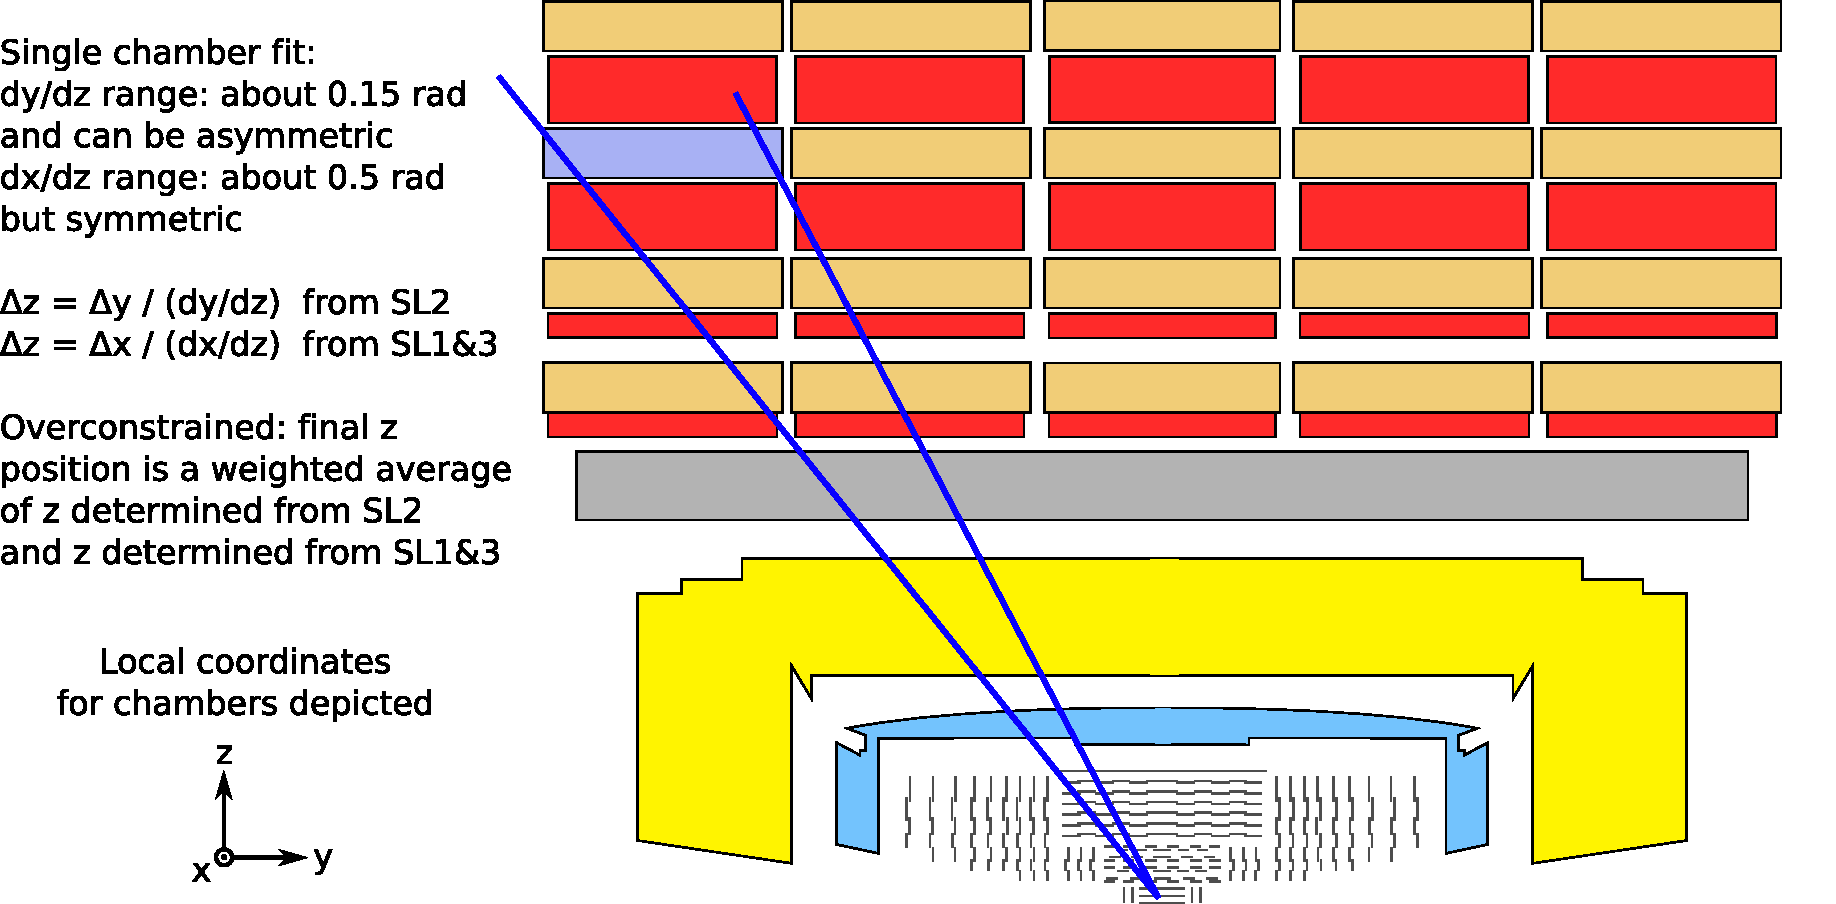
\includegraphics[width=\linewidth]{zfits_normal.pdf}
\end{frame}

\begin{frame}
\frametitle{Alternative under consideration}
\begin{itemize}
\item First fit $\delta_z$ for all wheels in same sector and station \mbox{(SemiSuperSector)\hspace{-1 cm}}
\item Then align one chamber at a time, keeping $\delta_z$ (and $\delta_{\phi_x}$) fixed
\item Huge range in $\frac{dy}{dz}$ would yield more precise result
\item Assumes hardware alignment has made all five $\delta_z$ values consistent!
\end{itemize}

\vfill
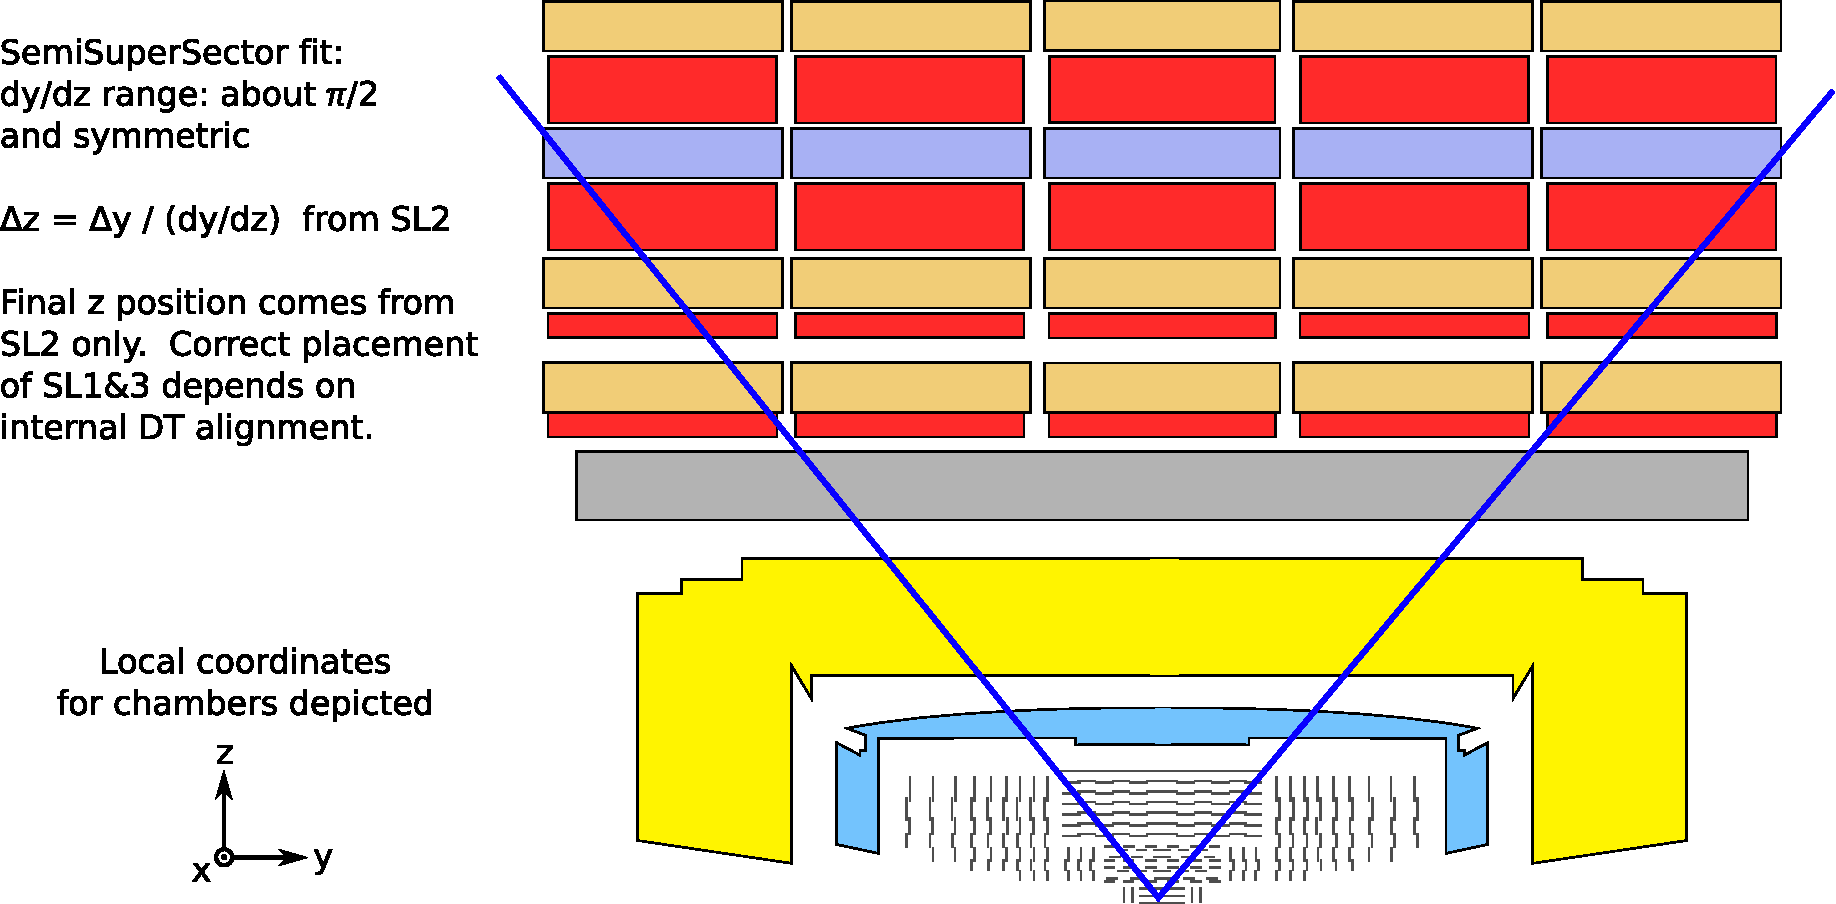
\includegraphics[width=\linewidth]{zfits_alternative.pdf}
\end{frame}

\begin{frame}
\frametitle{Fit method}
\begin{itemize}
\item Start with $\Delta y$ residual vs.~$\frac{dy}{dz}$ entrance
  angle plots with only hardware alignment and global adjustment
  applied: at most 5 plots (some plots are not available; they're taken from other diagnostics)
\item Fit them all with a single function: linear with the same slope
  (same~$\delta_z$), but potentially different intercepts (different~$\delta_y$)
\item Careful with signs! \mbox{($y$ and $\frac{dy}{dz}$ flip for wheels $+$1, $+$2 and some wheel~0)\hspace{-2 cm}}
\end{itemize}

\vfill \centering
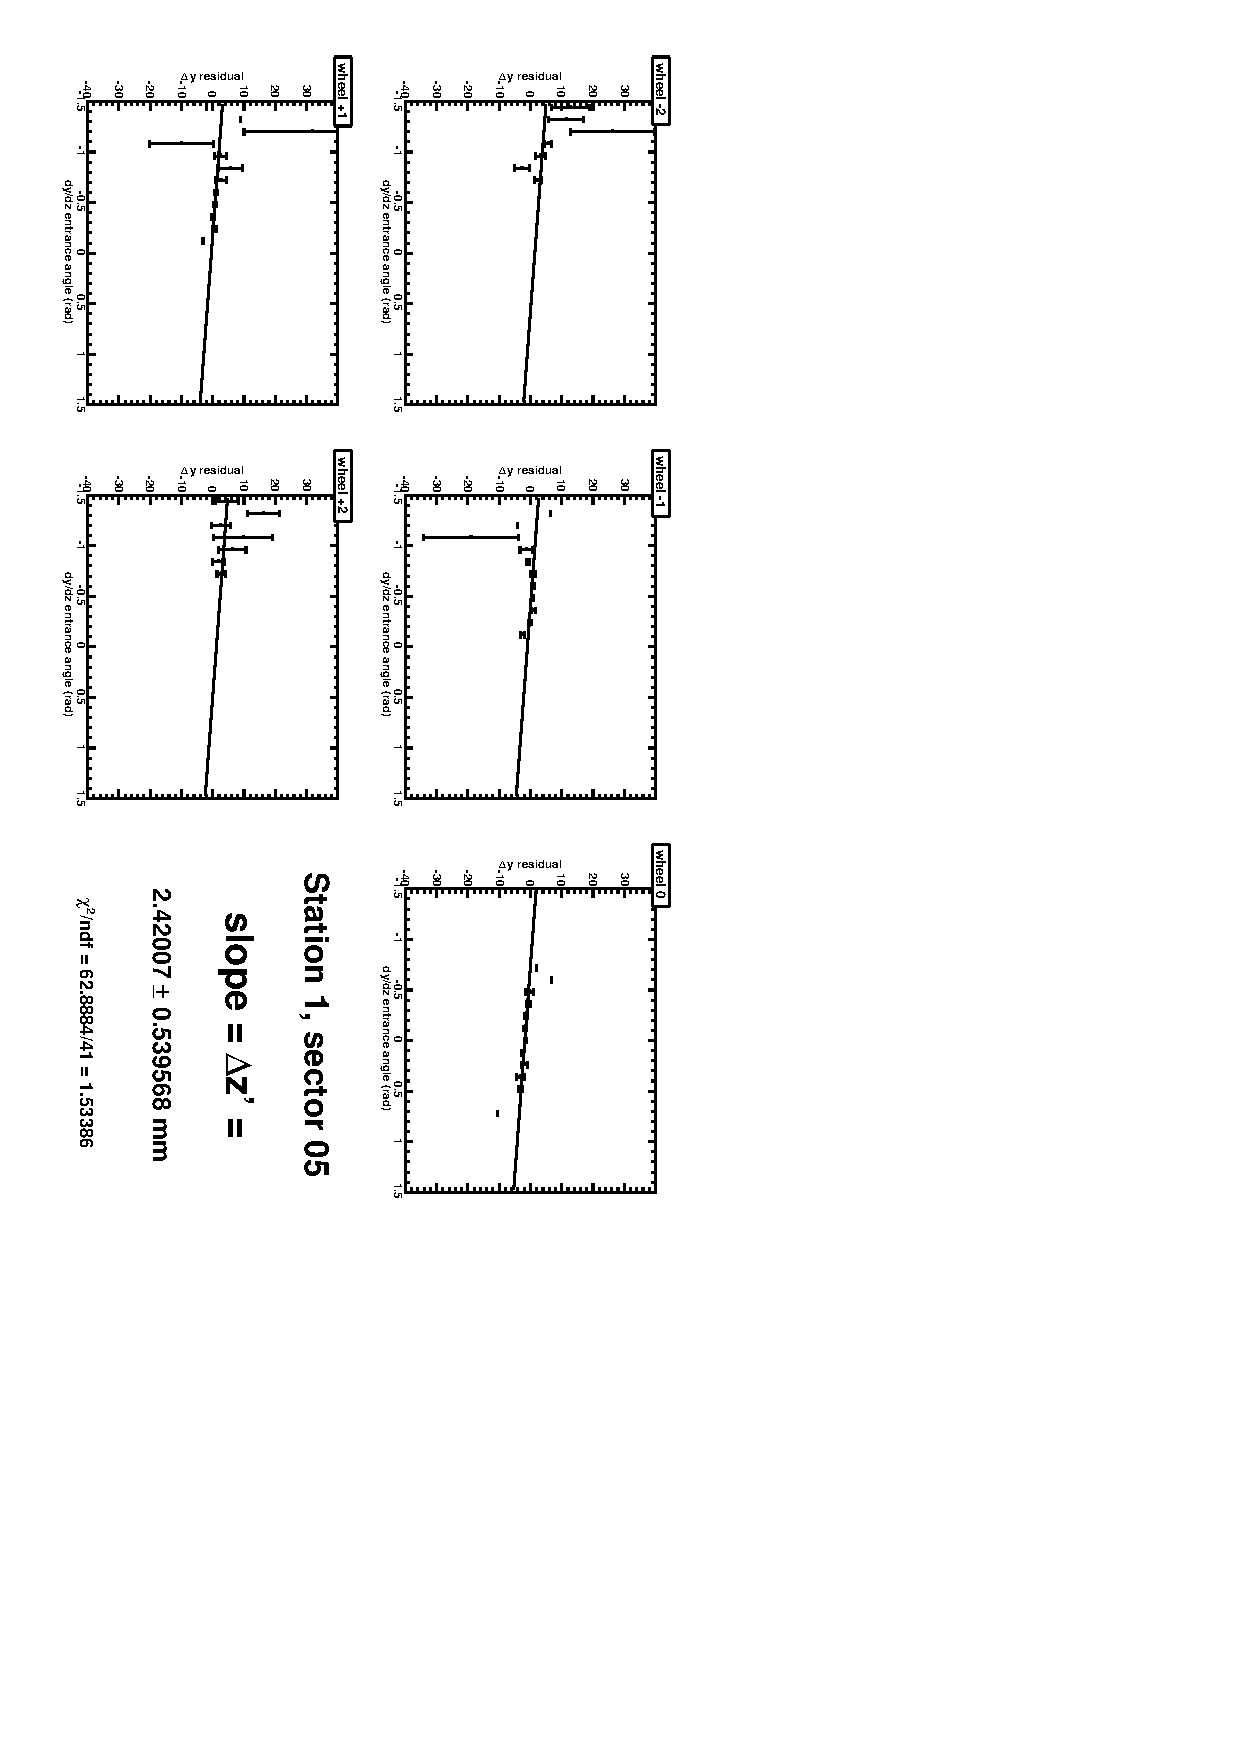
\includegraphics[height=0.9\linewidth, angle=90]{zfits/zfit_1_05.pdf}
\end{frame}

\begin{frame}
\frametitle{Summary of fit results}
\label{summary}

\vspace{-0.75 cm}
\begin{columns}
\column{0.7\linewidth}
\vspace{0.5 cm}
\begin{itemize}
\item $\chi^2$ are reasonable (all wheels in each sector are roughly consistent)
\item Semi-regular pattern inside all of the SuperSectors (dashed lines)
\item Individual fits on the pages that follow
\end{itemize}
\column{0.3\linewidth}
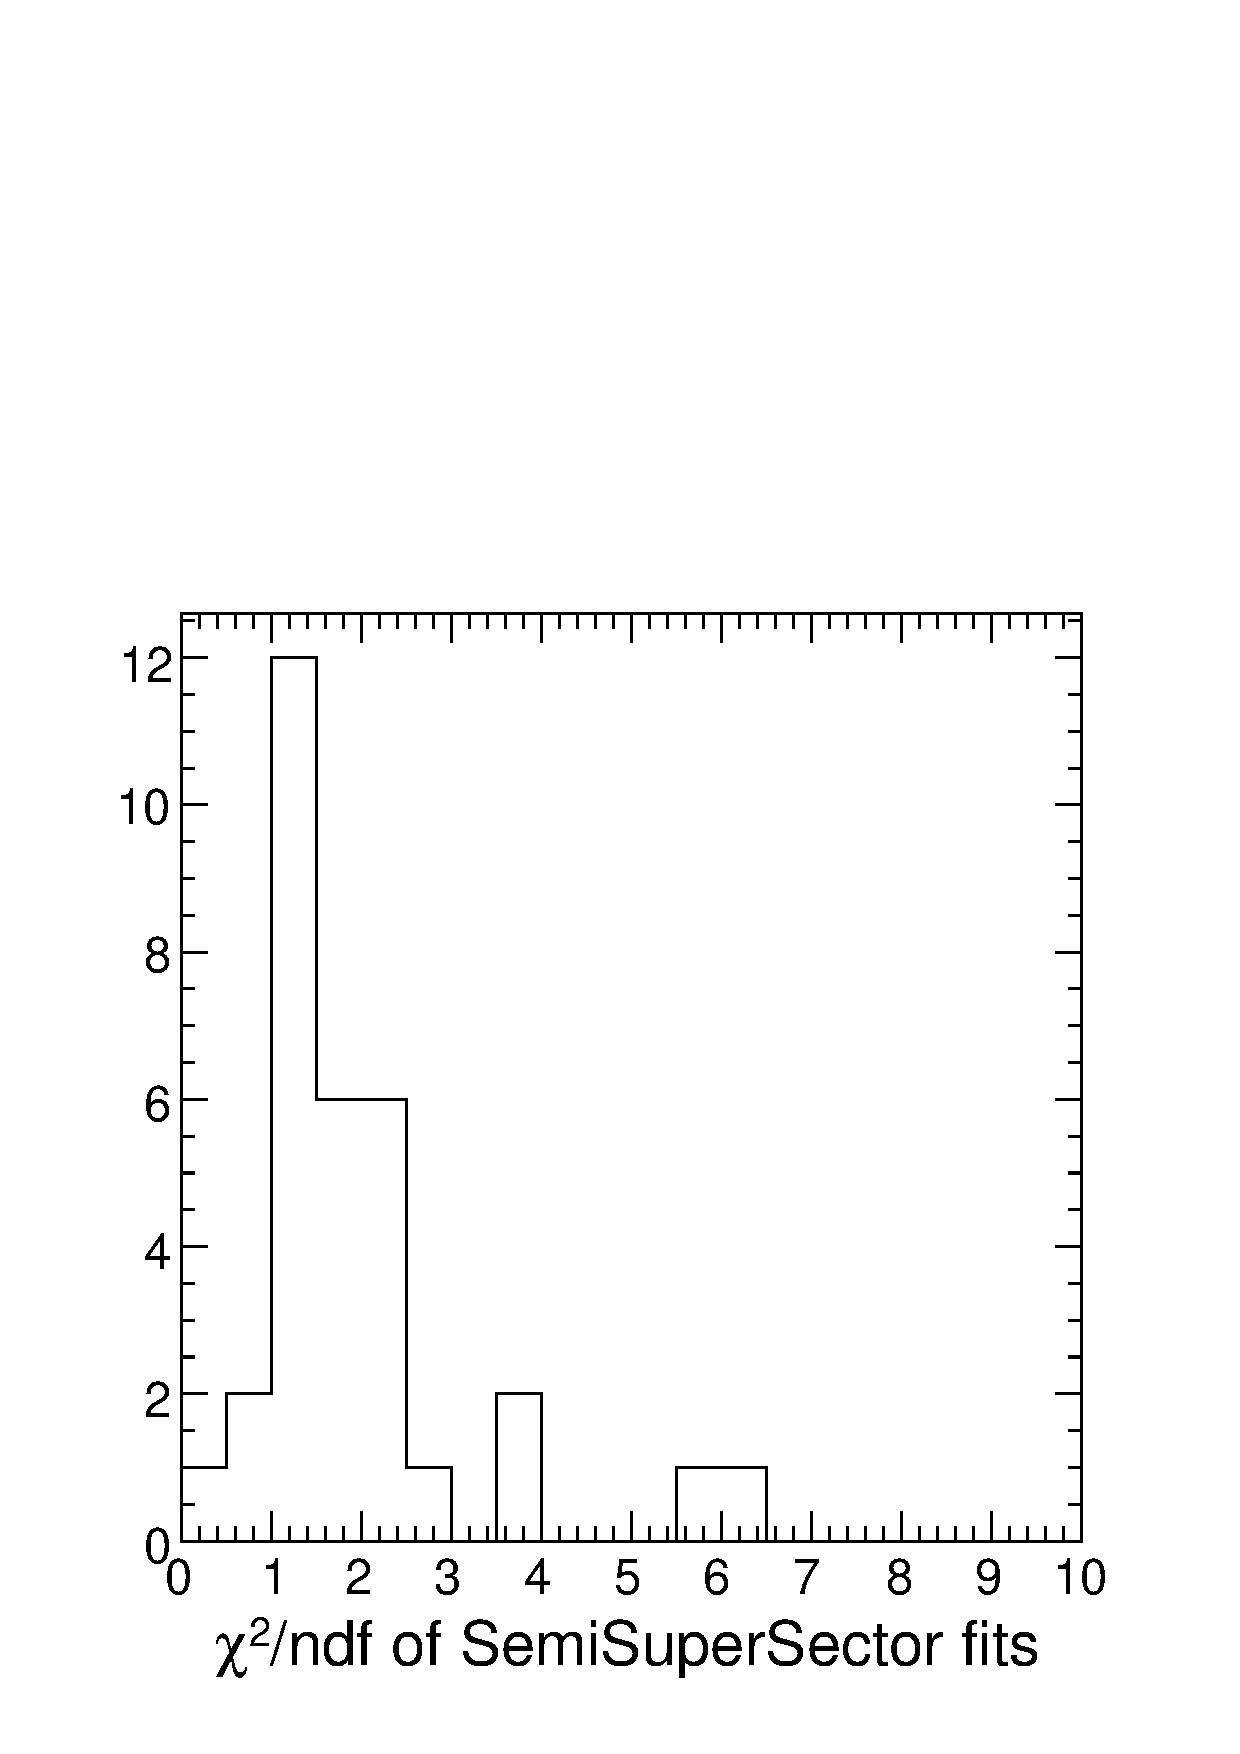
\includegraphics[width=\linewidth]{zfits_chi2.pdf}
\end{columns}

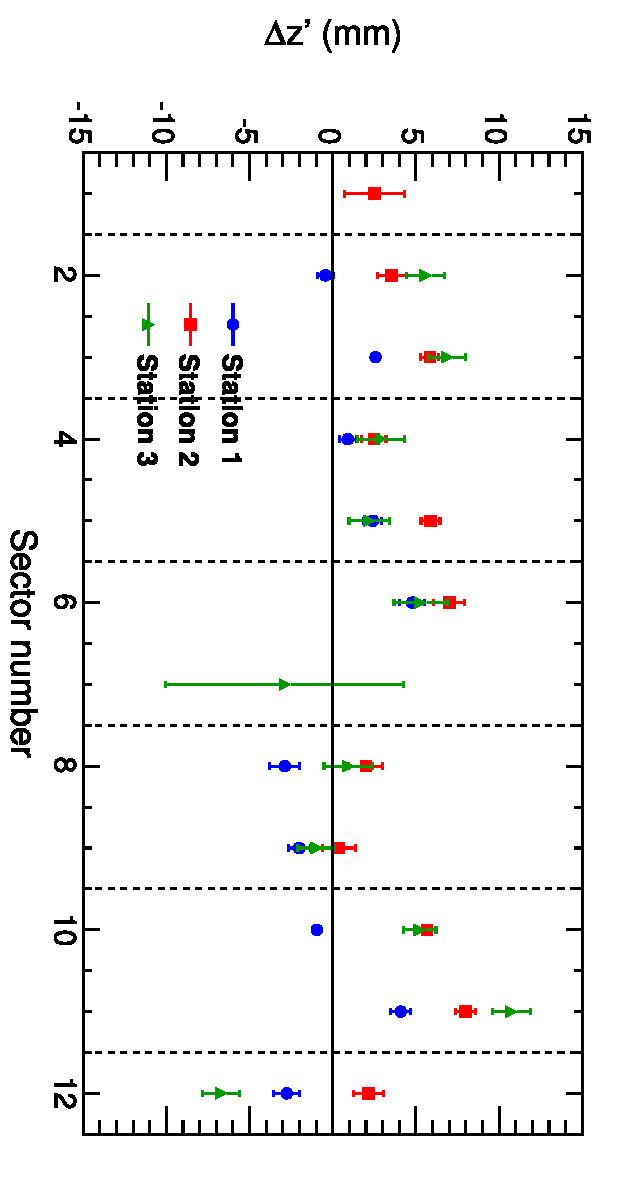
\includegraphics[height=\linewidth, angle=90]{zfits_stations.pdf}
\end{frame}

\begin{frame}
\frametitle{Station 1, sector 2}
\begin{columns}
\column{0.7\linewidth}
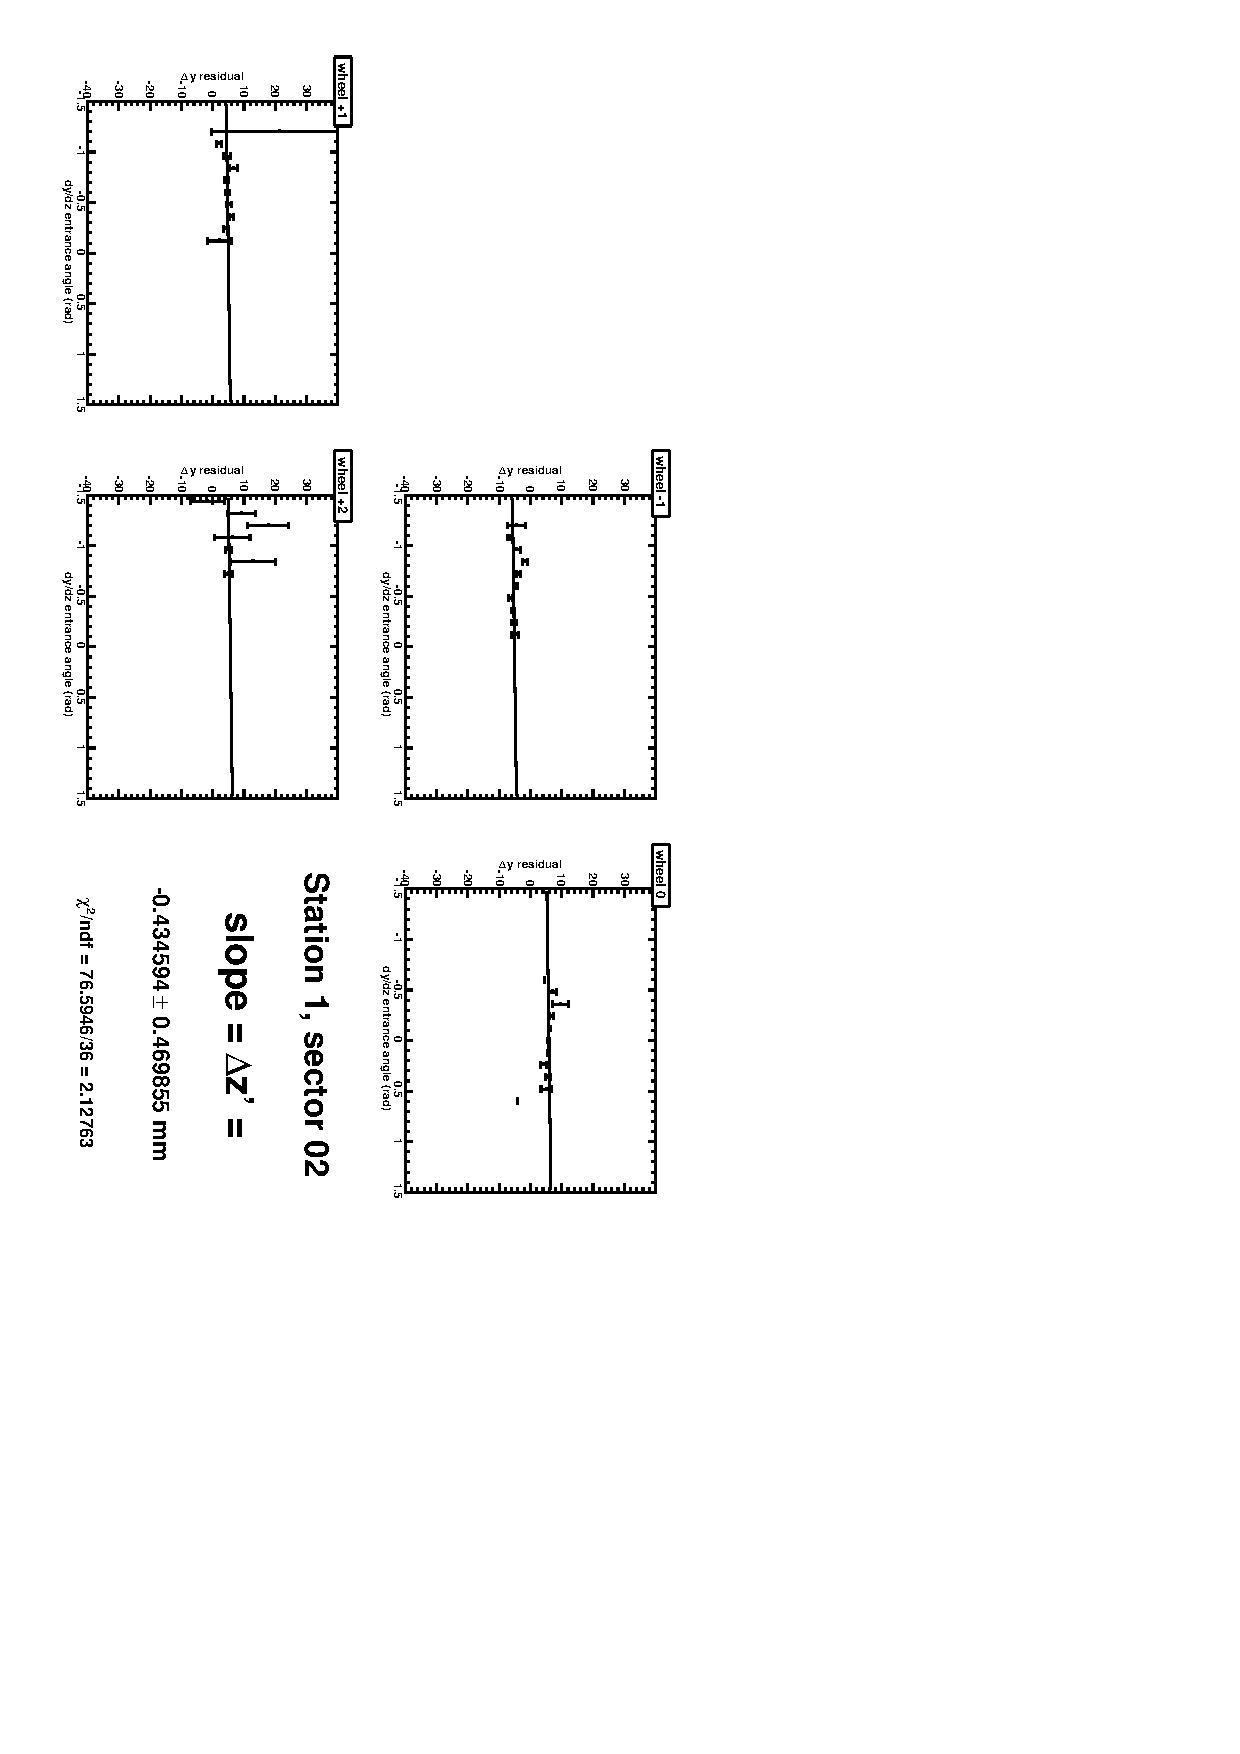
\includegraphics[height=\linewidth, angle=90]{zfits/zfit_1_02.pdf}

\vfill
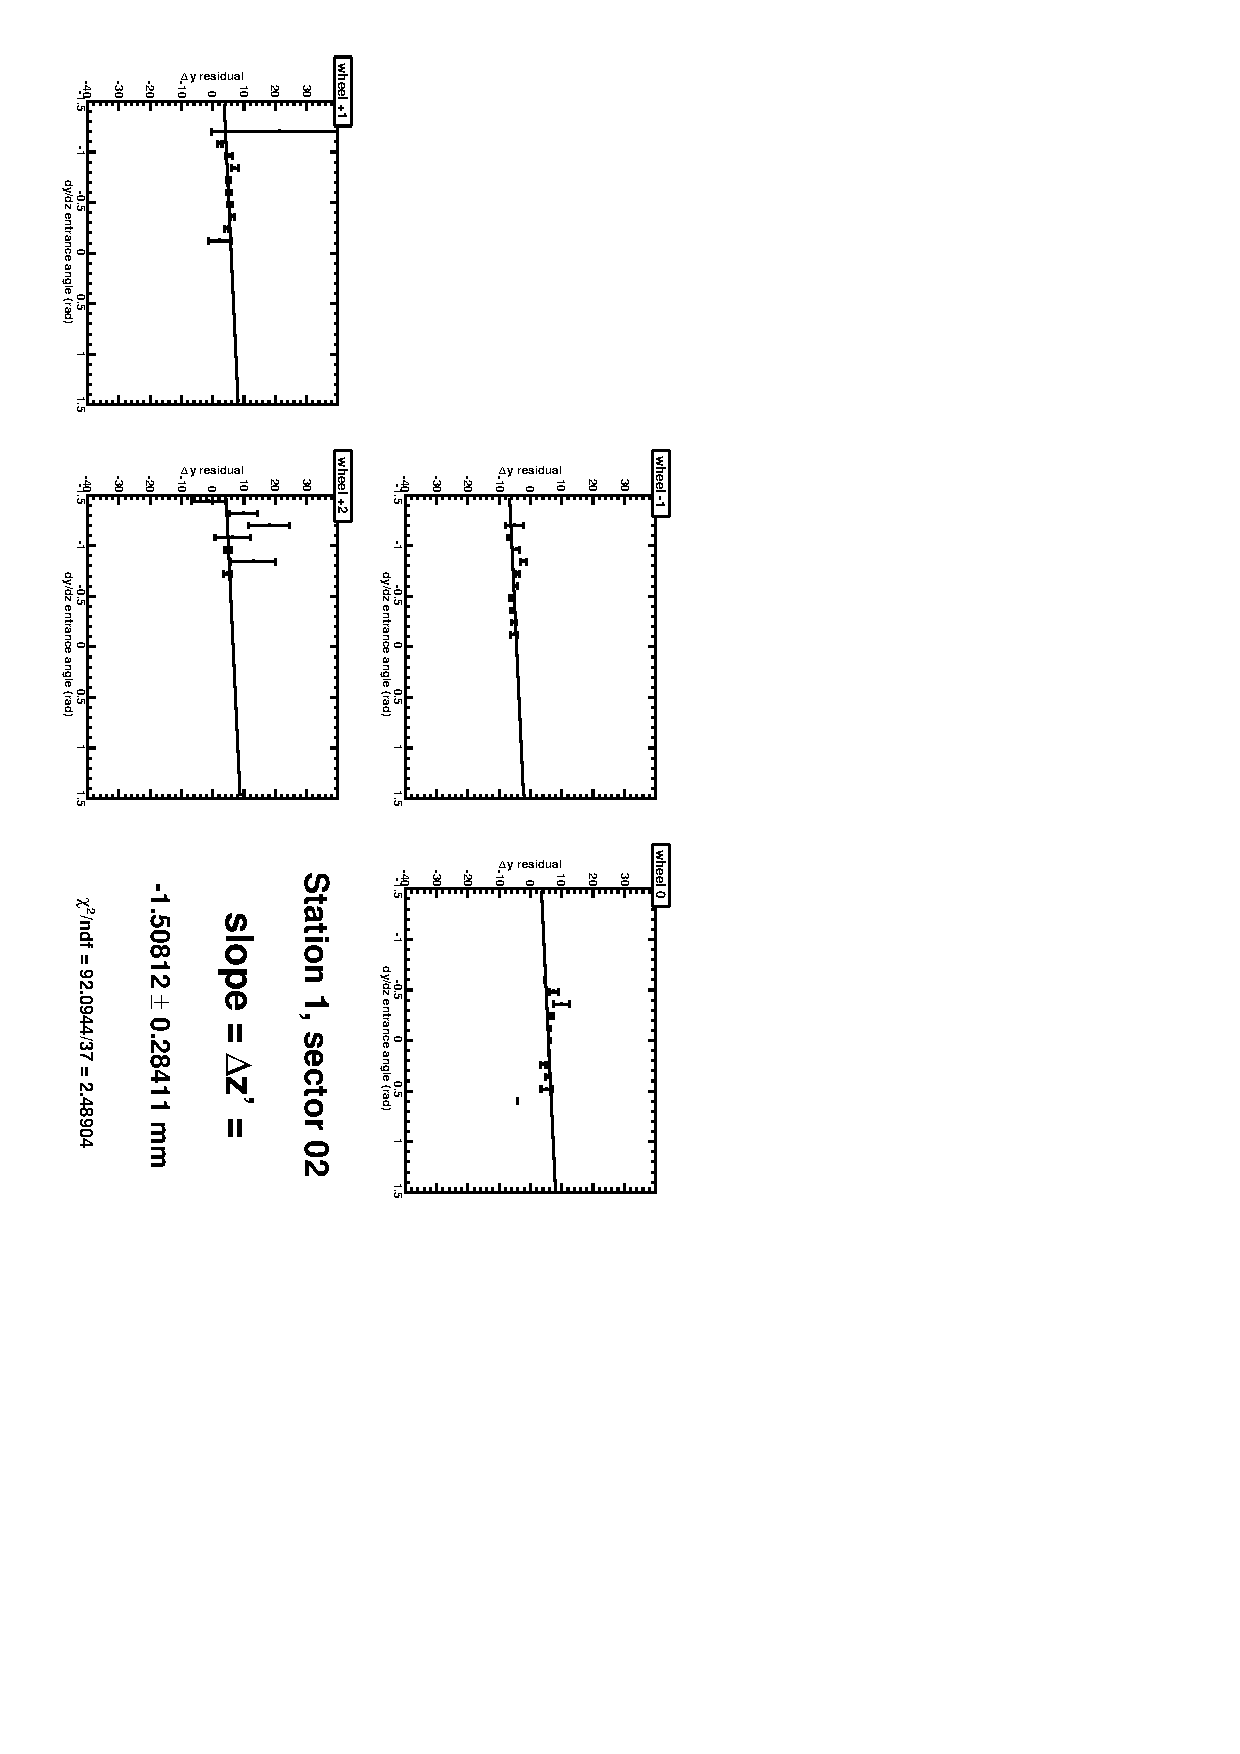
\includegraphics[height=\linewidth, angle=90]{zfits_after/zfit_1_02.pdf}
\column{0.3\linewidth}
\begin{itemize}
\item Top: before \\ Bottom: after
\item Five panels are wheels in the same SemiSuperSector (some are missing)
\item Fit requires all to have the same slope ($\delta_z$), but allows different offsets ($\delta_y$)
\item This first one is a weak fit: keep going \mbox{(to page~\pageref{after})\hspace{-1 cm}}
\end{itemize}
\end{columns}
\end{frame}

\begin{frame}
\frametitle{Station 1, sector 3}
\begin{columns}
\column{0.7\linewidth}
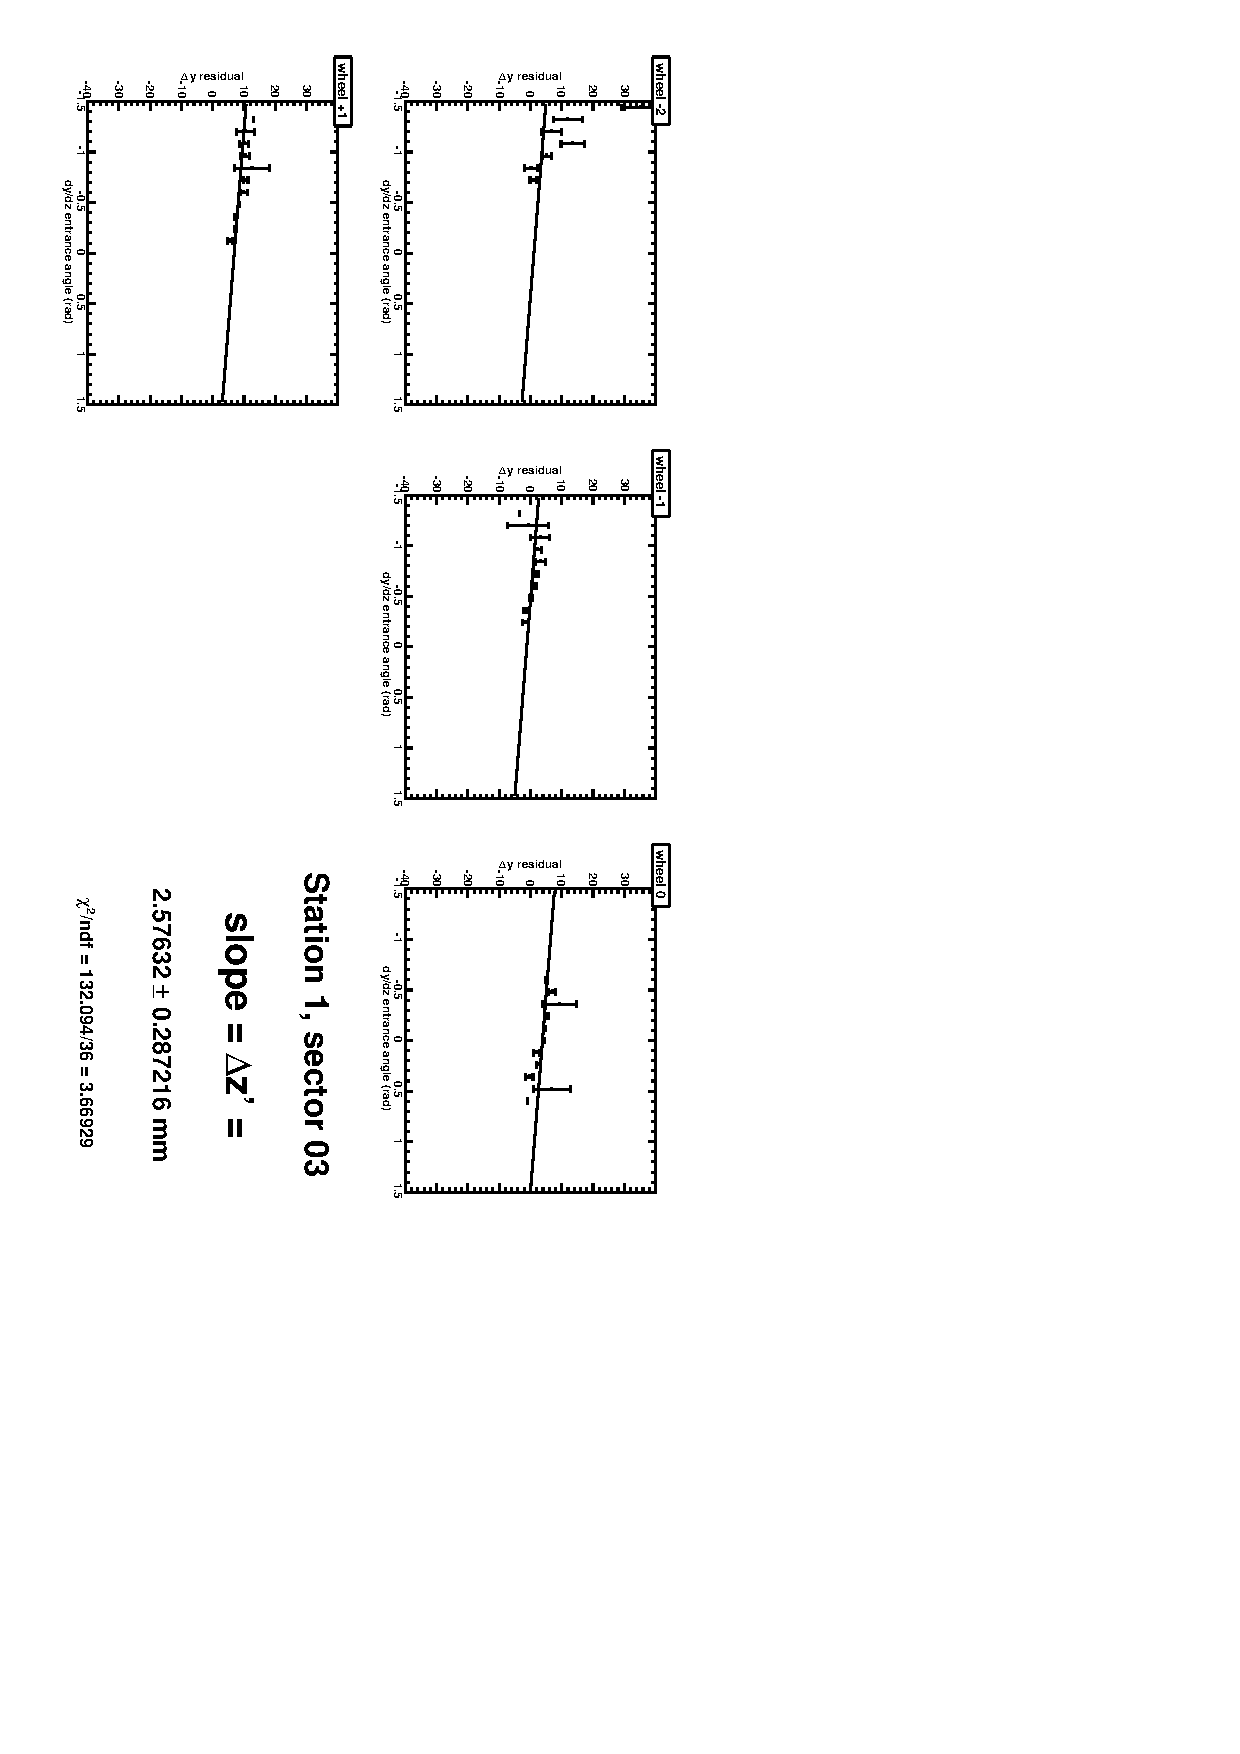
\includegraphics[height=\linewidth, angle=90]{zfits/zfit_1_03.pdf}

\vfill
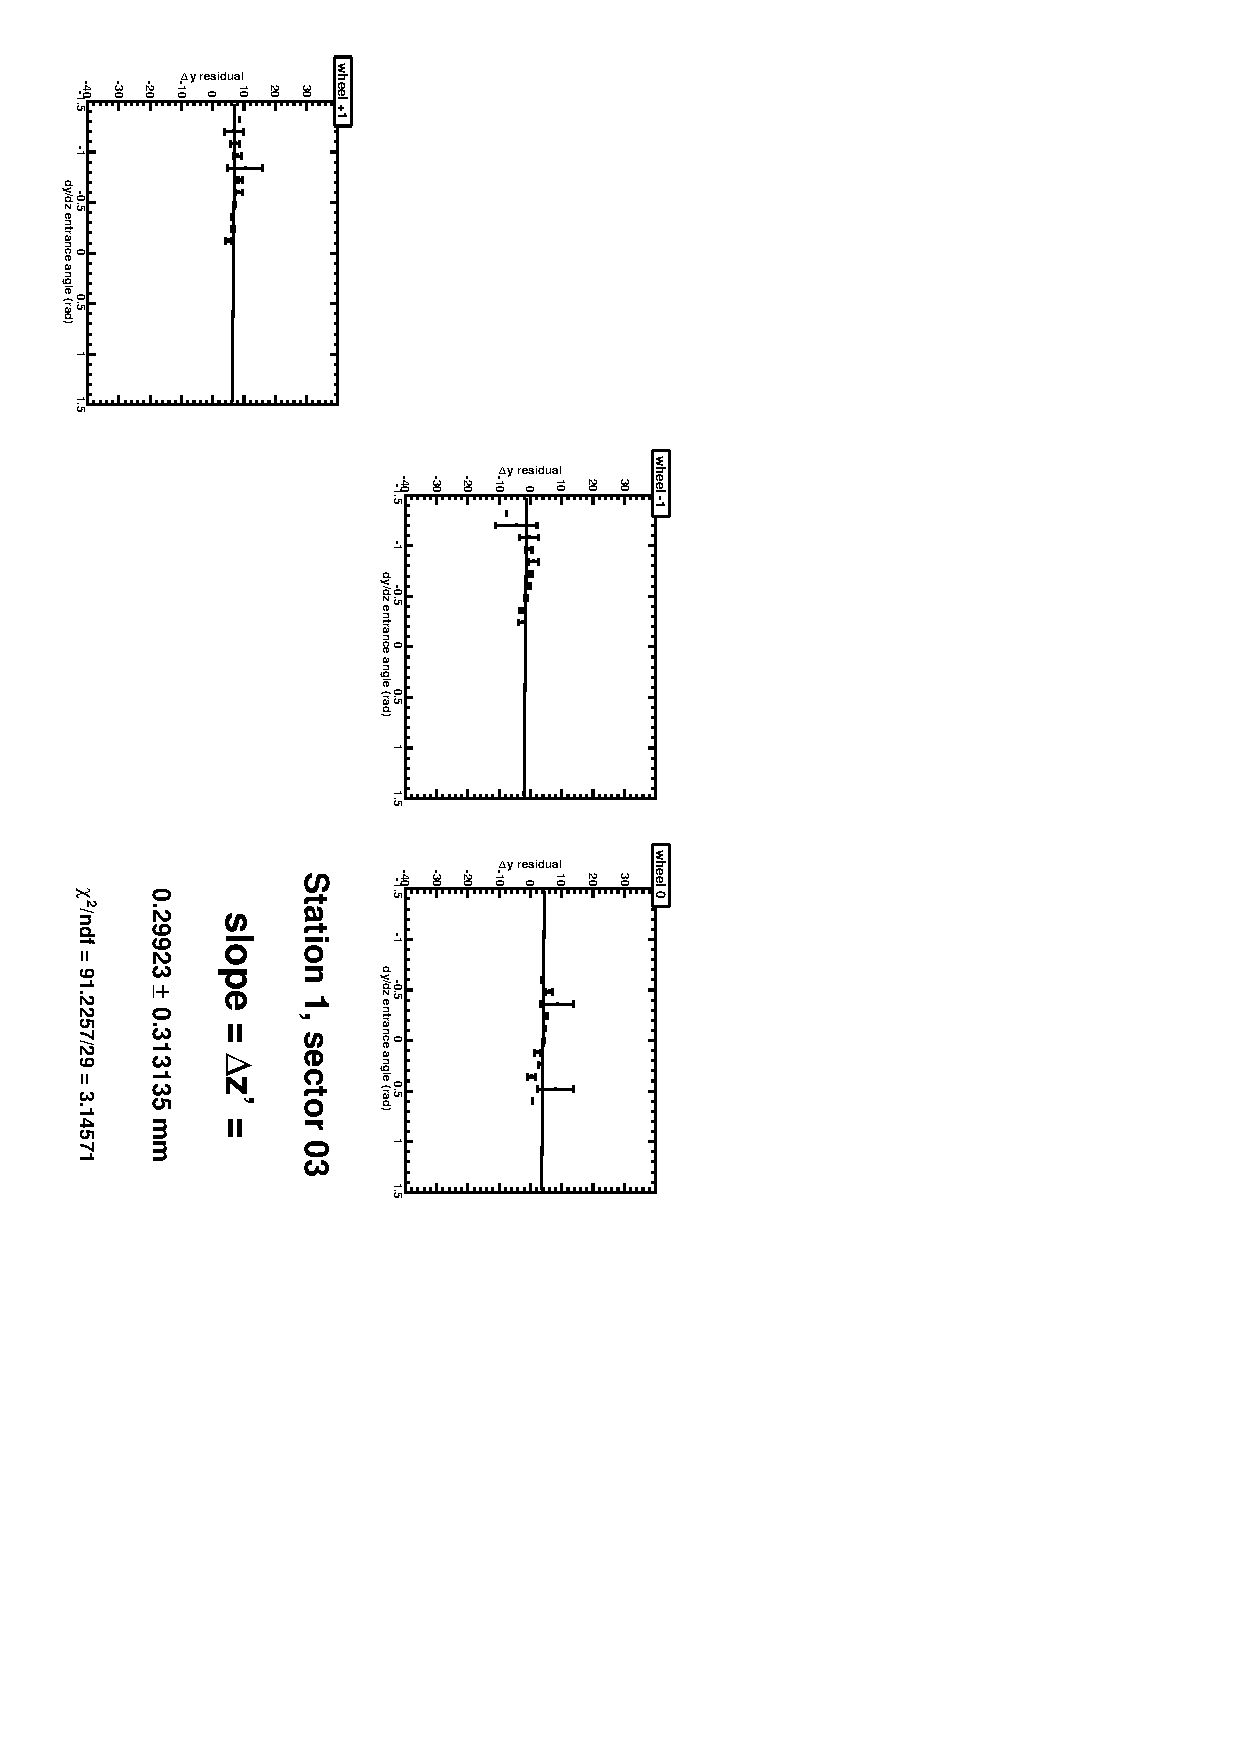
\includegraphics[height=\linewidth, angle=90]{zfits_after/zfit_1_03.pdf}
\column{0.3\linewidth}
\begin{itemize}
\item Top: before \\ Bottom: after
\item Five panels are wheels in the same SemiSuperSector (some are missing)
\item Fit requires all to have the same slope ($\delta_z$), but allows different offsets ($\delta_y$)
\end{itemize}
\end{columns}
\end{frame}

\begin{frame}
\frametitle{Station 1, sector 4}
\begin{columns}
\column{0.7\linewidth}
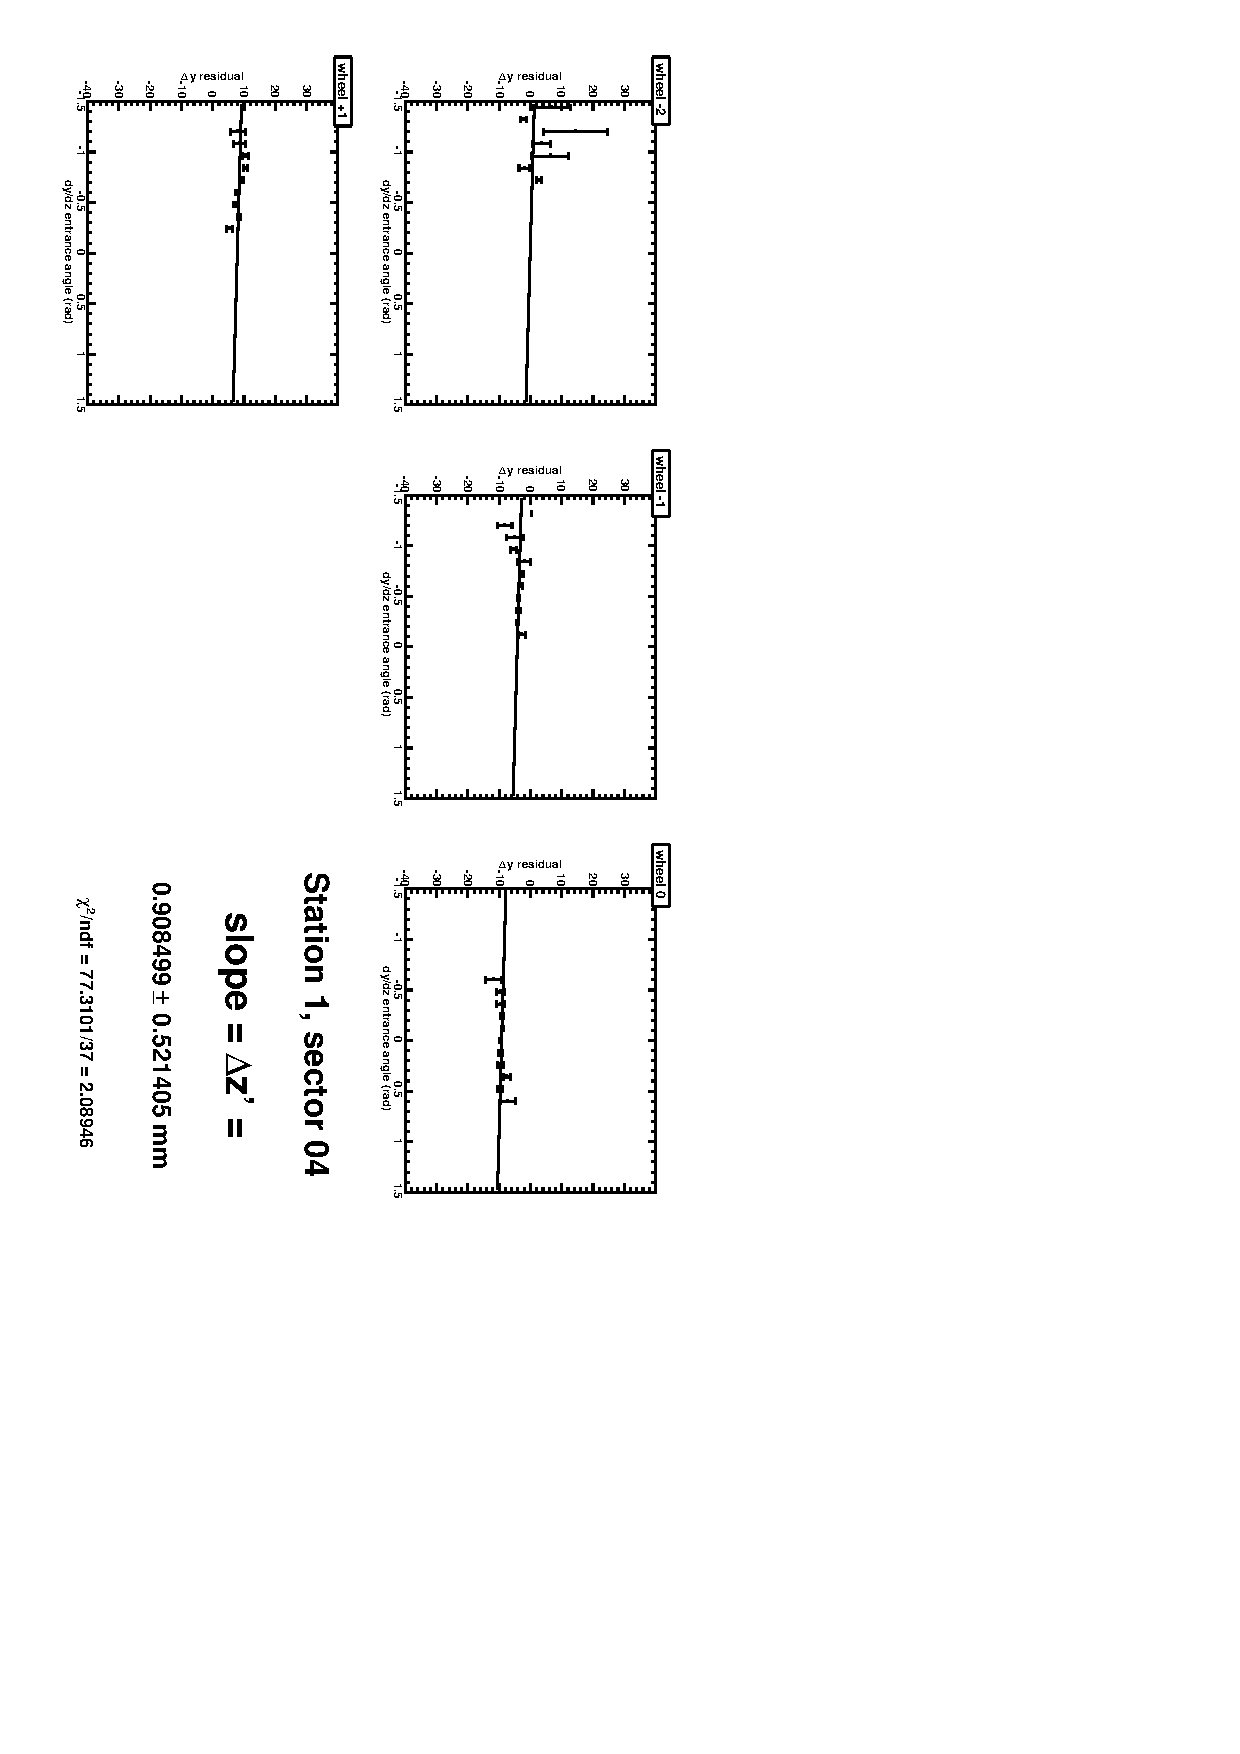
\includegraphics[height=\linewidth, angle=90]{zfits/zfit_1_04.pdf}

\vfill
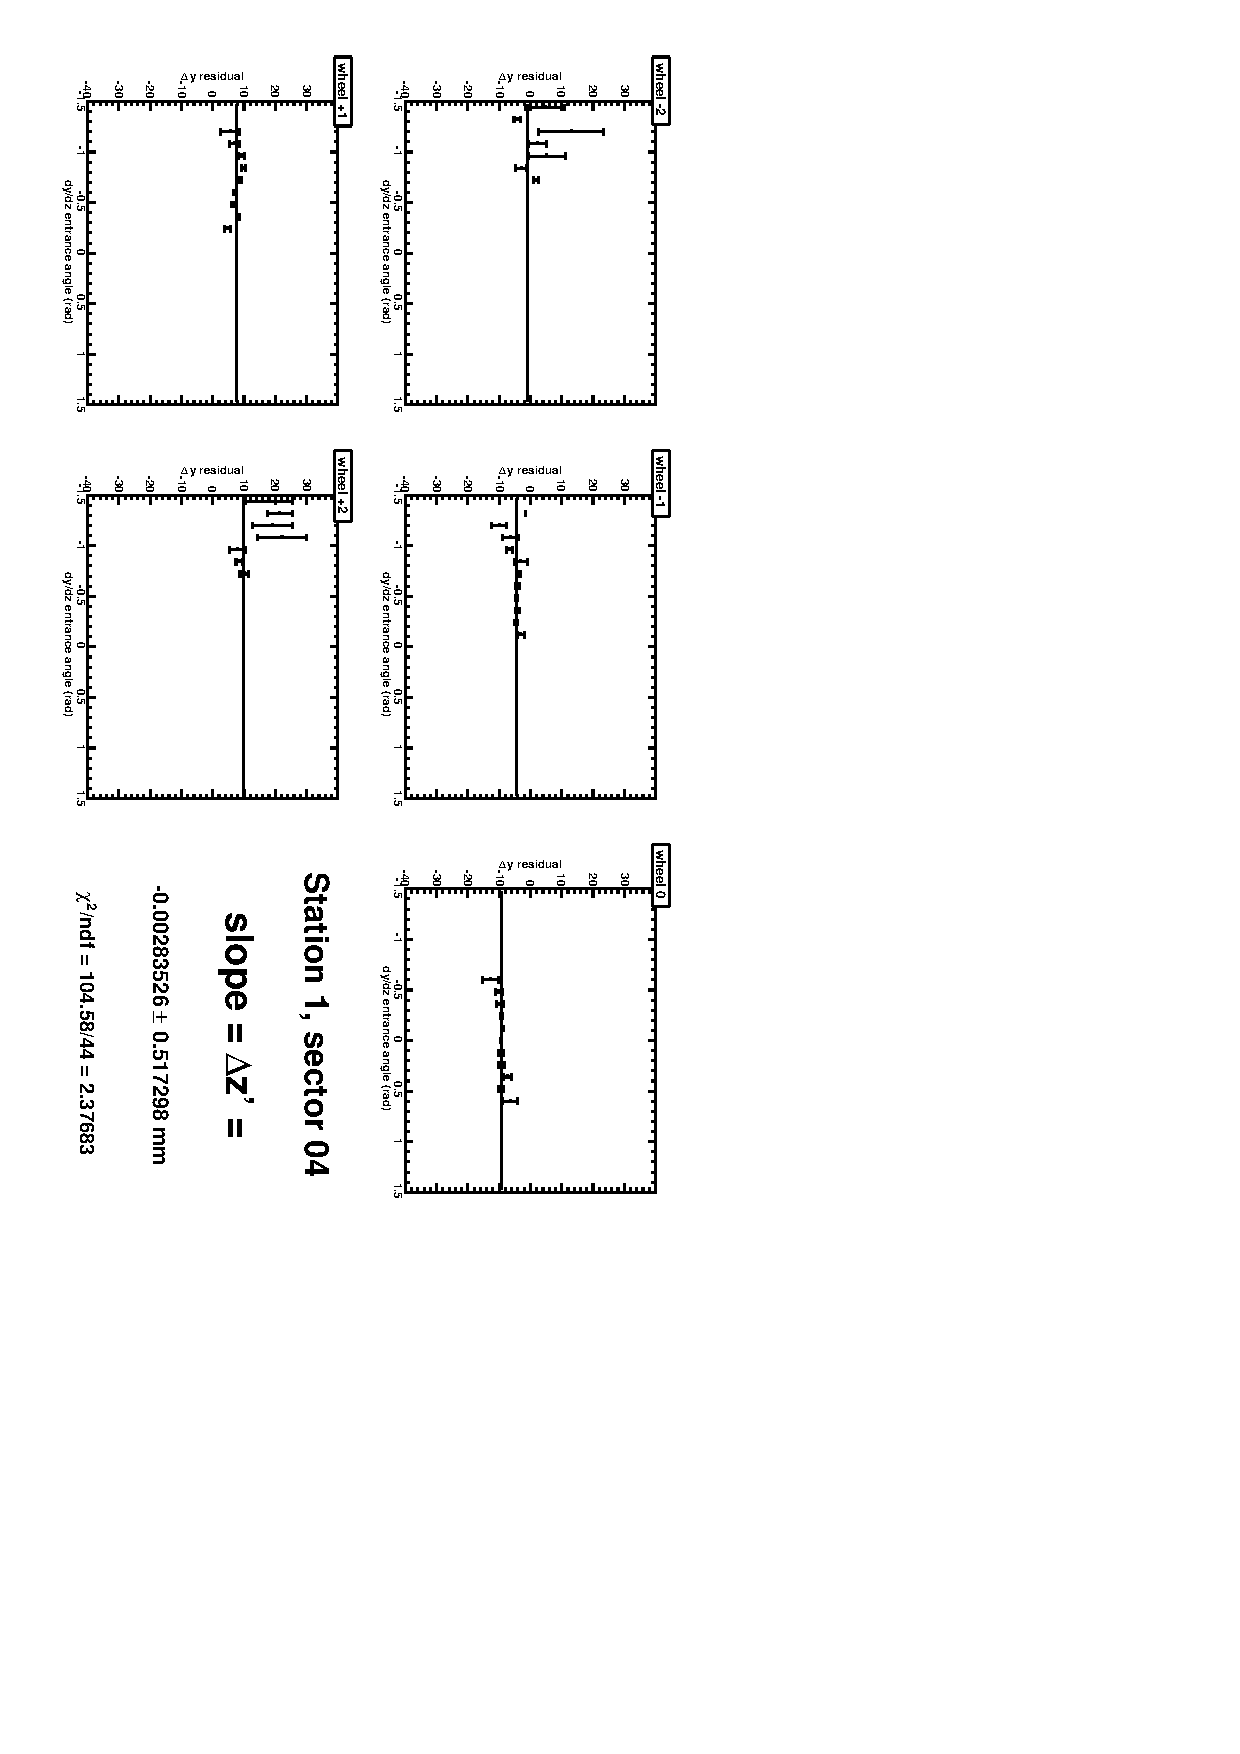
\includegraphics[height=\linewidth, angle=90]{zfits_after/zfit_1_04.pdf}
\column{0.3\linewidth}
\begin{itemize}
\item Top: before \\ Bottom: after
\item Five panels are wheels in the same SemiSuperSector (some are missing)
\item Fit requires all to have the same slope ($\delta_z$), but allows different offsets ($\delta_y$)
\end{itemize}
\end{columns}
\end{frame}

\begin{frame}
\frametitle{Station 1, sector 5}
\begin{columns}
\column{0.7\linewidth}
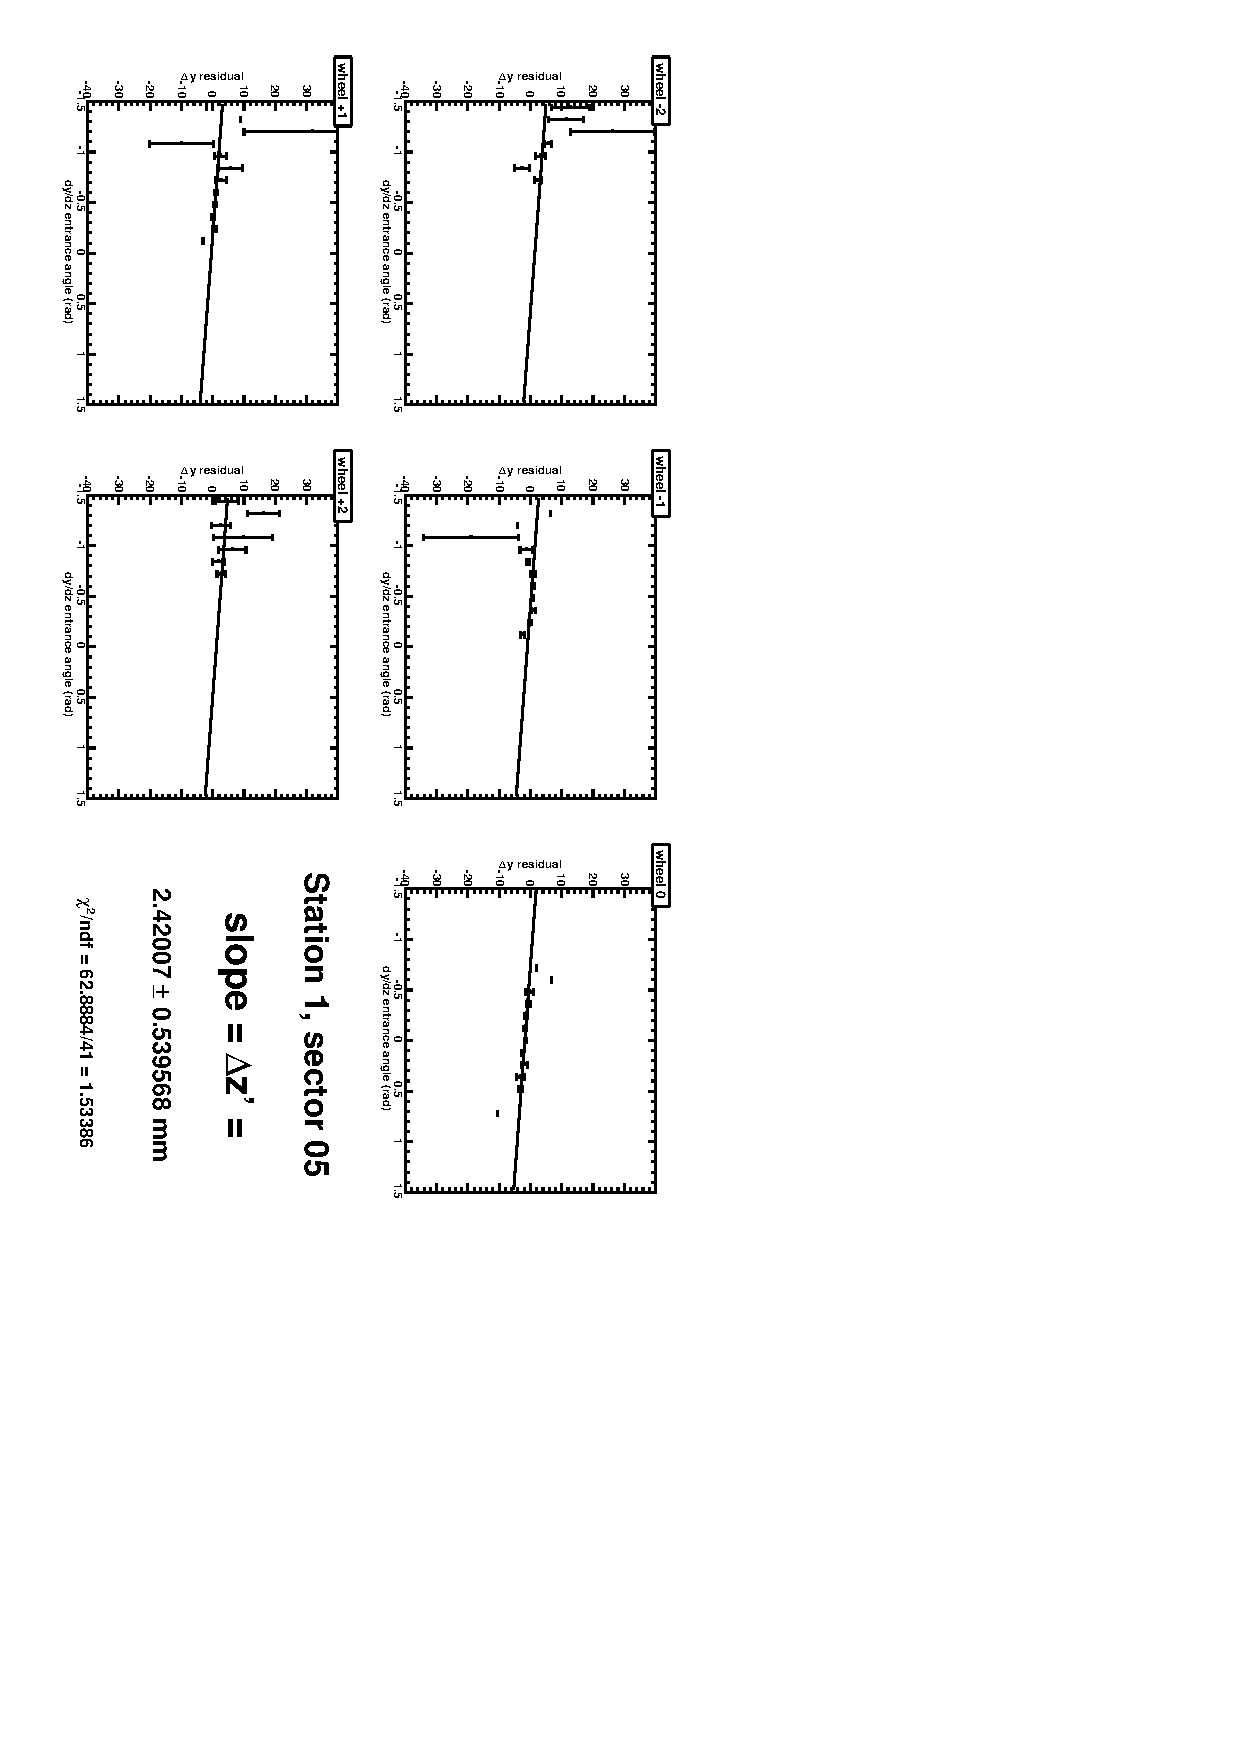
\includegraphics[height=\linewidth, angle=90]{zfits/zfit_1_05.pdf}

\vfill
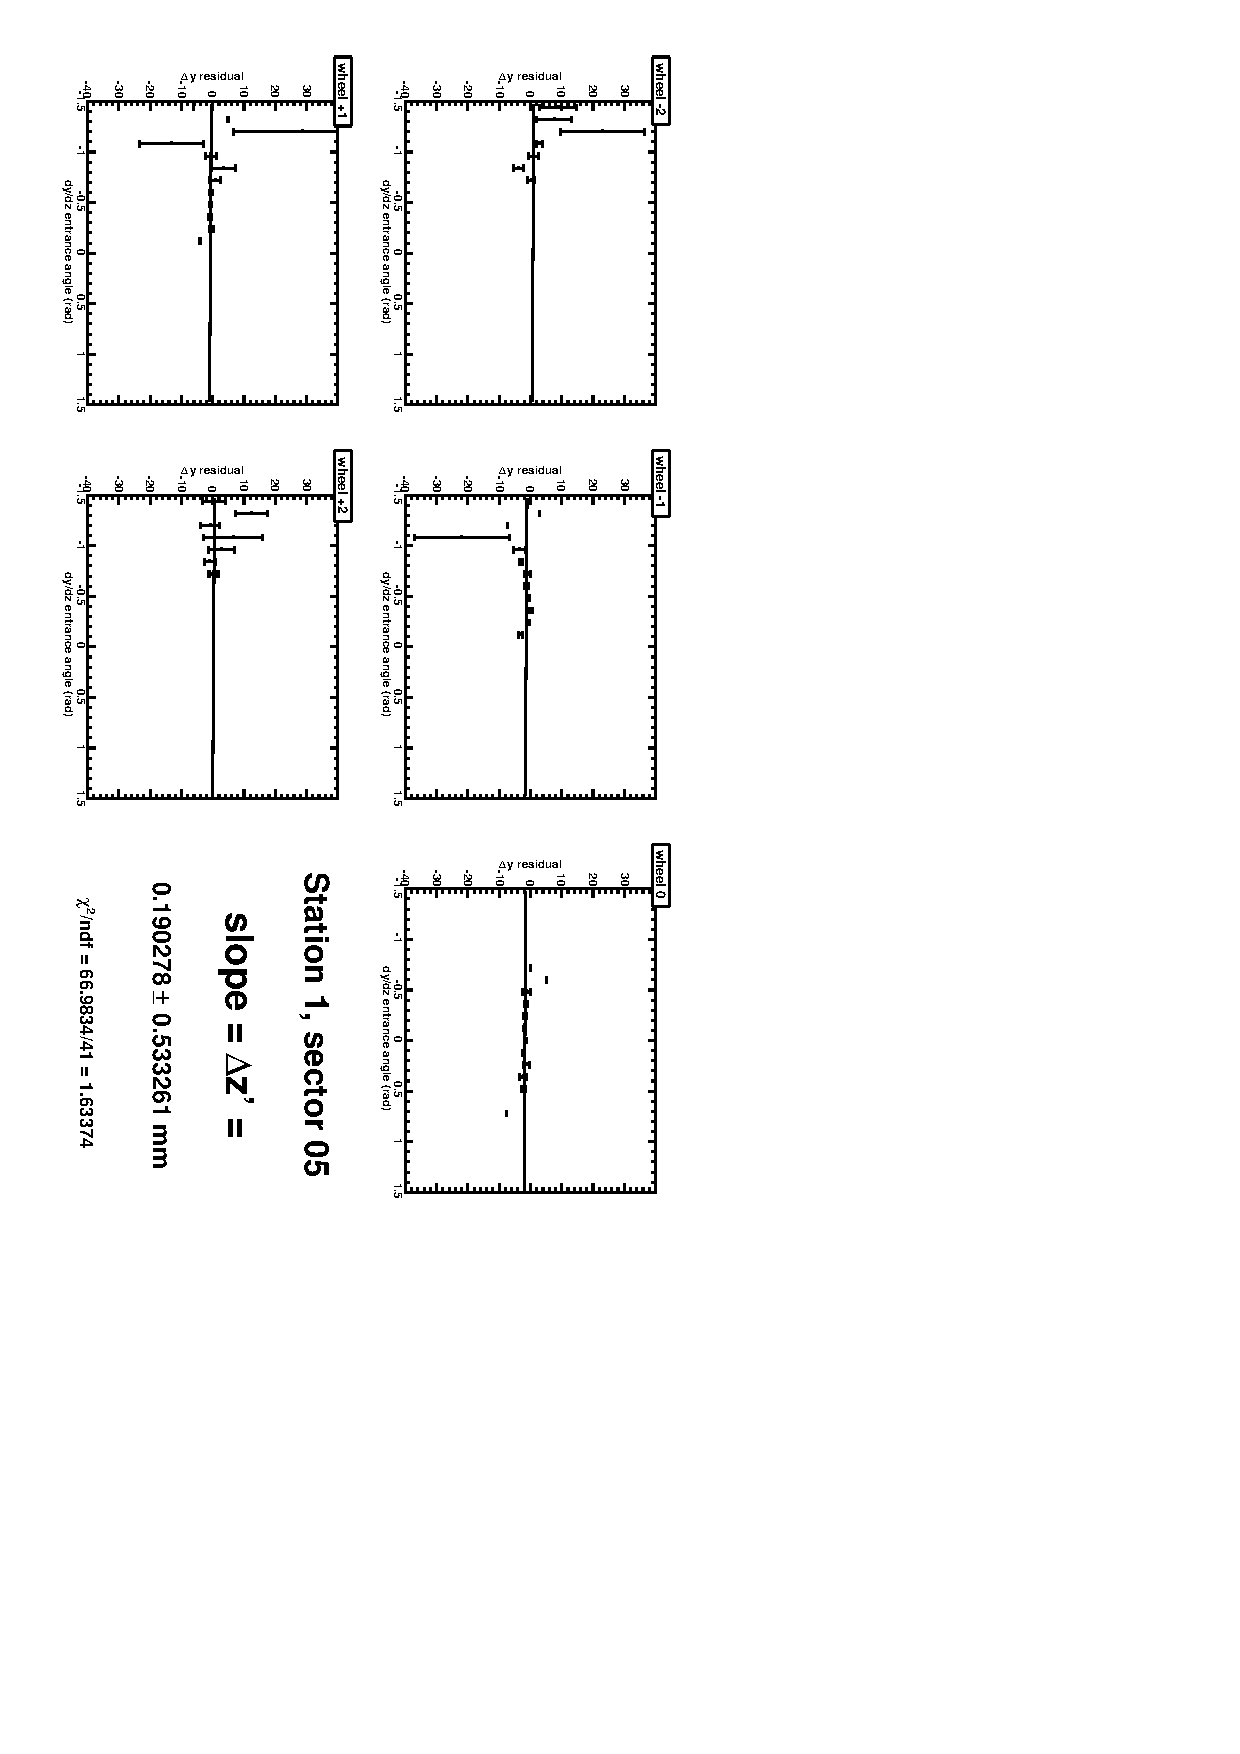
\includegraphics[height=\linewidth, angle=90]{zfits_after/zfit_1_05.pdf}
\column{0.3\linewidth}
\begin{itemize}
\item Top: before \\ Bottom: after
\item Five panels are wheels in the same SemiSuperSector (some are missing)
\item Fit requires all to have the same slope ($\delta_z$), but allows different offsets ($\delta_y$)
\end{itemize}
\end{columns}
\end{frame}

\begin{frame}
\frametitle{Station 1, sector 6}
\begin{columns}
\column{0.7\linewidth}
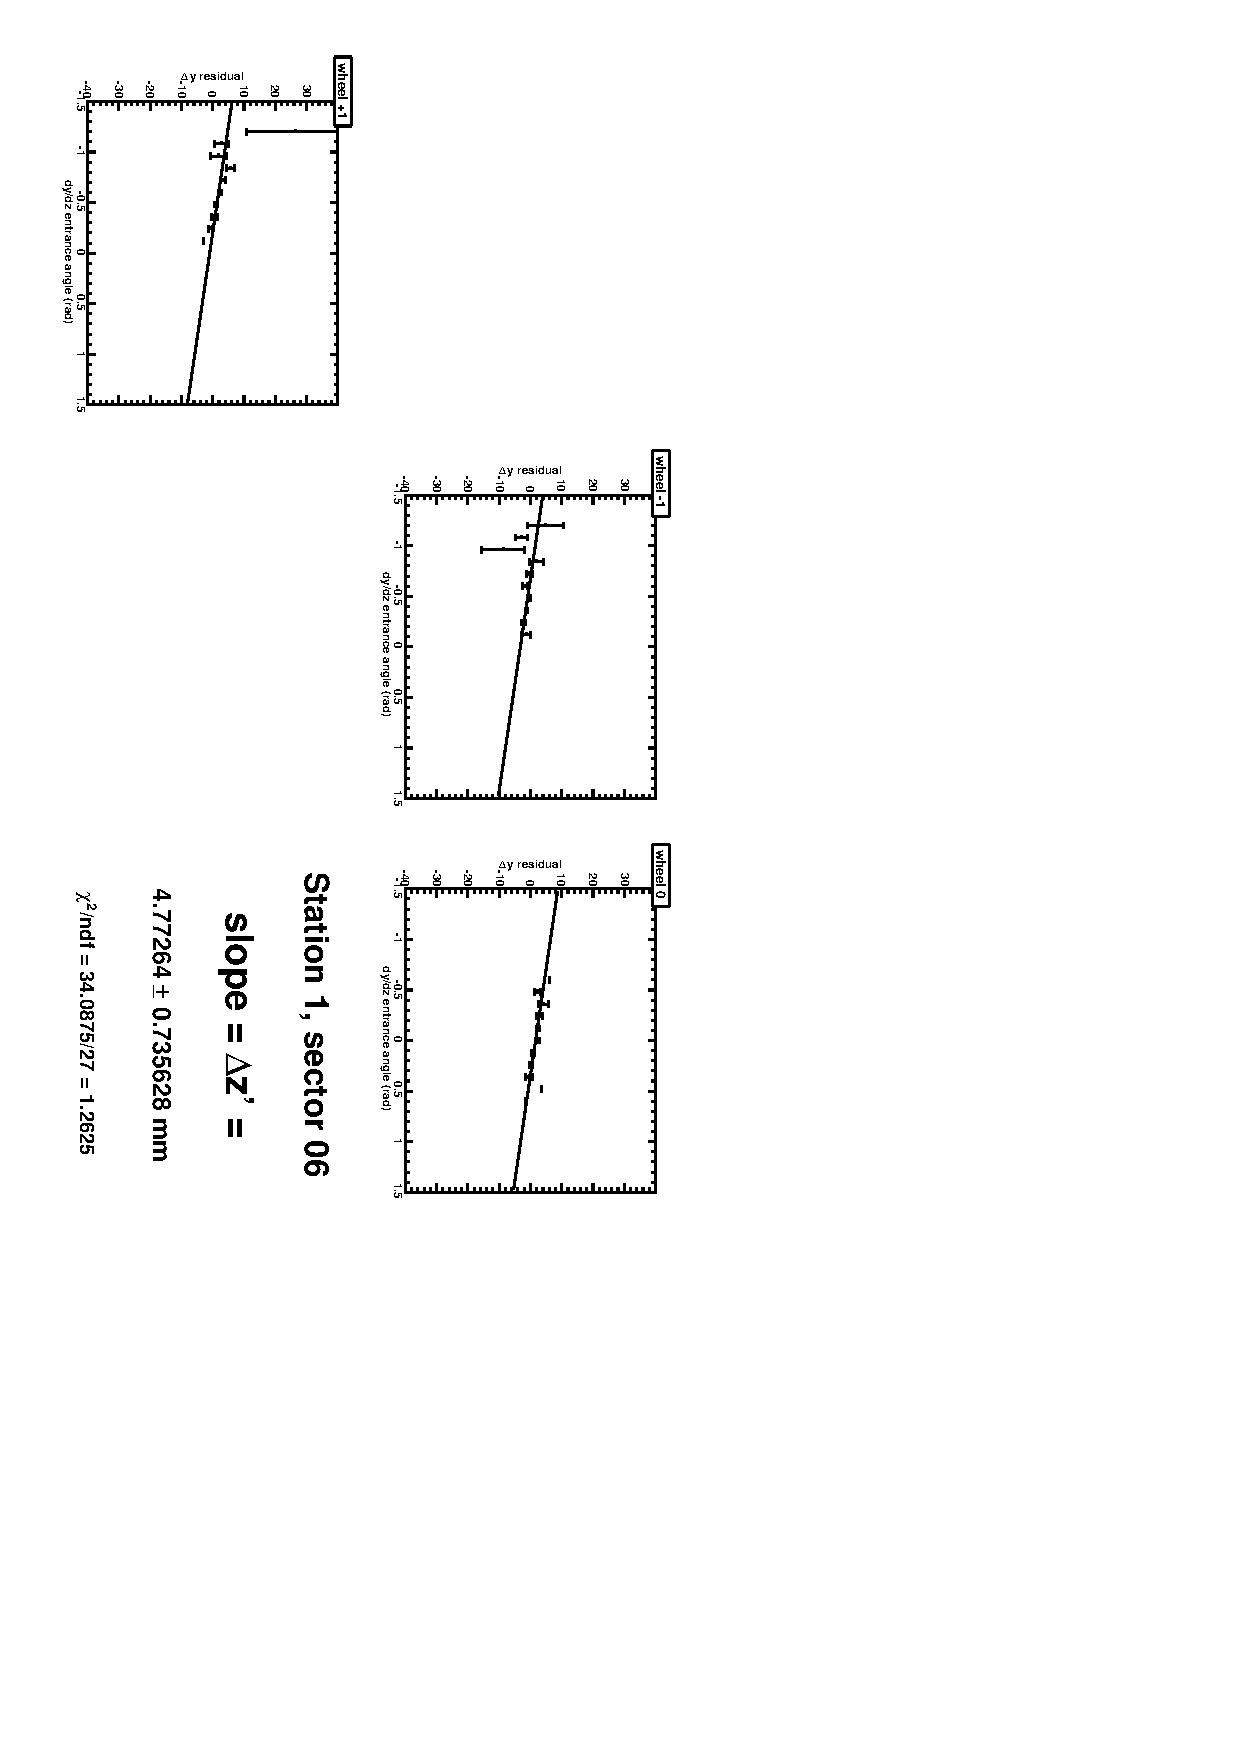
\includegraphics[height=\linewidth, angle=90]{zfits/zfit_1_06.pdf}

\vfill
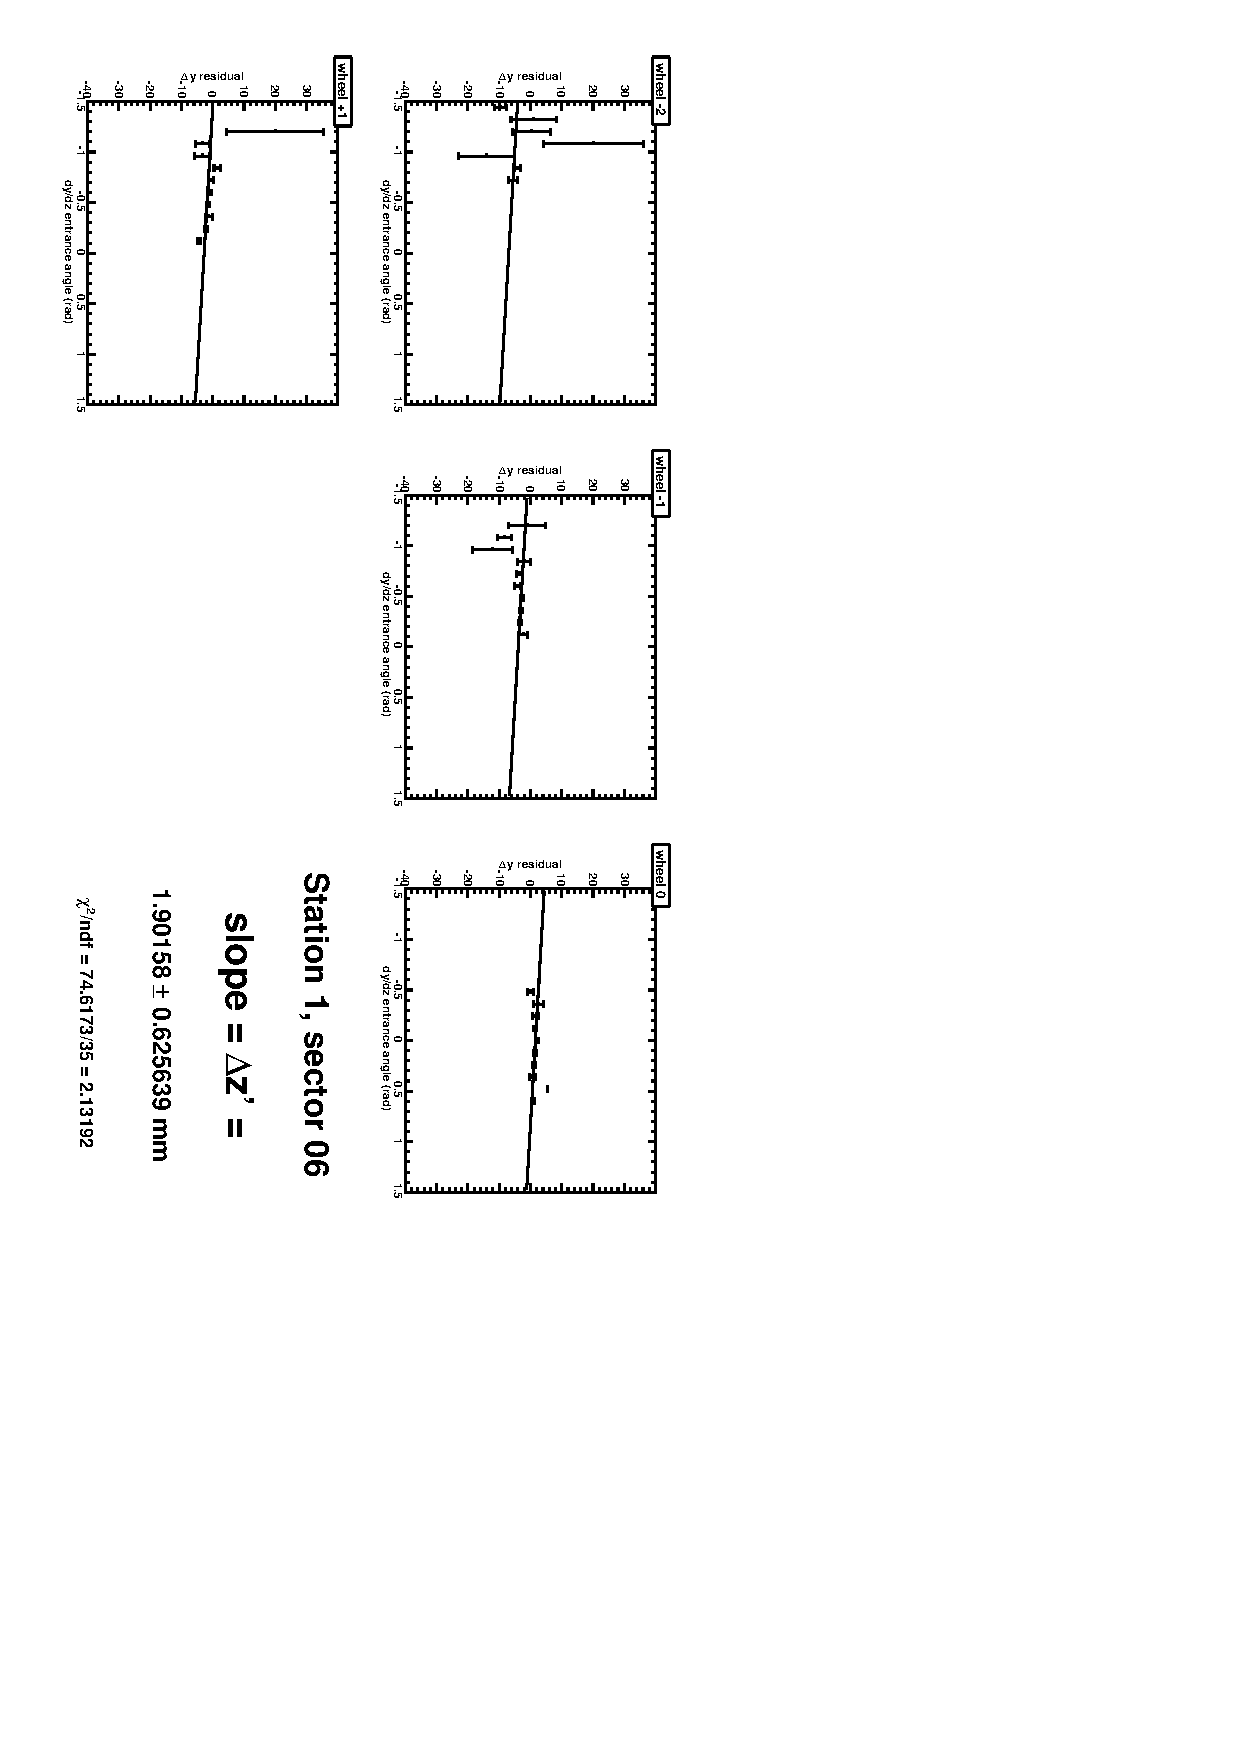
\includegraphics[height=\linewidth, angle=90]{zfits_after/zfit_1_06.pdf}
\column{0.3\linewidth}
\begin{itemize}
\item Top: before \\ Bottom: after
\item Five panels are wheels in the same SemiSuperSector (some are missing)
\item Fit requires all to have the same slope ($\delta_z$), but allows different offsets ($\delta_y$)
\item In general, fits are poor near the horizontals (sectors~1 and~7)
\end{itemize}
\end{columns}
\end{frame}

\begin{frame}
\frametitle{Station 1, sector 8}
\begin{columns}
\column{0.7\linewidth}
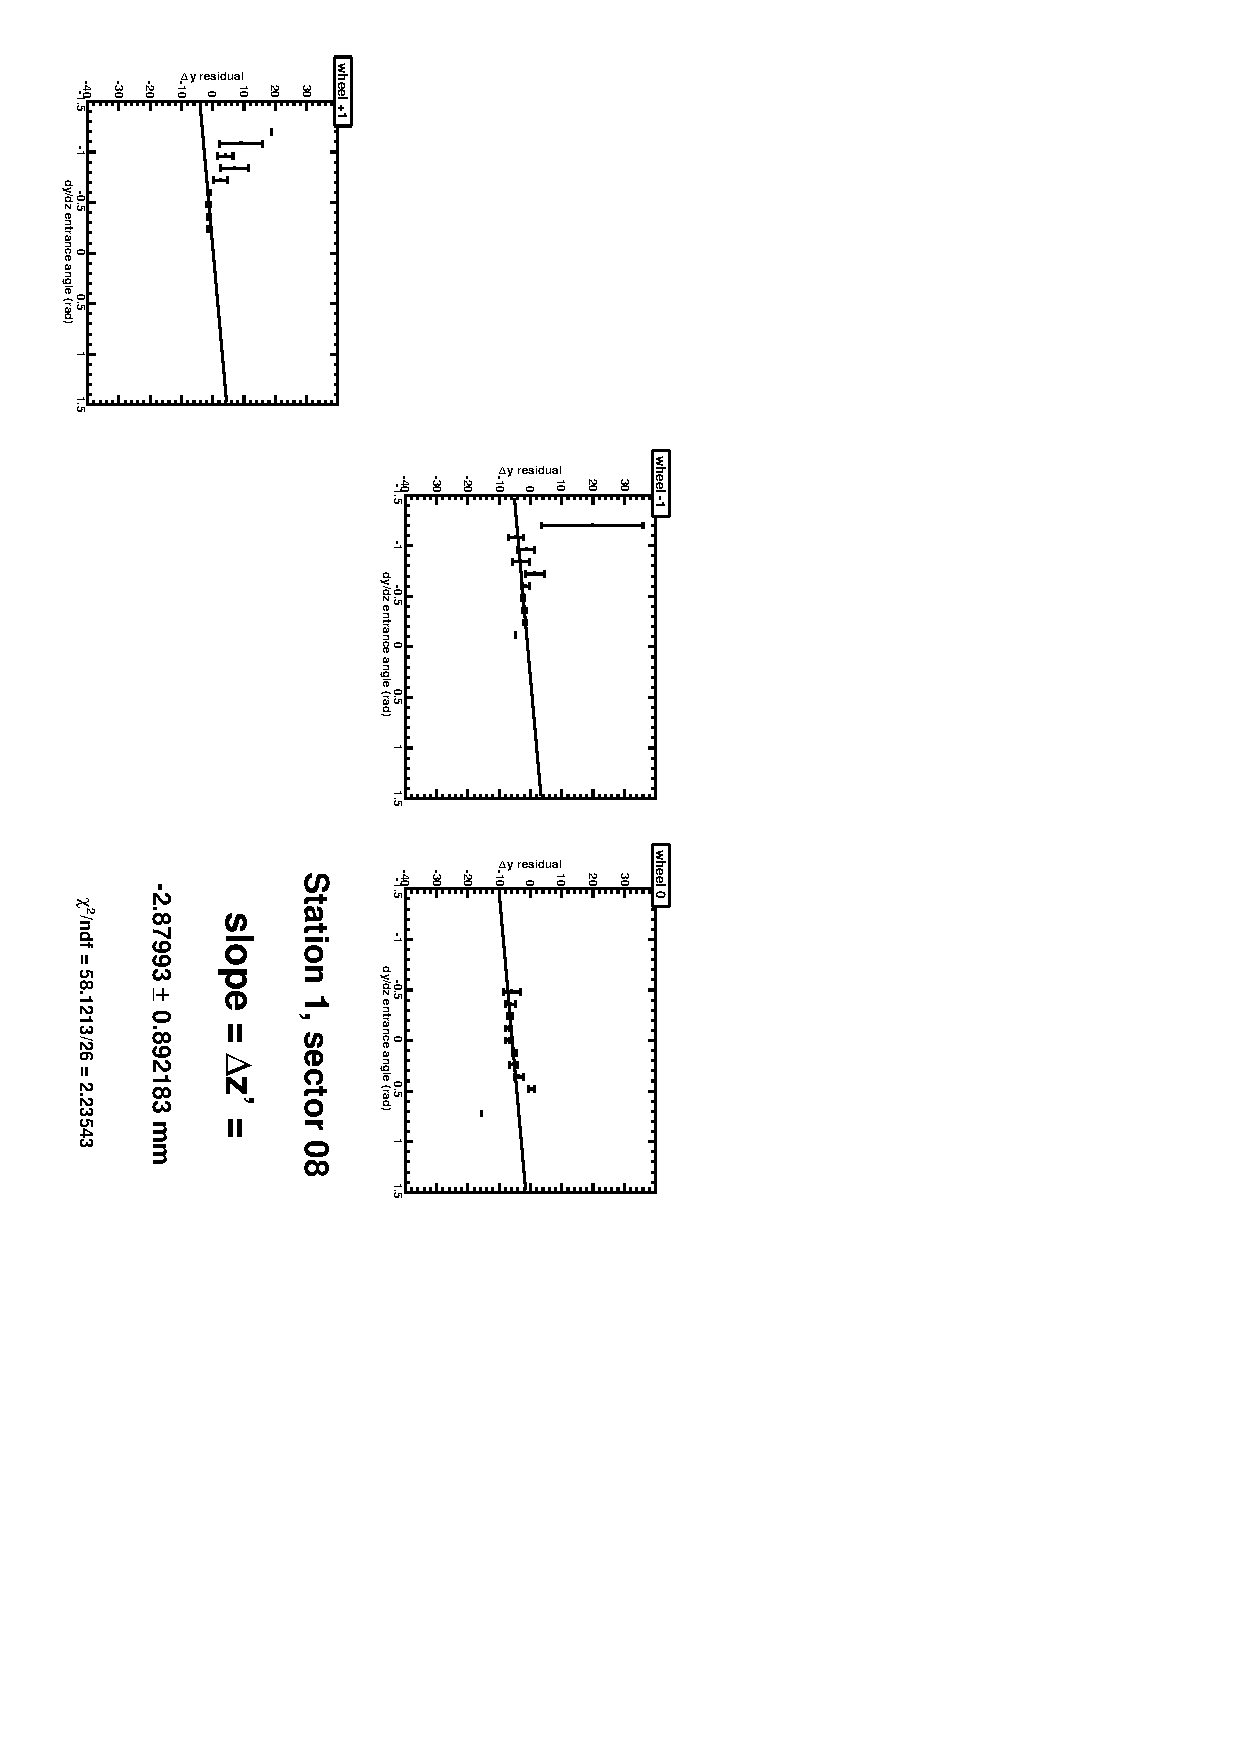
\includegraphics[height=\linewidth, angle=90]{zfits/zfit_1_08.pdf}

\vfill
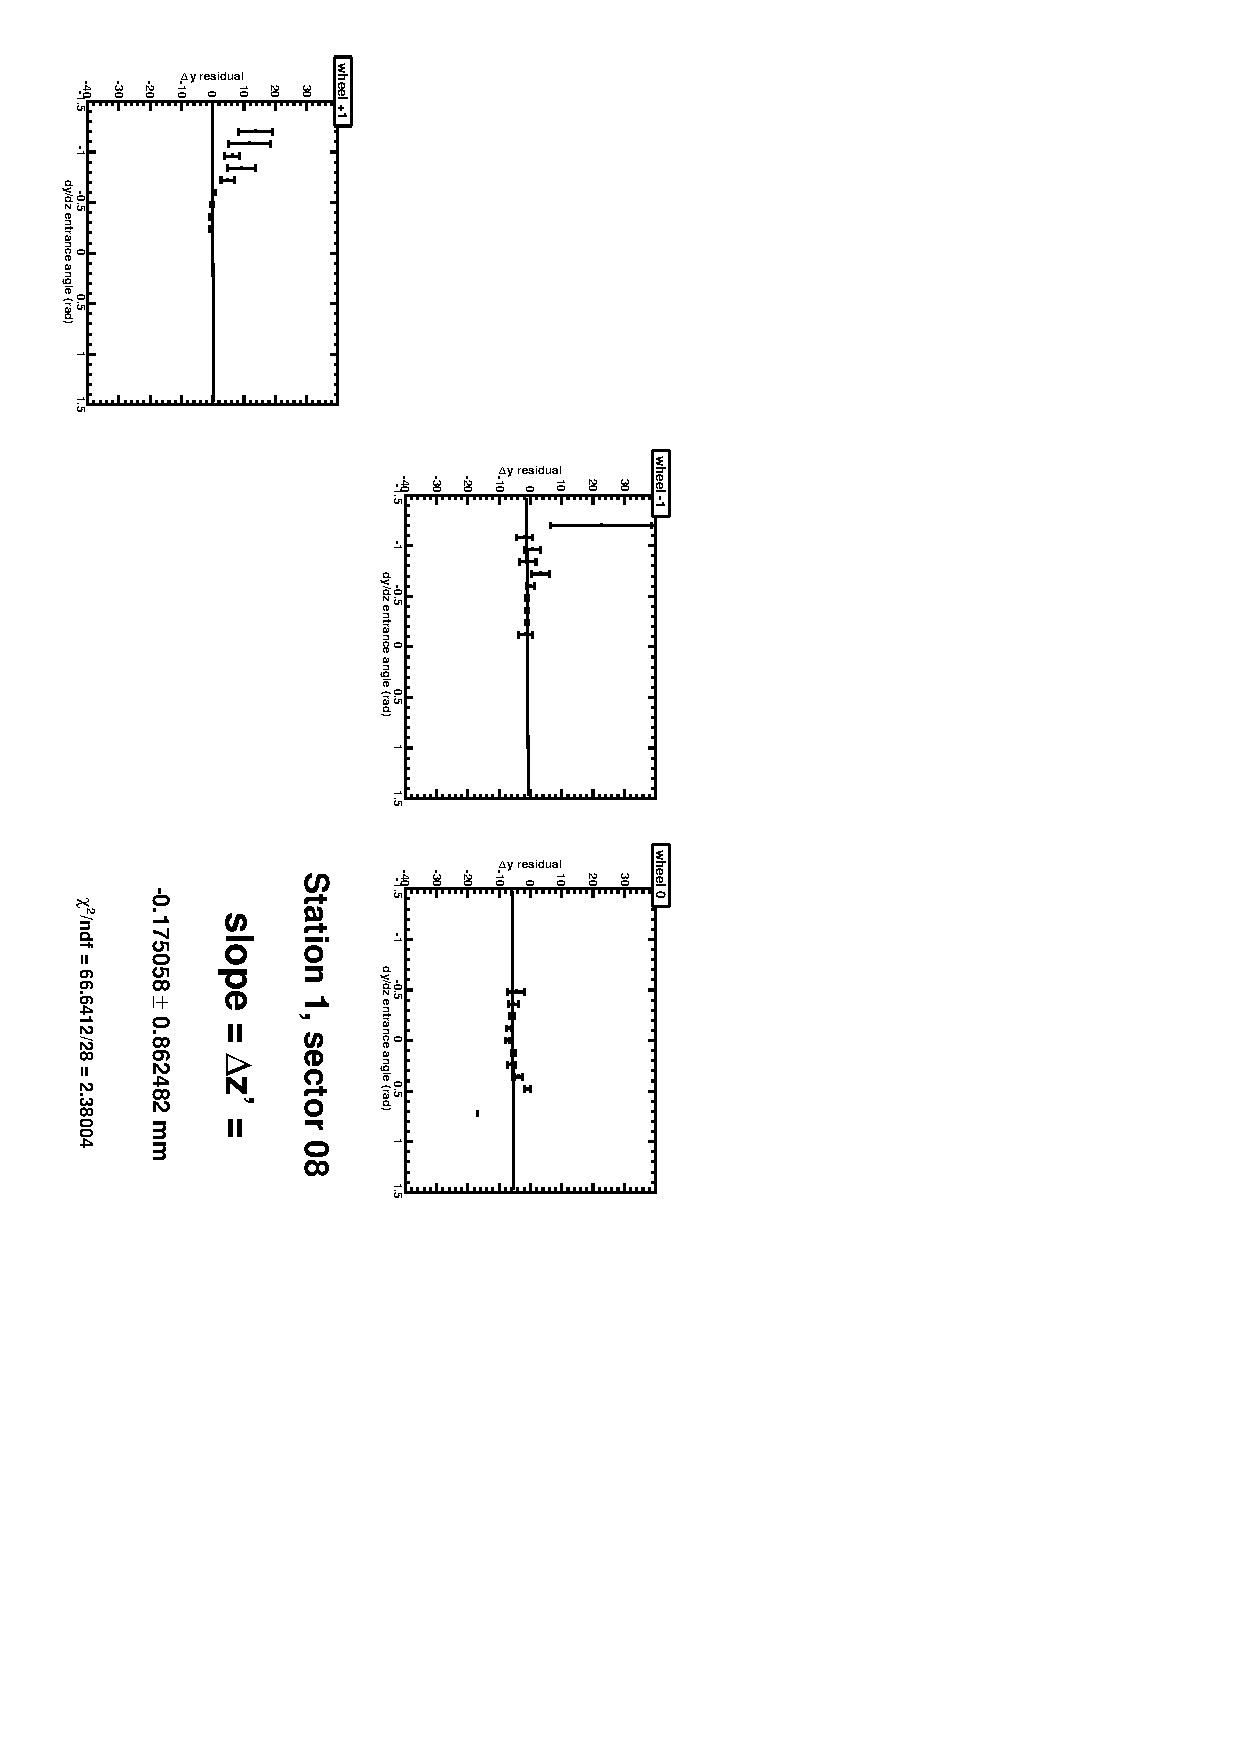
\includegraphics[height=\linewidth, angle=90]{zfits_after/zfit_1_08.pdf}
\column{0.3\linewidth}
\begin{itemize}
\item Top: before \\ Bottom: after
\item Five panels are wheels in the same SemiSuperSector (some are missing)
\item Fit requires all to have the same slope ($\delta_z$), but allows different offsets ($\delta_y$)
\end{itemize}
\end{columns}
\end{frame}

\begin{frame}
\frametitle{Station 1, sector 9}
\begin{columns}
\column{0.7\linewidth}
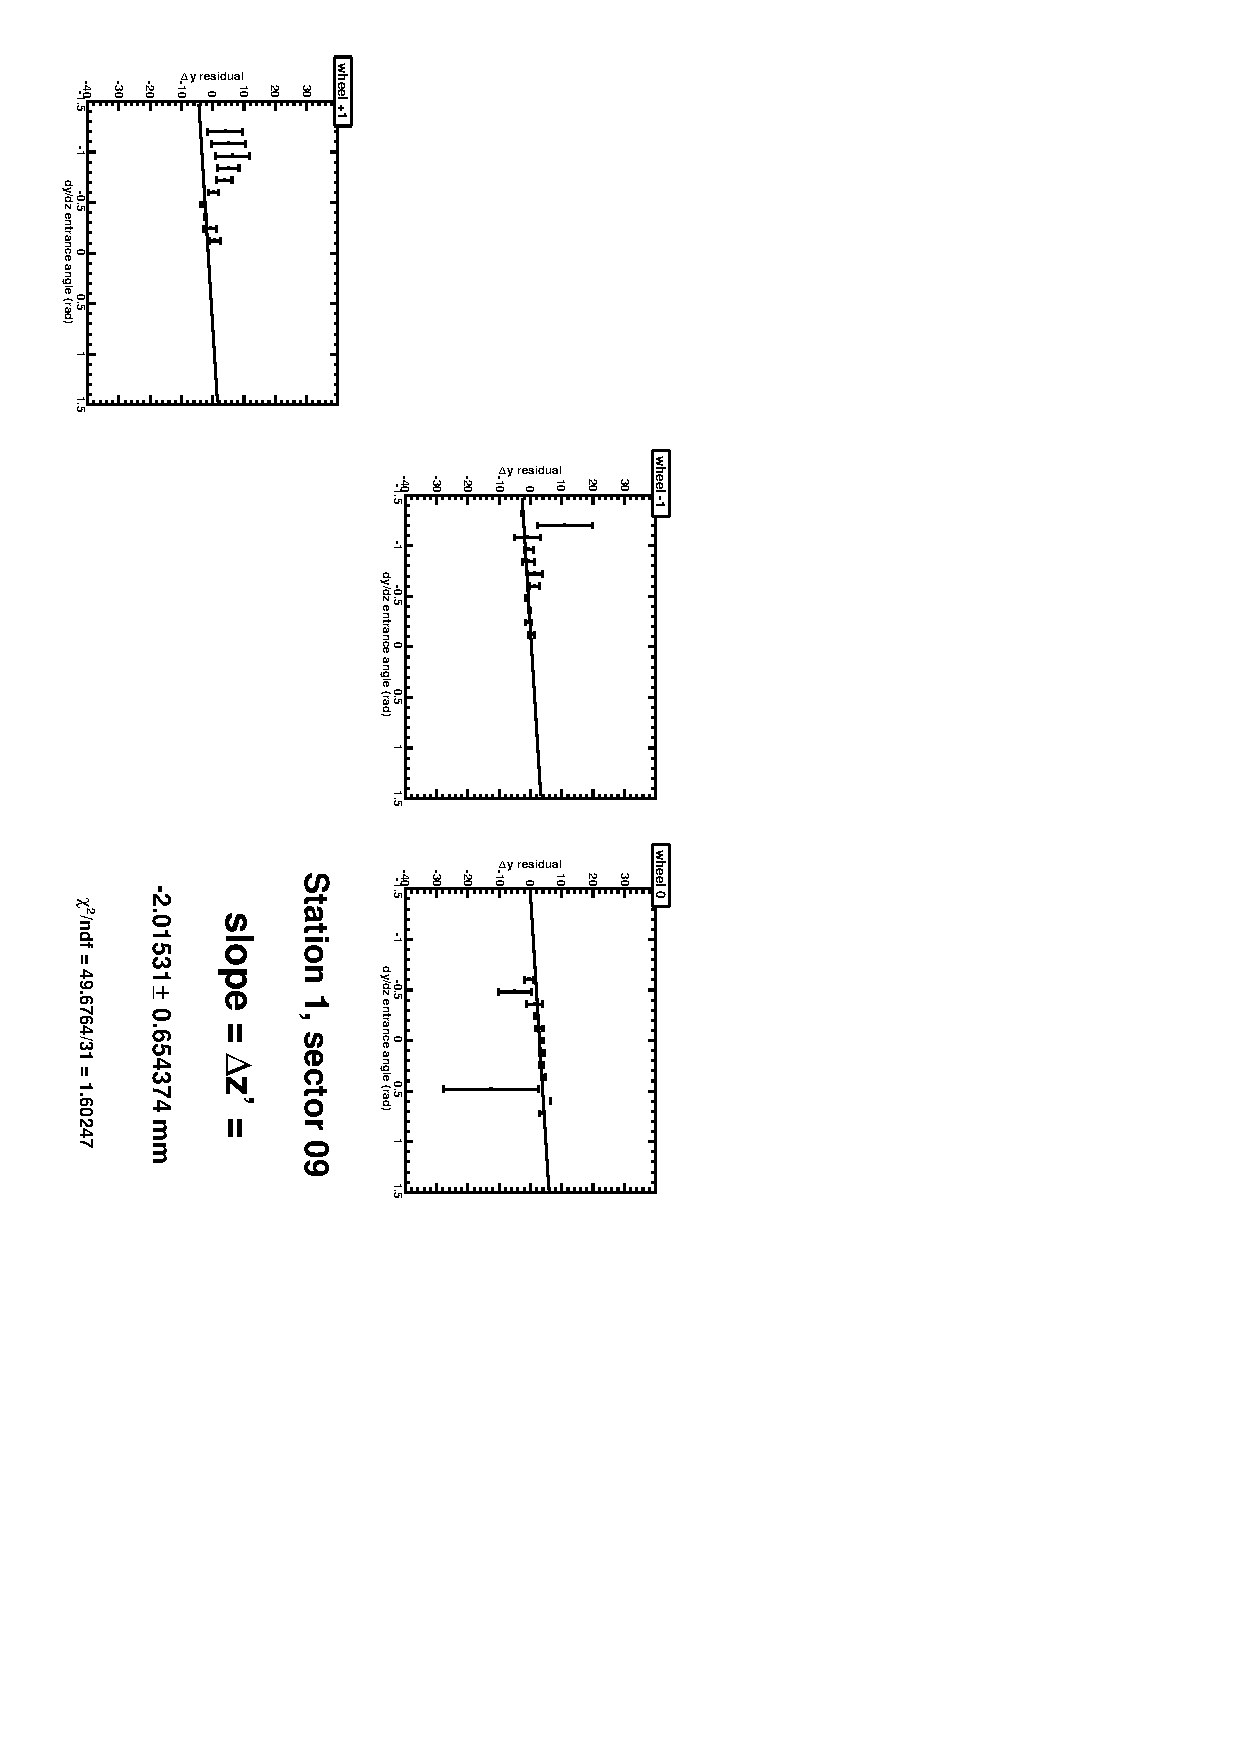
\includegraphics[height=\linewidth, angle=90]{zfits/zfit_1_09.pdf}

\vfill
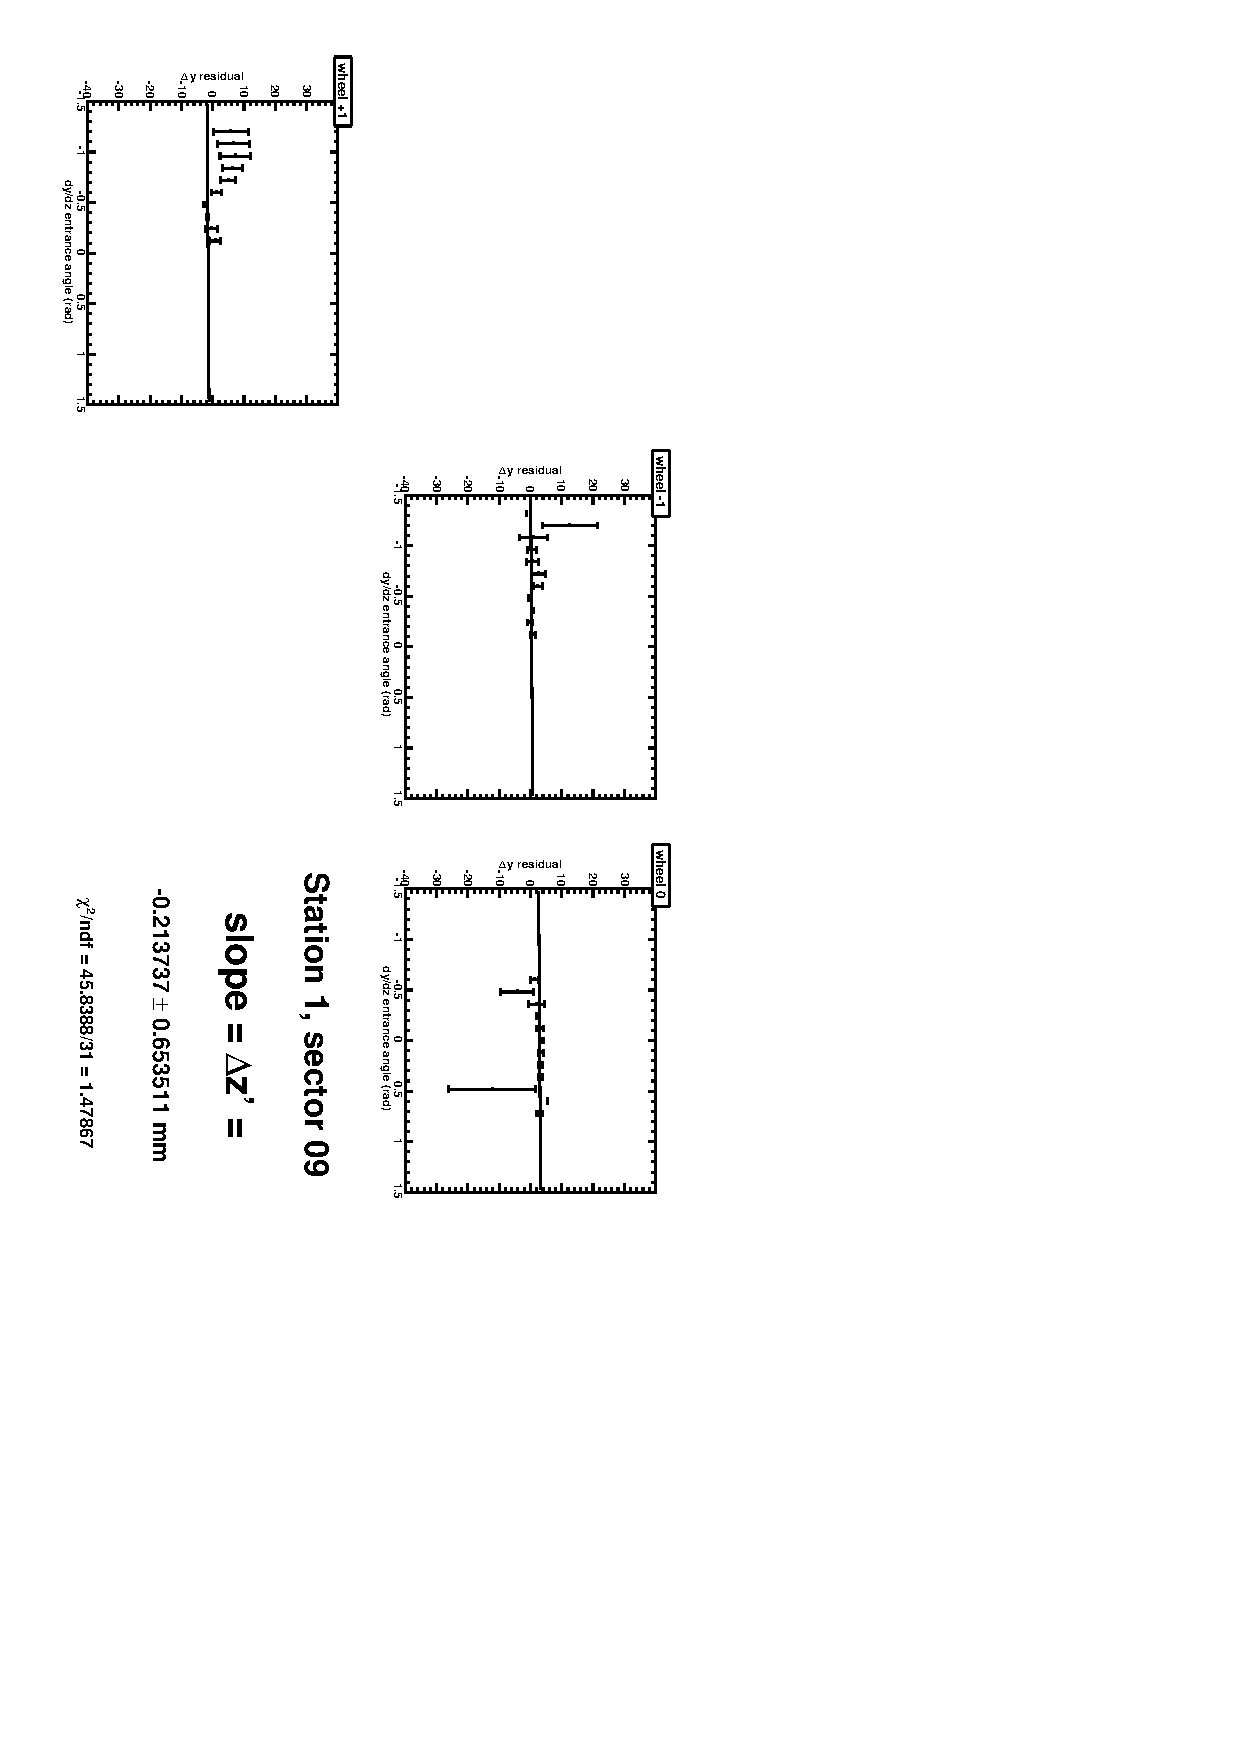
\includegraphics[height=\linewidth, angle=90]{zfits_after/zfit_1_09.pdf}
\column{0.3\linewidth}
\begin{itemize}
\item Top: before \\ Bottom: after
\item Five panels are wheels in the same SemiSuperSector (some are missing)
\item Fit requires all to have the same slope ($\delta_z$), but allows different offsets ($\delta_y$)
\end{itemize}
\end{columns}
\end{frame}

\begin{frame}
\frametitle{Station 1, sector 10}
\begin{columns}
\column{0.7\linewidth}
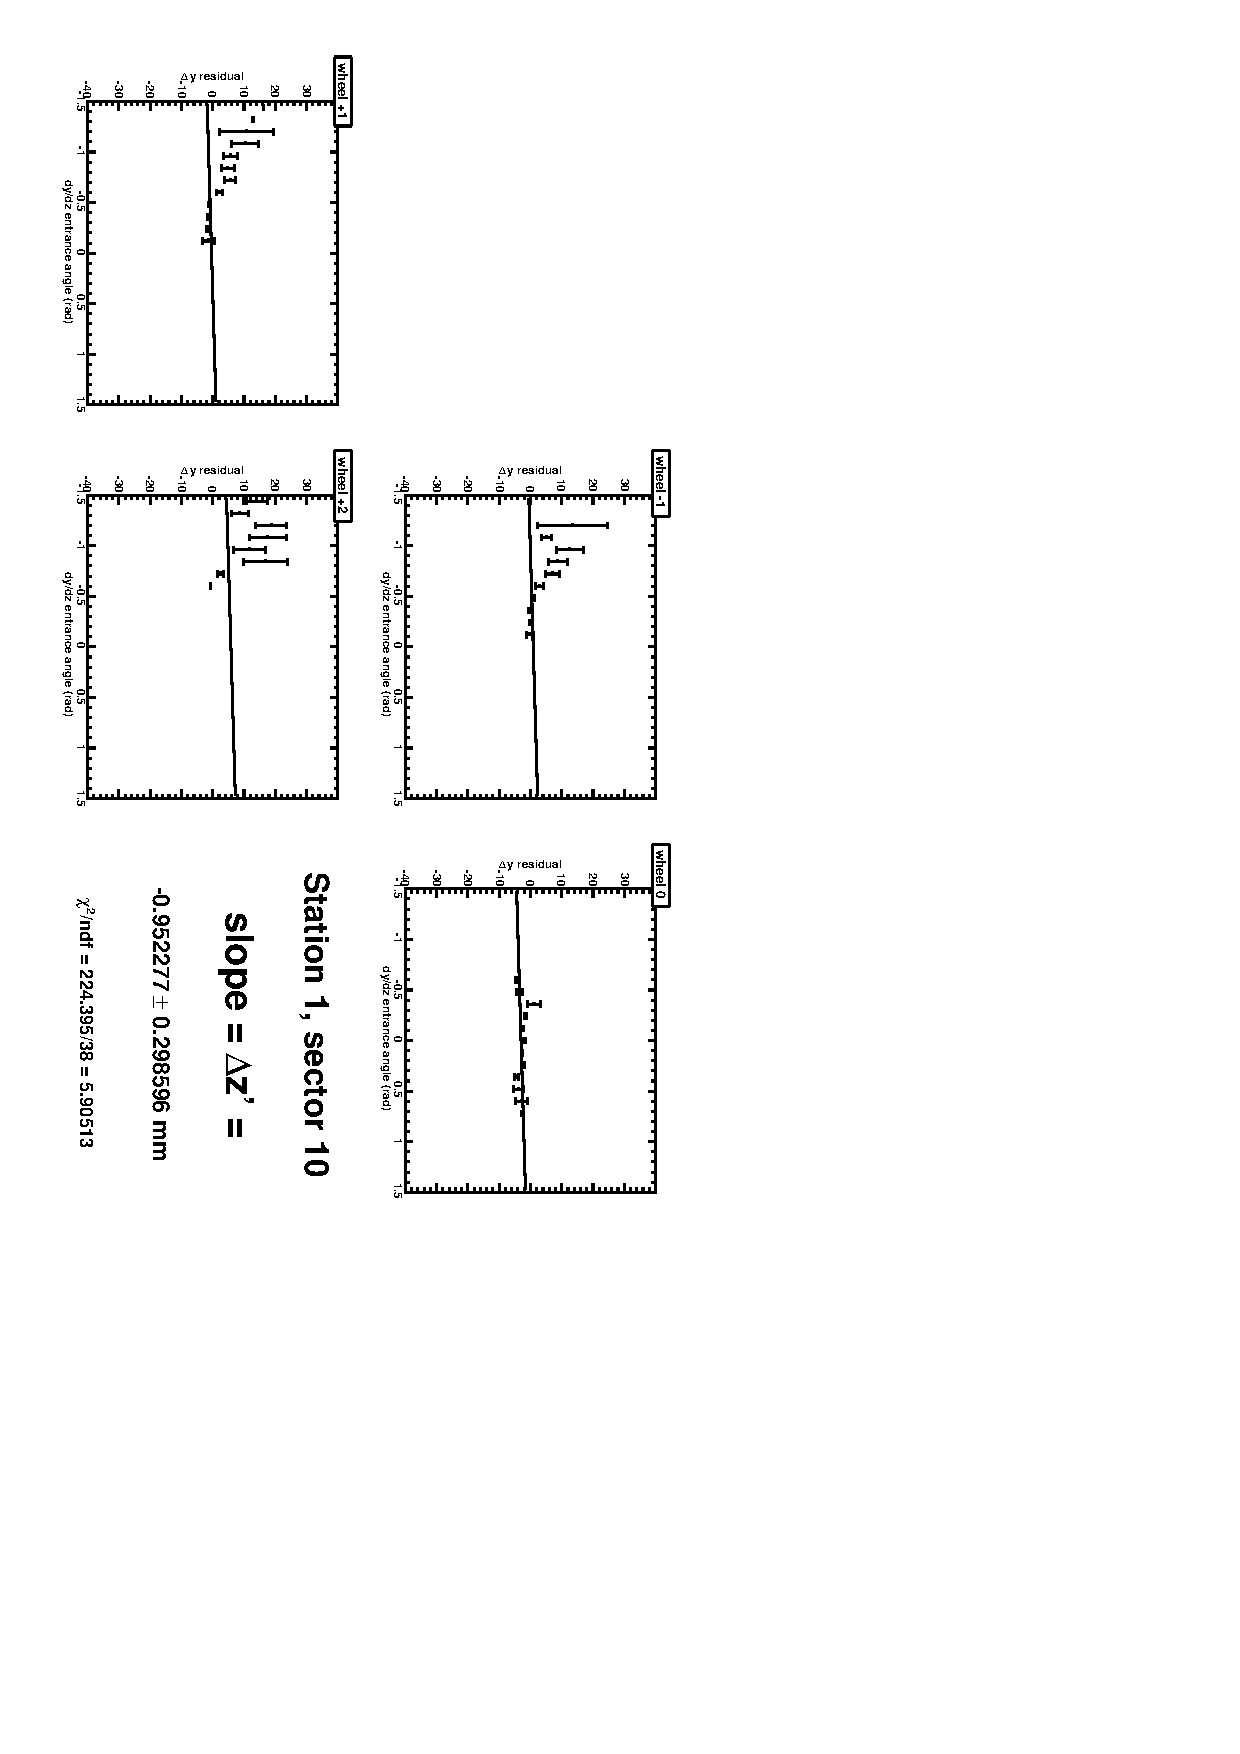
\includegraphics[height=\linewidth, angle=90]{zfits/zfit_1_10.pdf}

\vfill
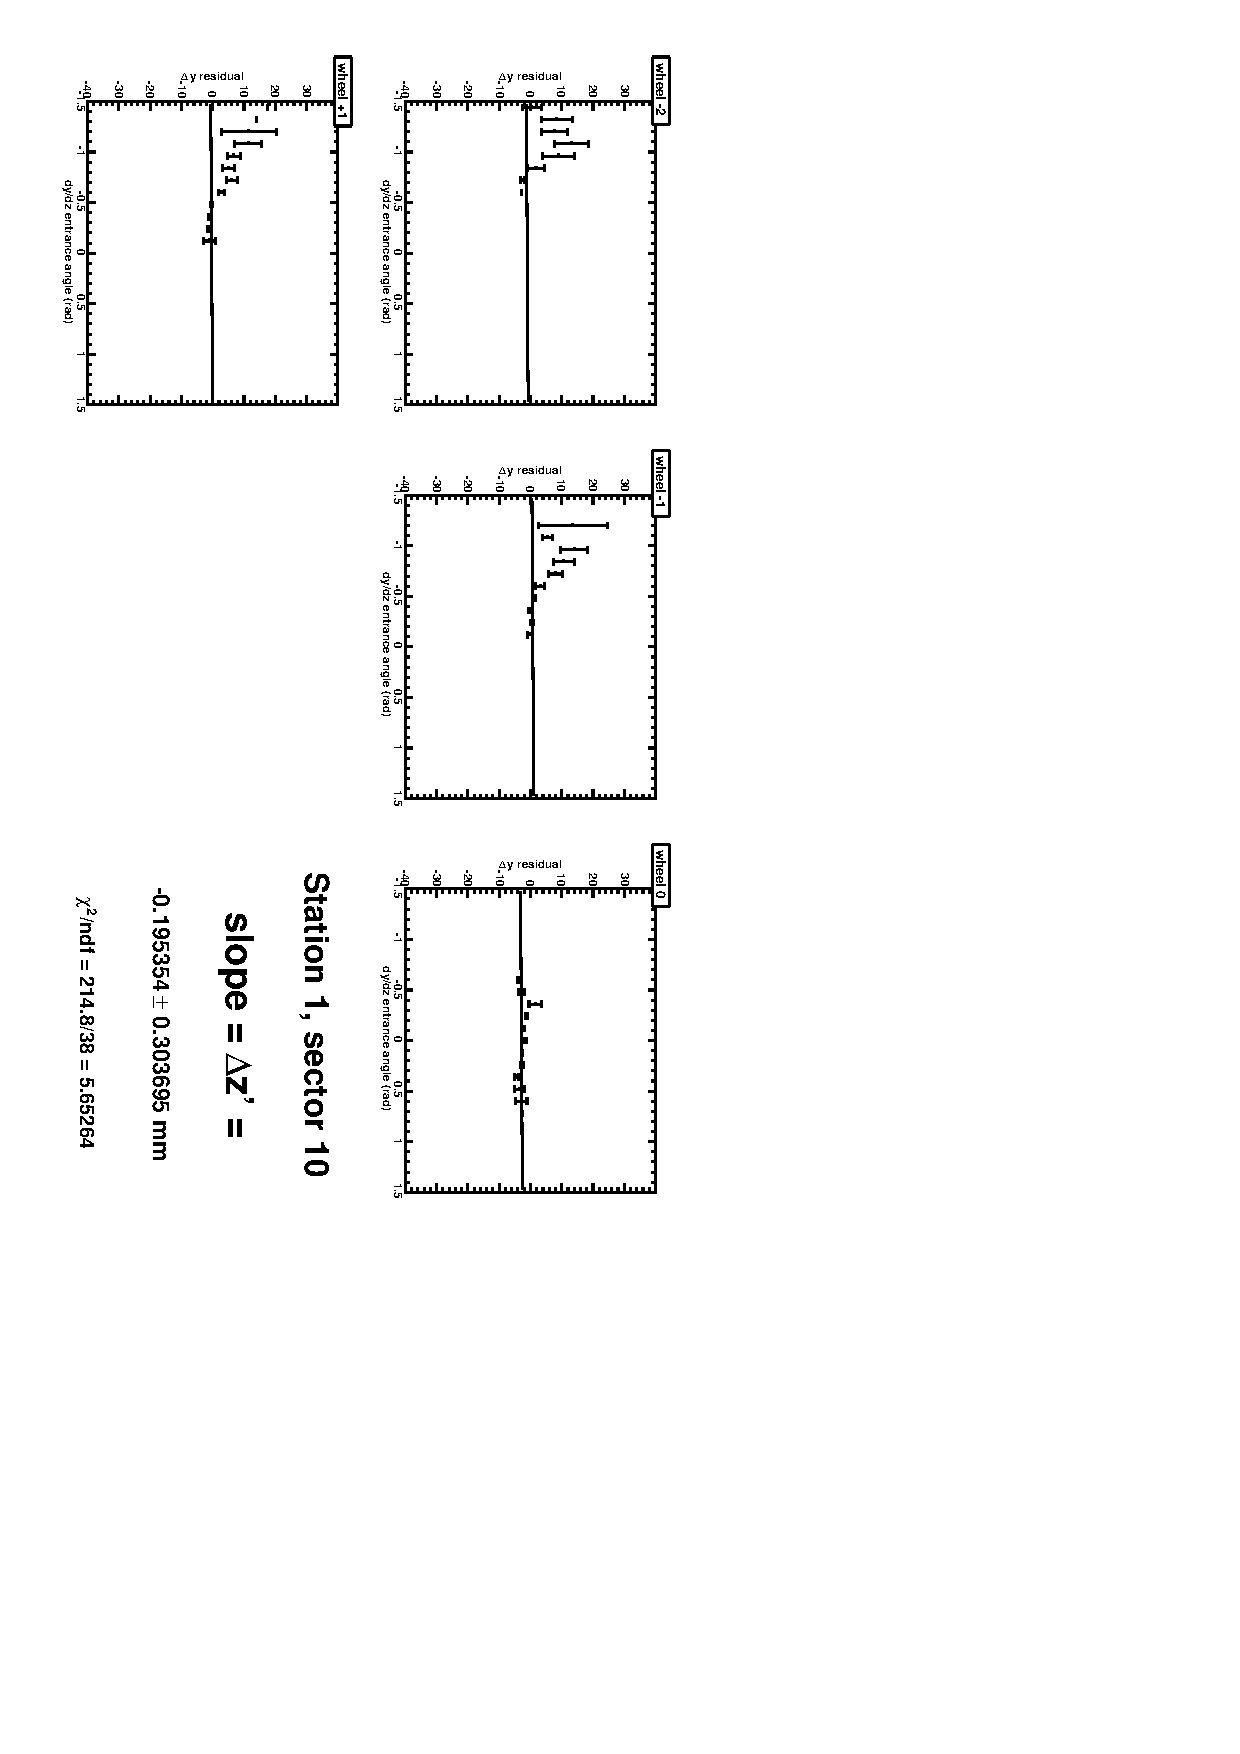
\includegraphics[height=\linewidth, angle=90]{zfits_after/zfit_1_10.pdf}
\column{0.3\linewidth}
\begin{itemize}
\item Top: before \\ Bottom: after
\item Five panels are wheels in the same SemiSuperSector (some are missing)
\item Fit requires all to have the same slope ($\delta_z$), but allows different offsets ($\delta_y$)
\end{itemize}
\end{columns}
\end{frame}

\begin{frame}
\frametitle{Station 1, sector 11}
\begin{columns}
\column{0.7\linewidth}
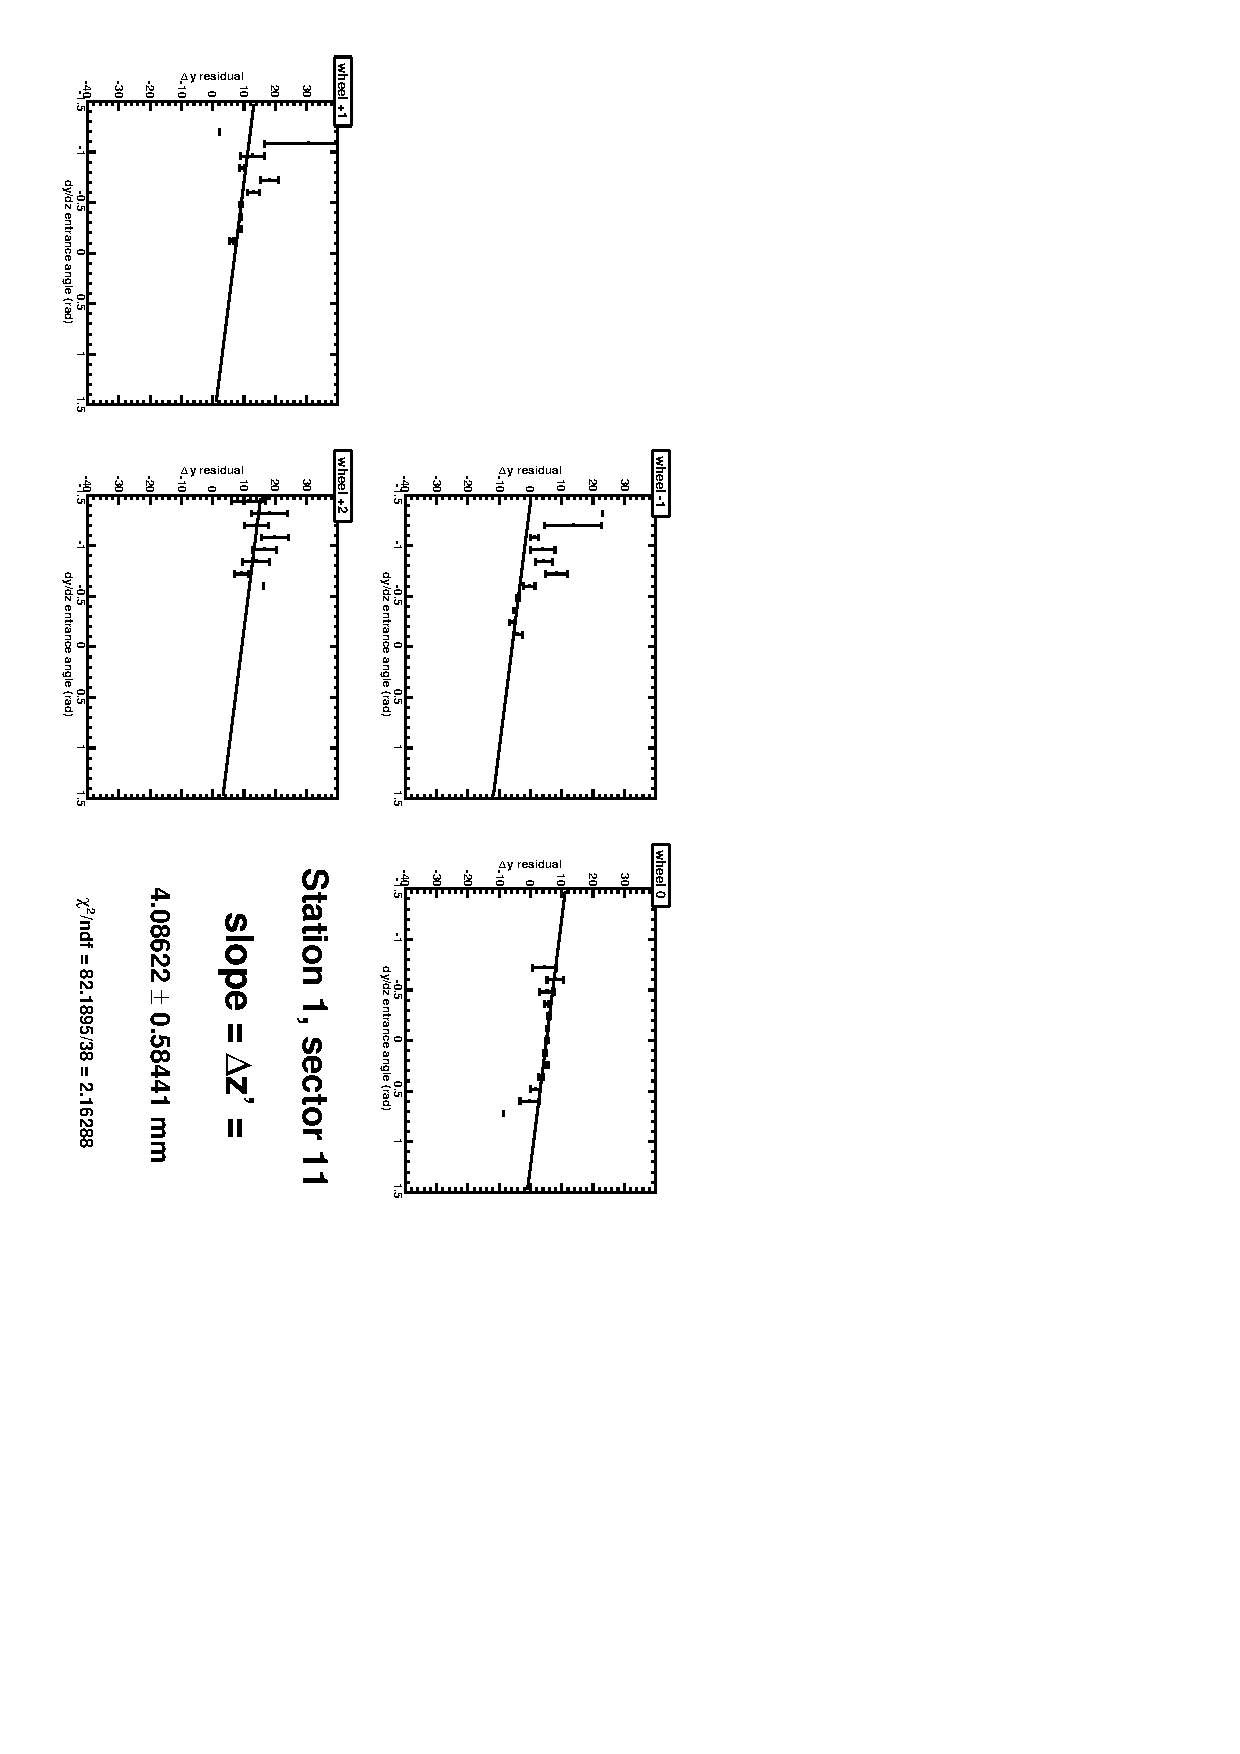
\includegraphics[height=\linewidth, angle=90]{zfits/zfit_1_11.pdf}

\vfill
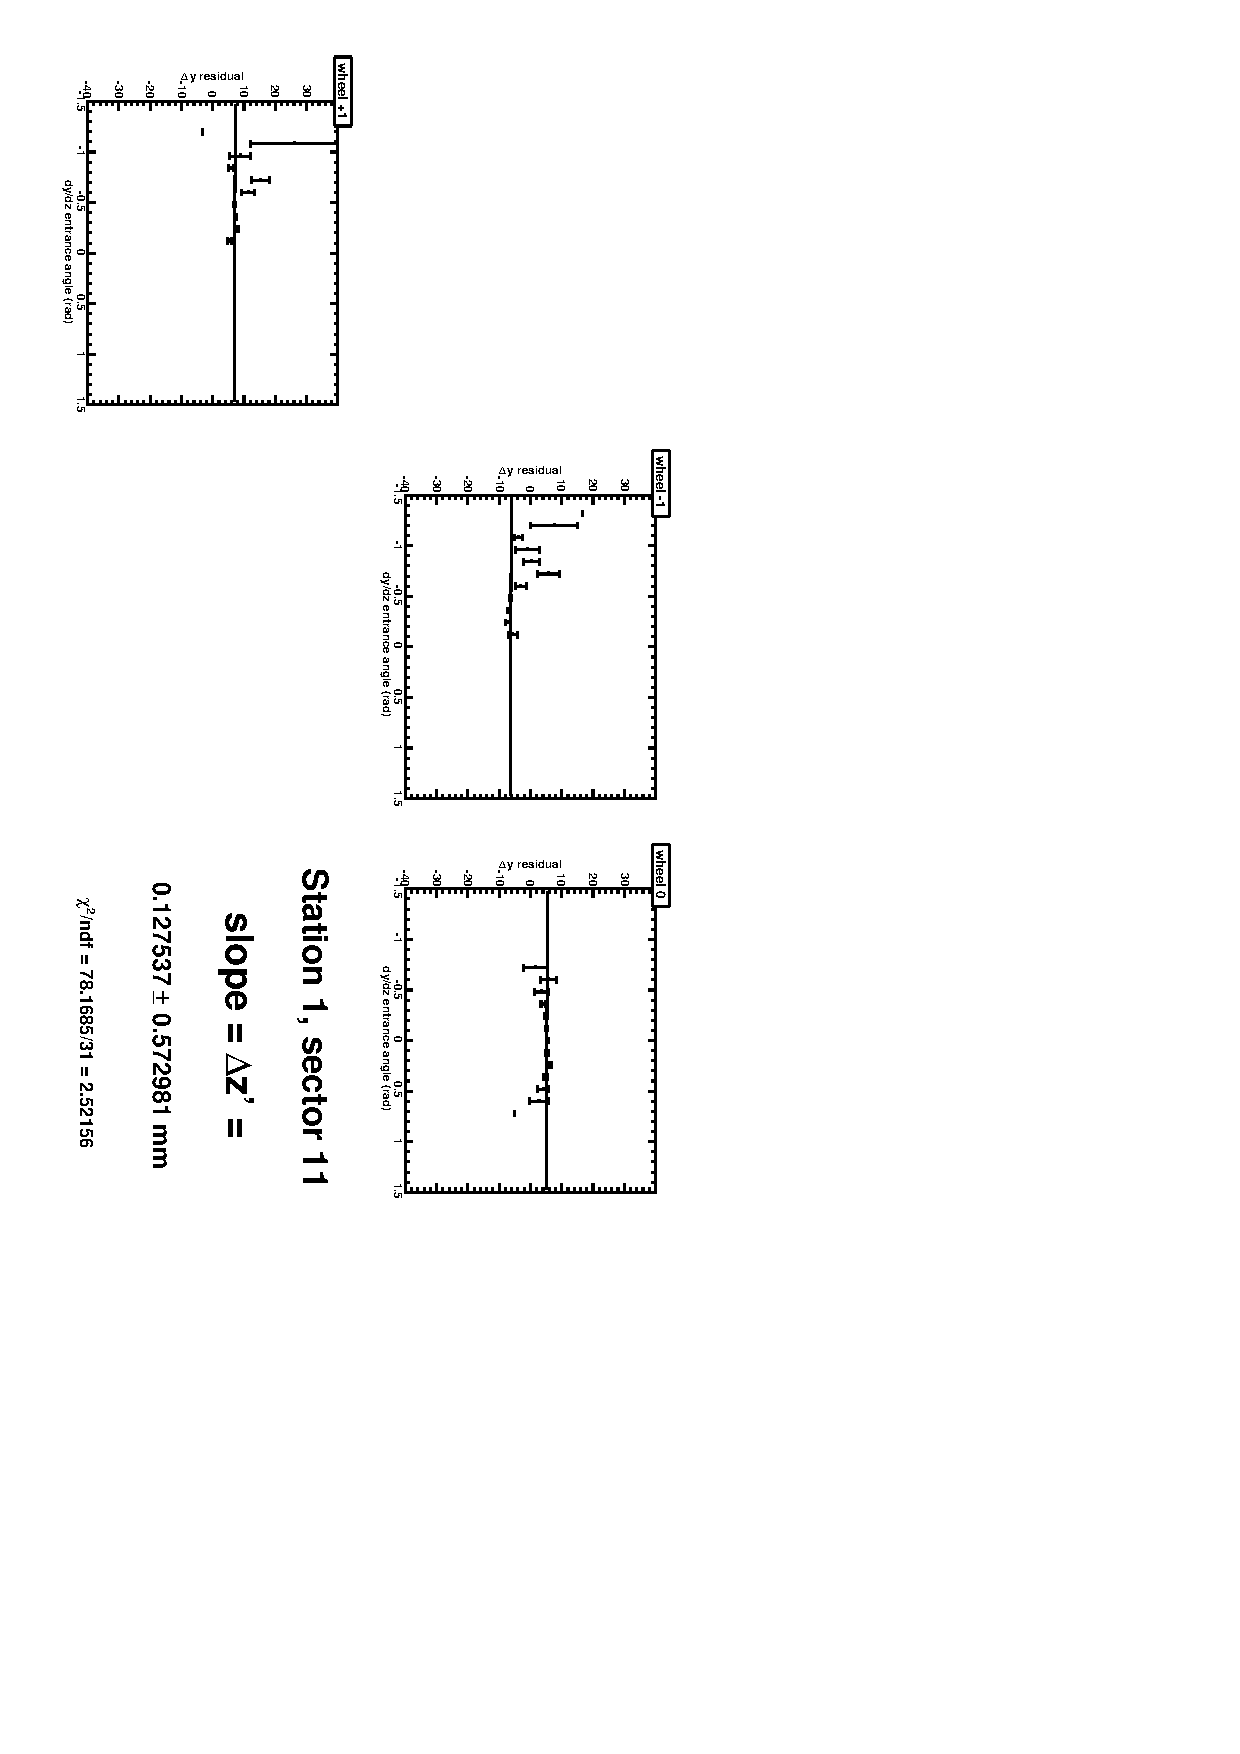
\includegraphics[height=\linewidth, angle=90]{zfits_after/zfit_1_11.pdf}
\column{0.3\linewidth}
\begin{itemize}
\item Top: before \\ Bottom: after
\item Five panels are wheels in the same SemiSuperSector (some are missing)
\item Fit requires all to have the same slope ($\delta_z$), but allows different offsets ($\delta_y$)
\end{itemize}
\end{columns}
\end{frame}

\begin{frame}
\frametitle{Station 1, sector 12}
\begin{columns}
\column{0.7\linewidth}
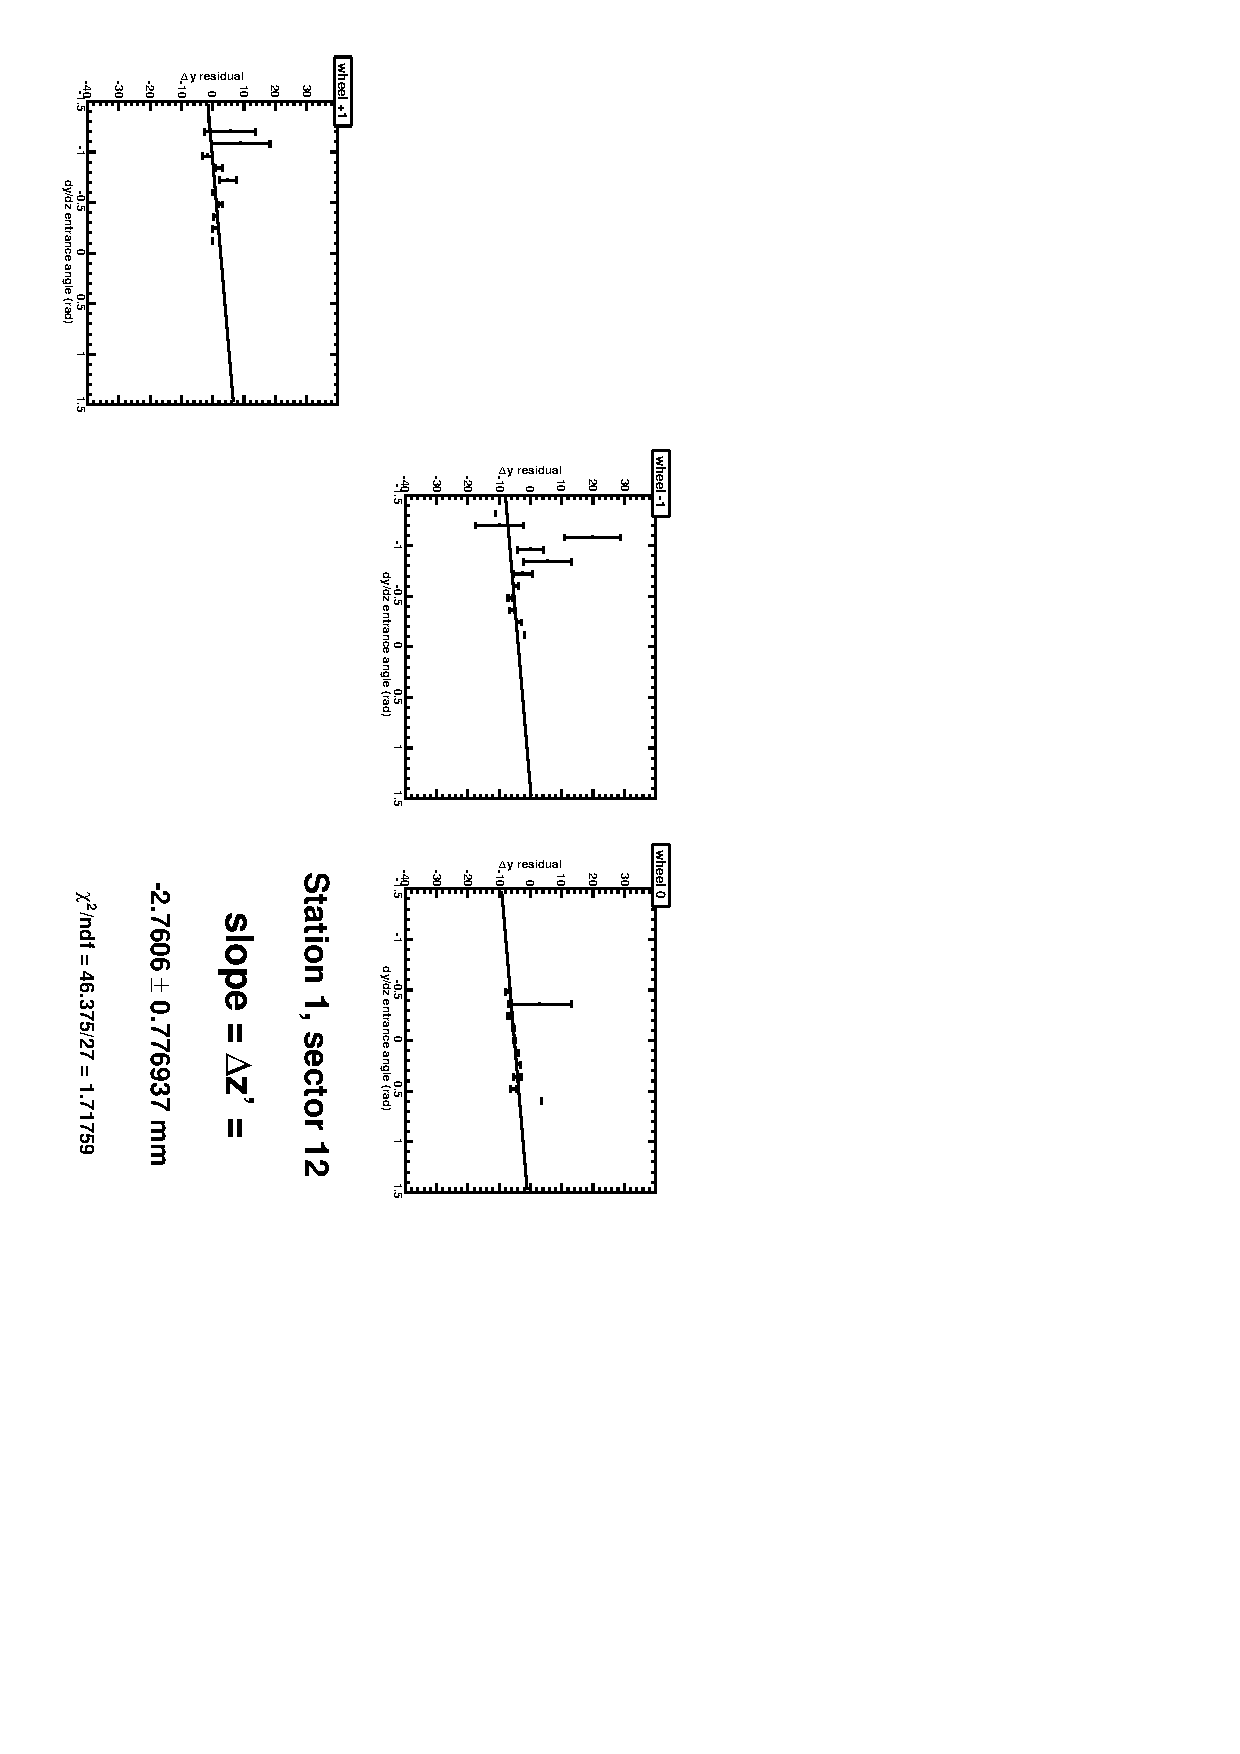
\includegraphics[height=\linewidth, angle=90]{zfits/zfit_1_12.pdf}

\vfill
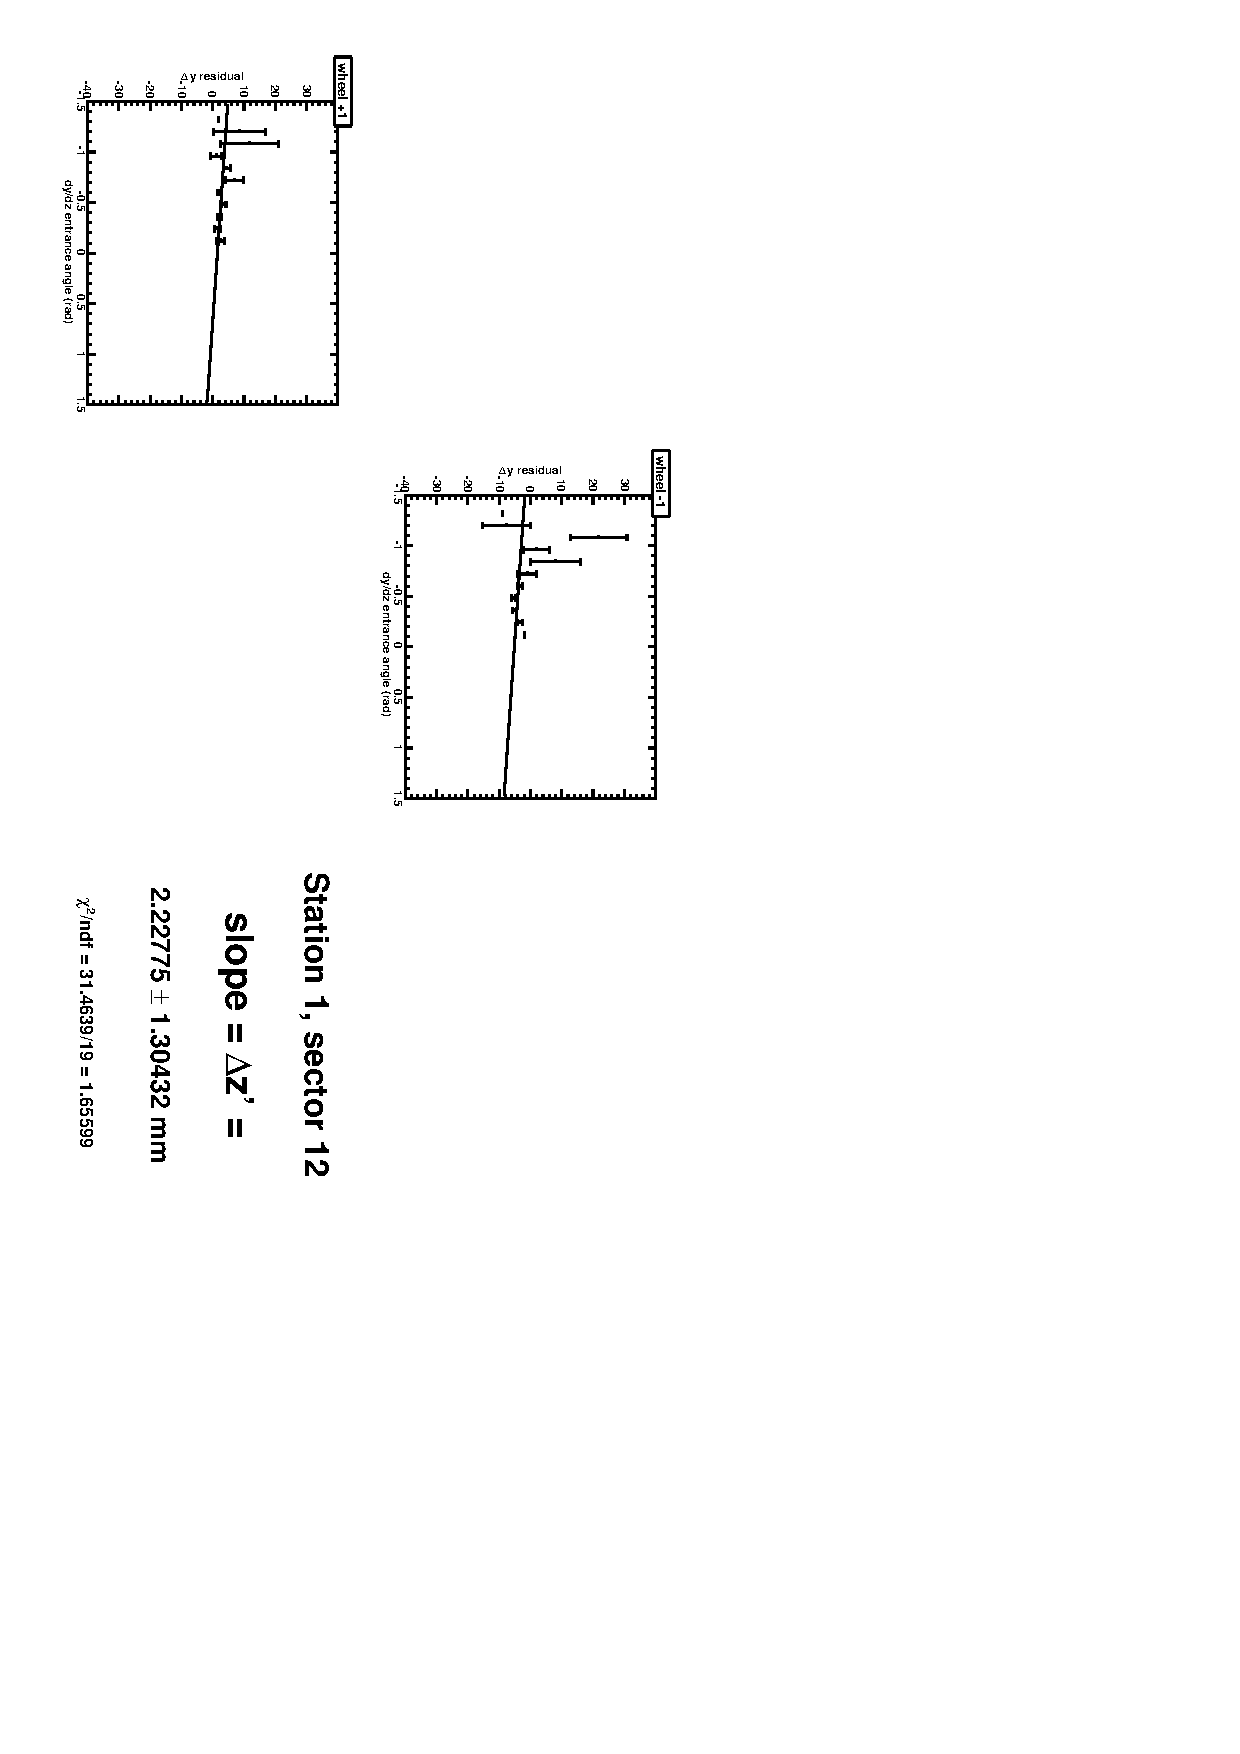
\includegraphics[height=\linewidth, angle=90]{zfits_after/zfit_1_12.pdf}
\column{0.3\linewidth}
\begin{itemize}
\item Top: before \\ Bottom: after
\item Five panels are wheels in the same SemiSuperSector (some are missing)
\item Fit requires all to have the same slope ($\delta_z$), but allows different offsets ($\delta_y$)
\end{itemize}
\end{columns}
\end{frame}

\begin{frame}
\frametitle{Station 2, sector 1}
\begin{columns}
\column{0.7\linewidth}
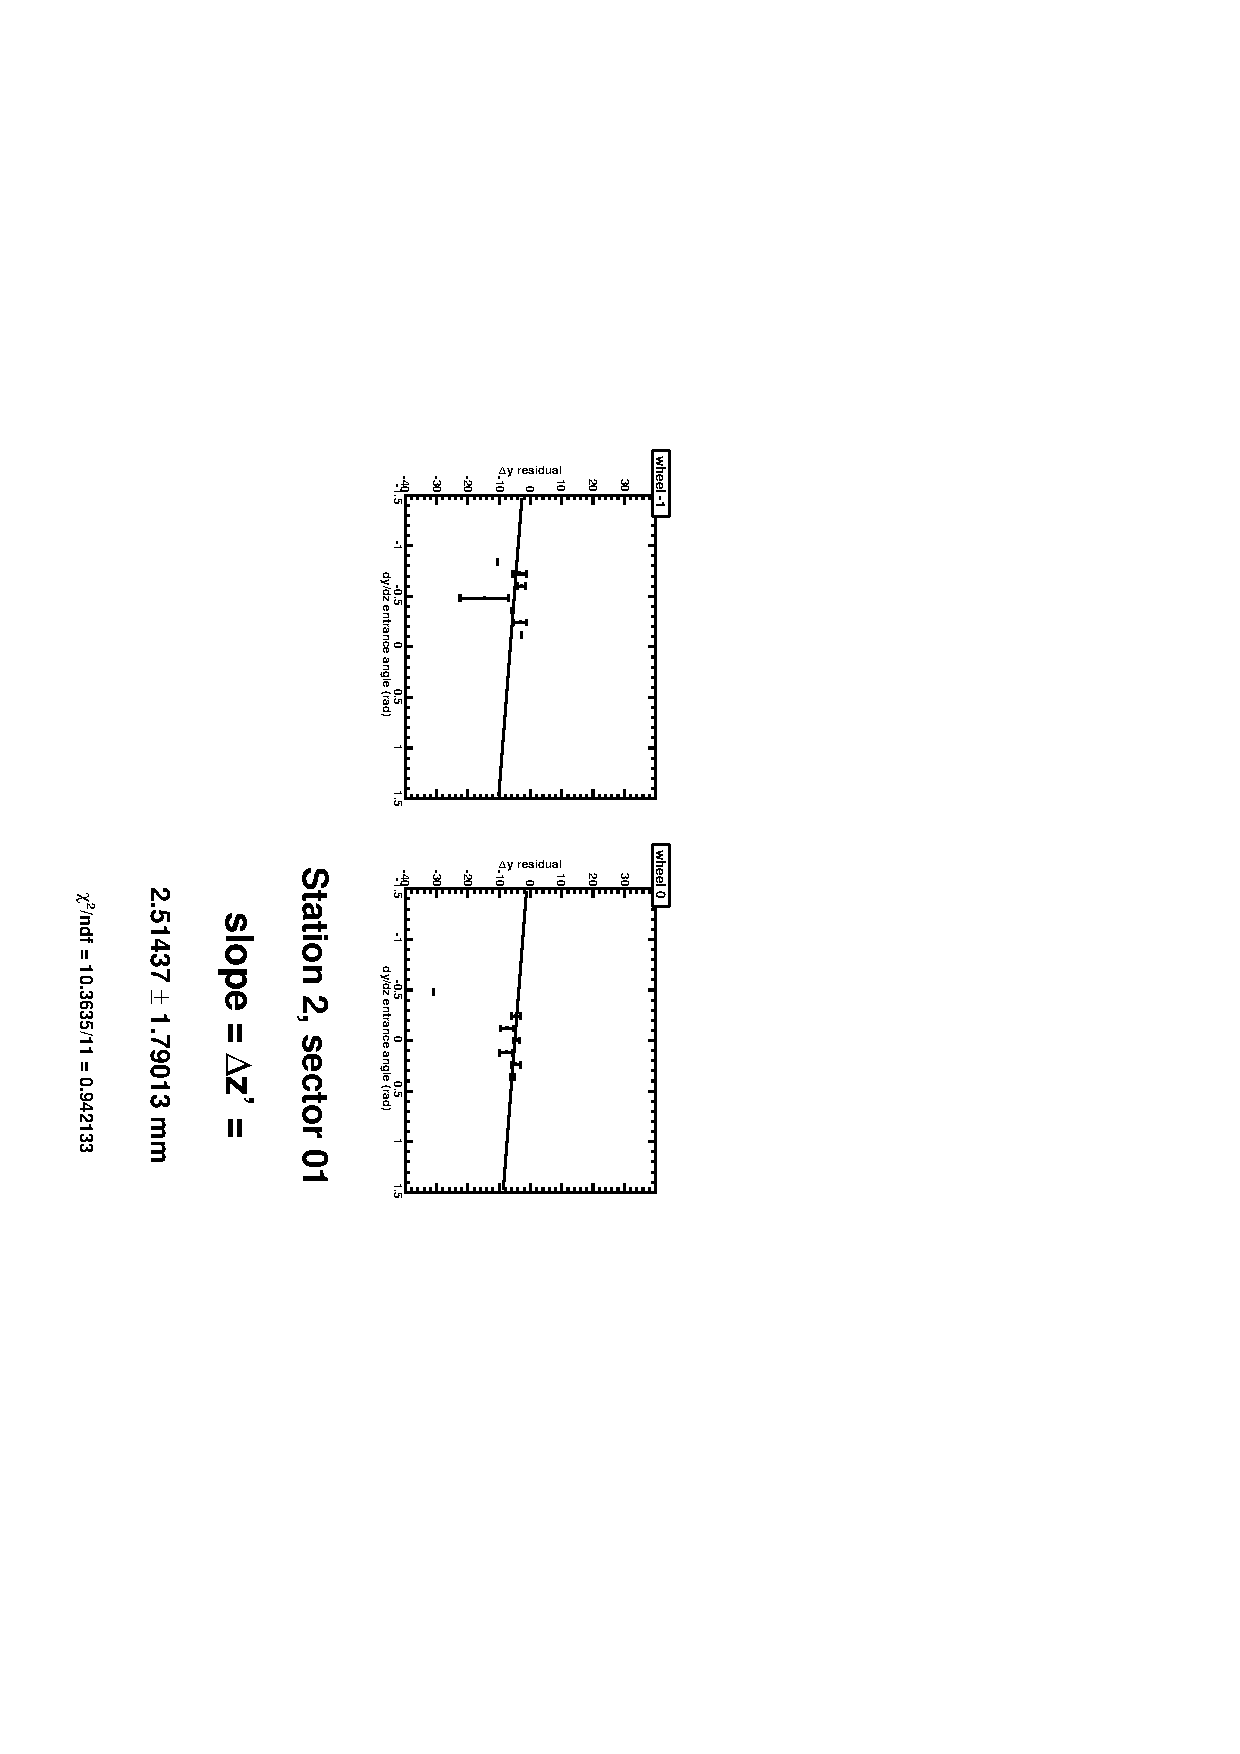
\includegraphics[height=\linewidth, angle=90]{zfits/zfit_2_01.pdf}

\vfill
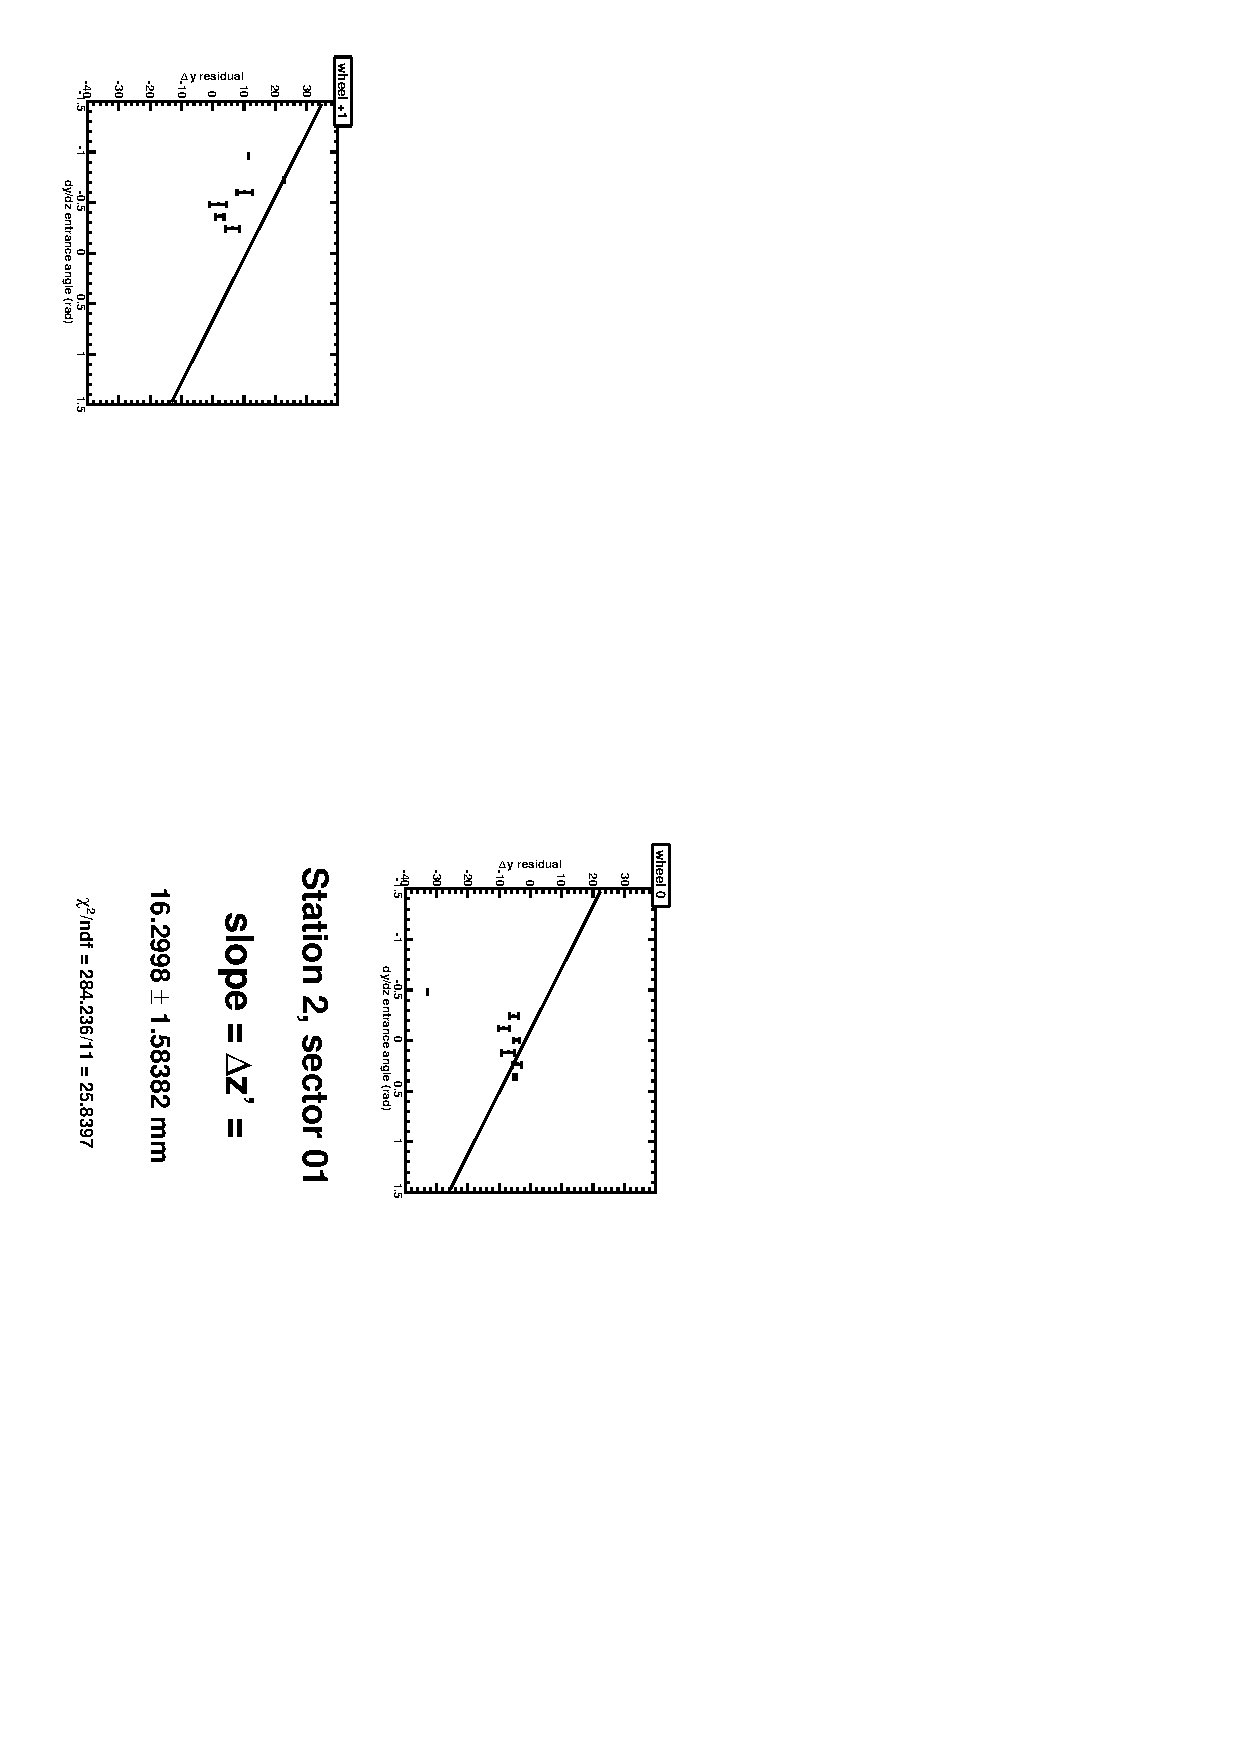
\includegraphics[height=\linewidth, angle=90]{zfits_after/zfit_2_01.pdf}
\column{0.3\linewidth}
\begin{itemize}
\item Top: before \\ Bottom: after
\item Five panels are wheels in the same SemiSuperSector (some are missing)
\item Fit requires all to have the same slope ($\delta_z$), but allows different offsets ($\delta_y$)
\end{itemize}
\end{columns}
\end{frame}

\begin{frame}
\frametitle{Station 2, sector 2}
\begin{columns}
\column{0.7\linewidth}
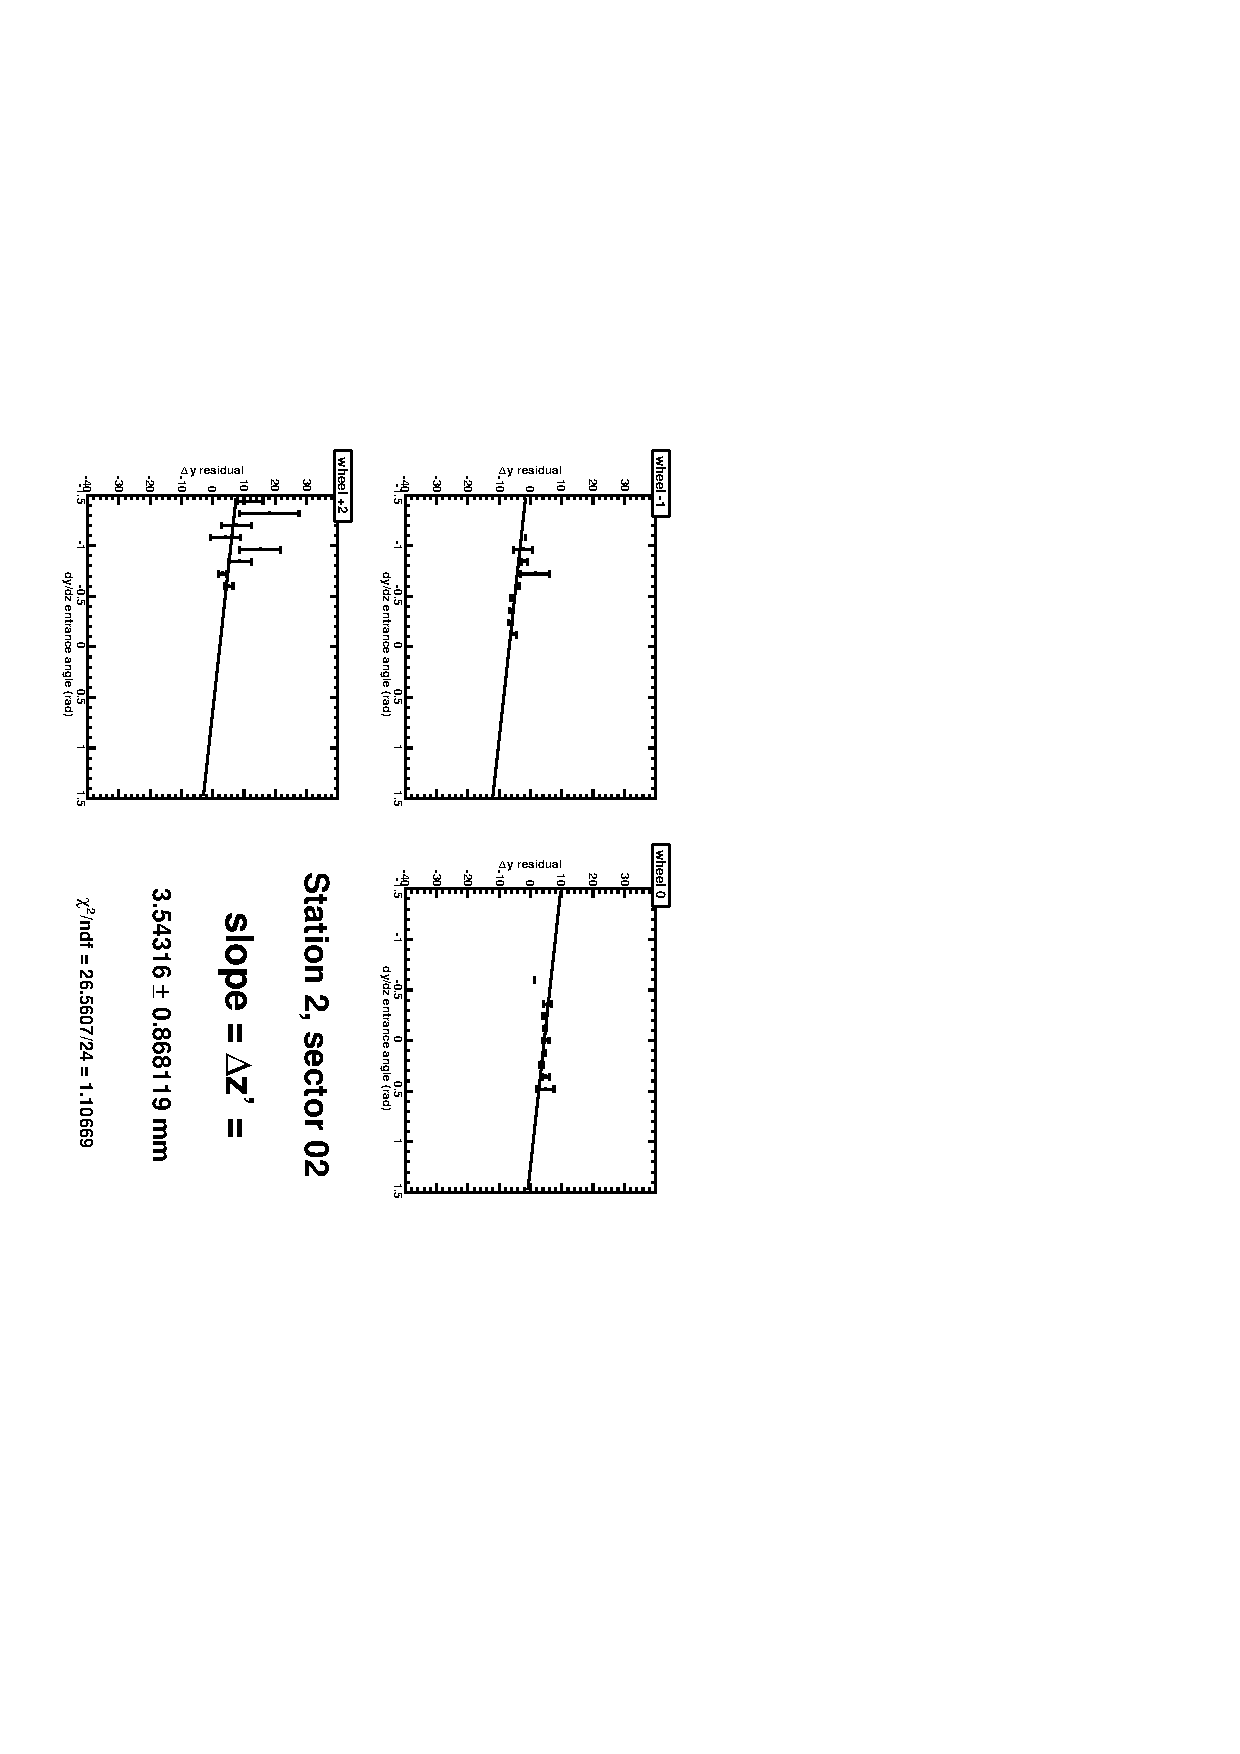
\includegraphics[height=\linewidth, angle=90]{zfits/zfit_2_02.pdf}

\vfill
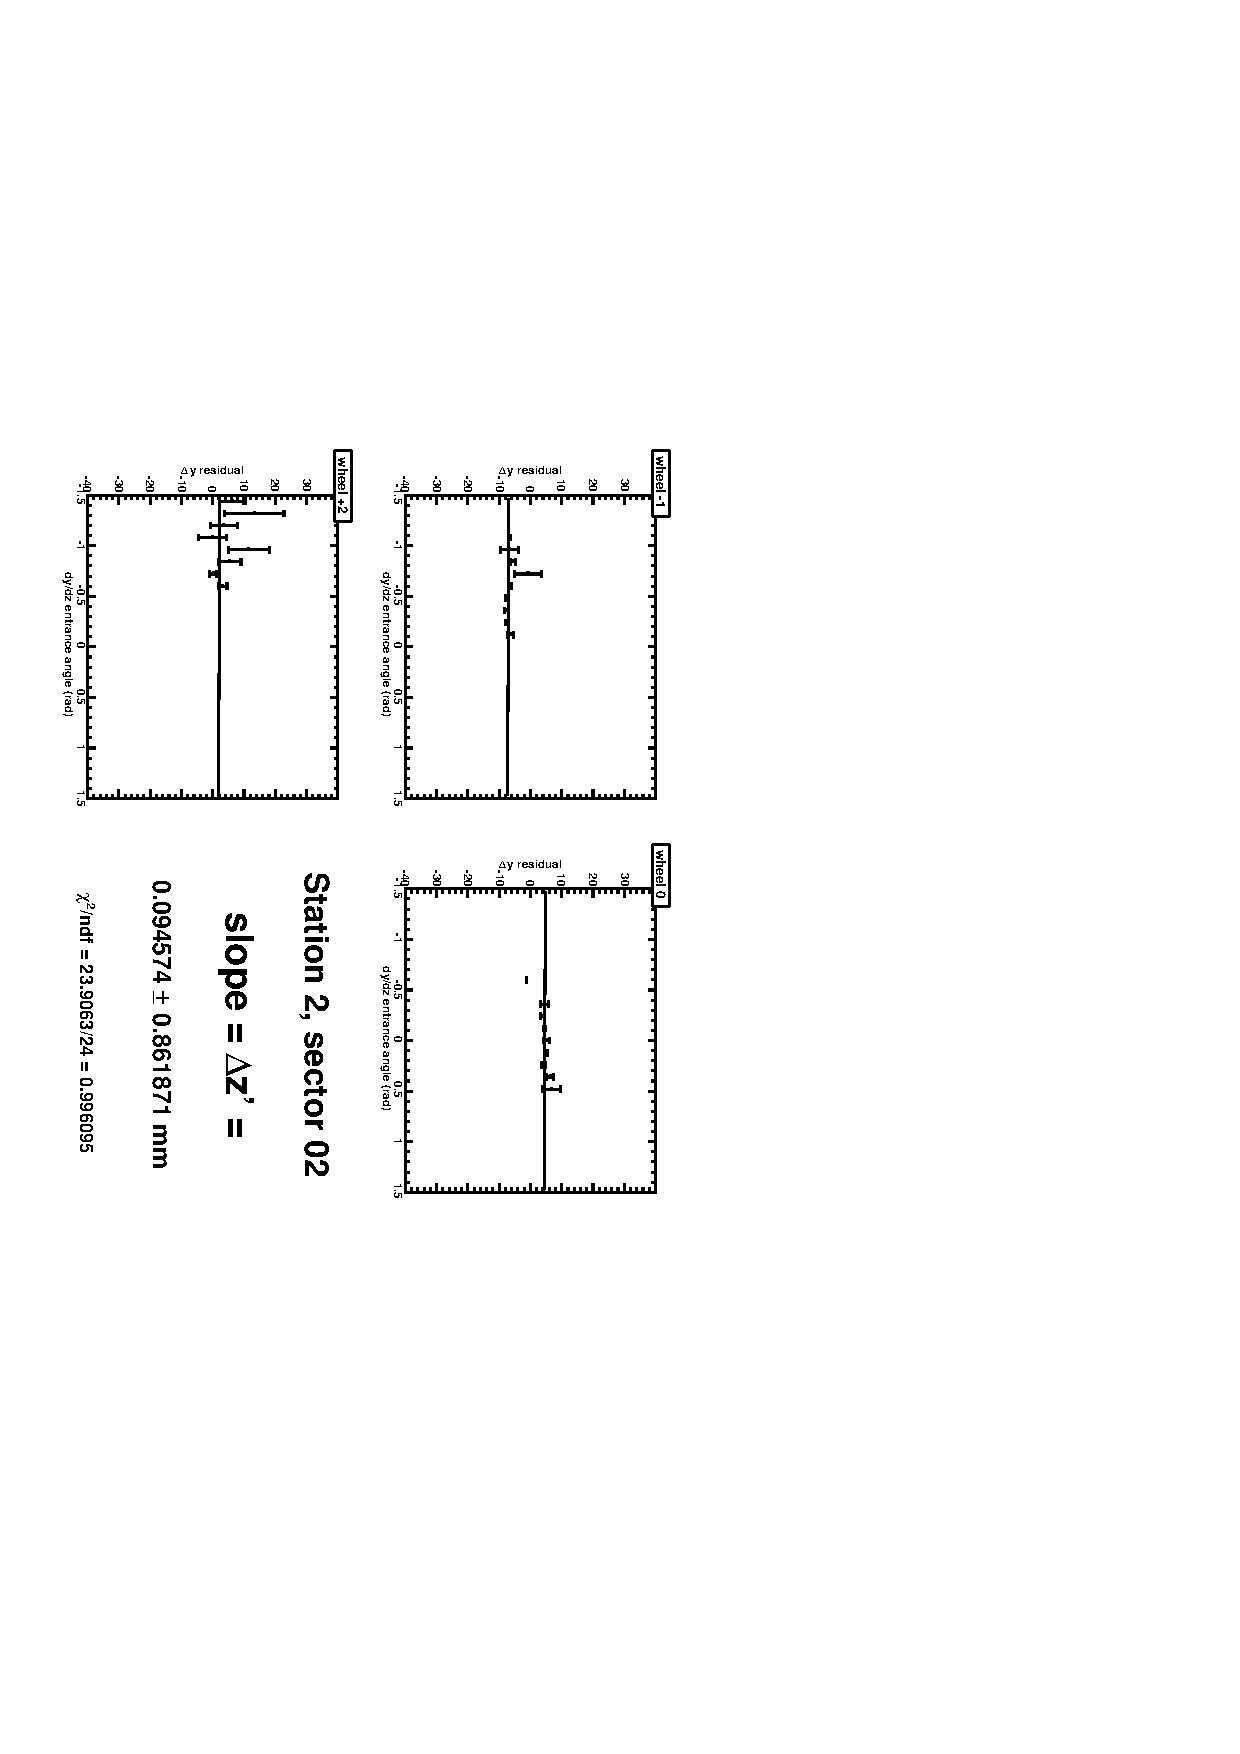
\includegraphics[height=\linewidth, angle=90]{zfits_after/zfit_2_02.pdf}
\column{0.3\linewidth}
\begin{itemize}
\item Top: before \\ Bottom: after
\item Five panels are wheels in the same SemiSuperSector (some are missing)
\item Fit requires all to have the same slope ($\delta_z$), but allows different offsets ($\delta_y$)
\end{itemize}
\end{columns}
\end{frame}

\begin{frame}
\frametitle{Station 2, sector 3}
\begin{columns}
\column{0.7\linewidth}
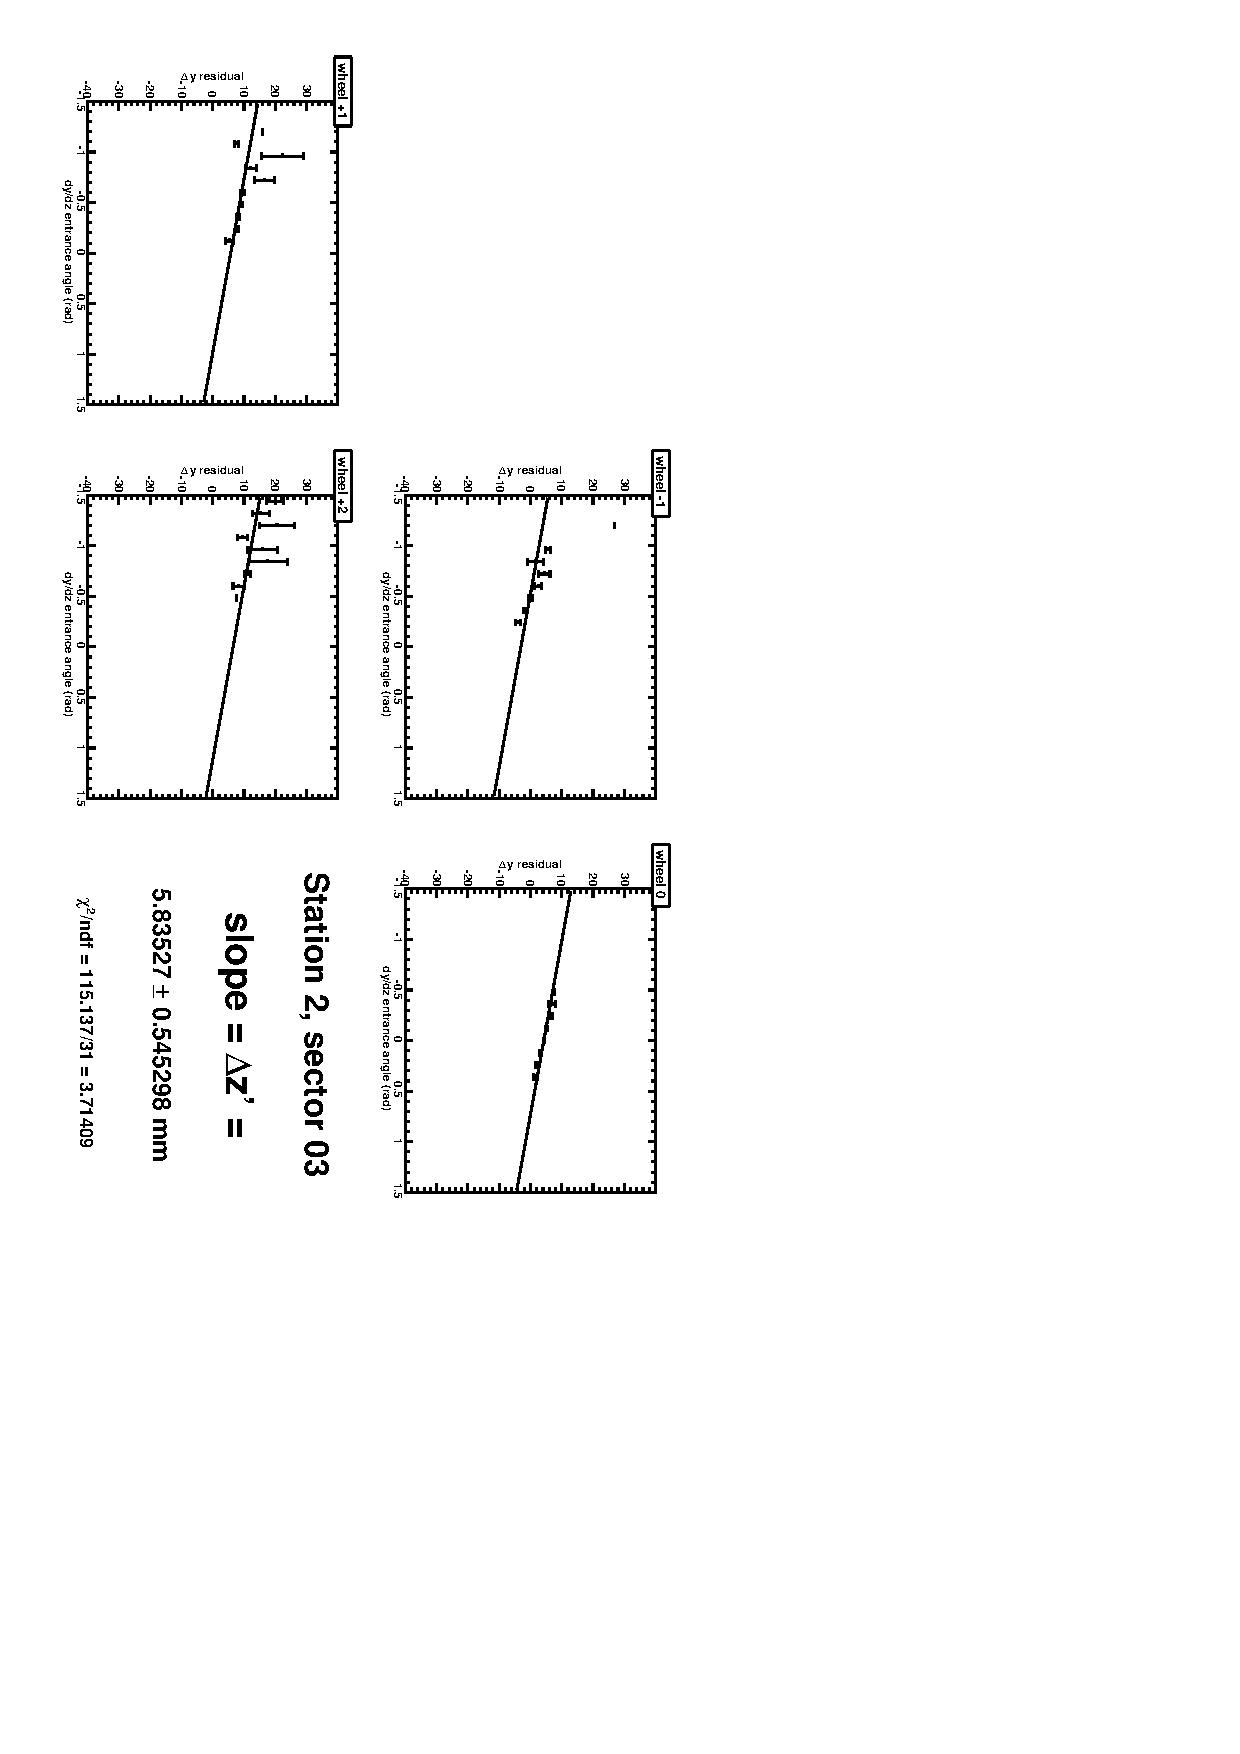
\includegraphics[height=\linewidth, angle=90]{zfits/zfit_2_03.pdf}

\vfill
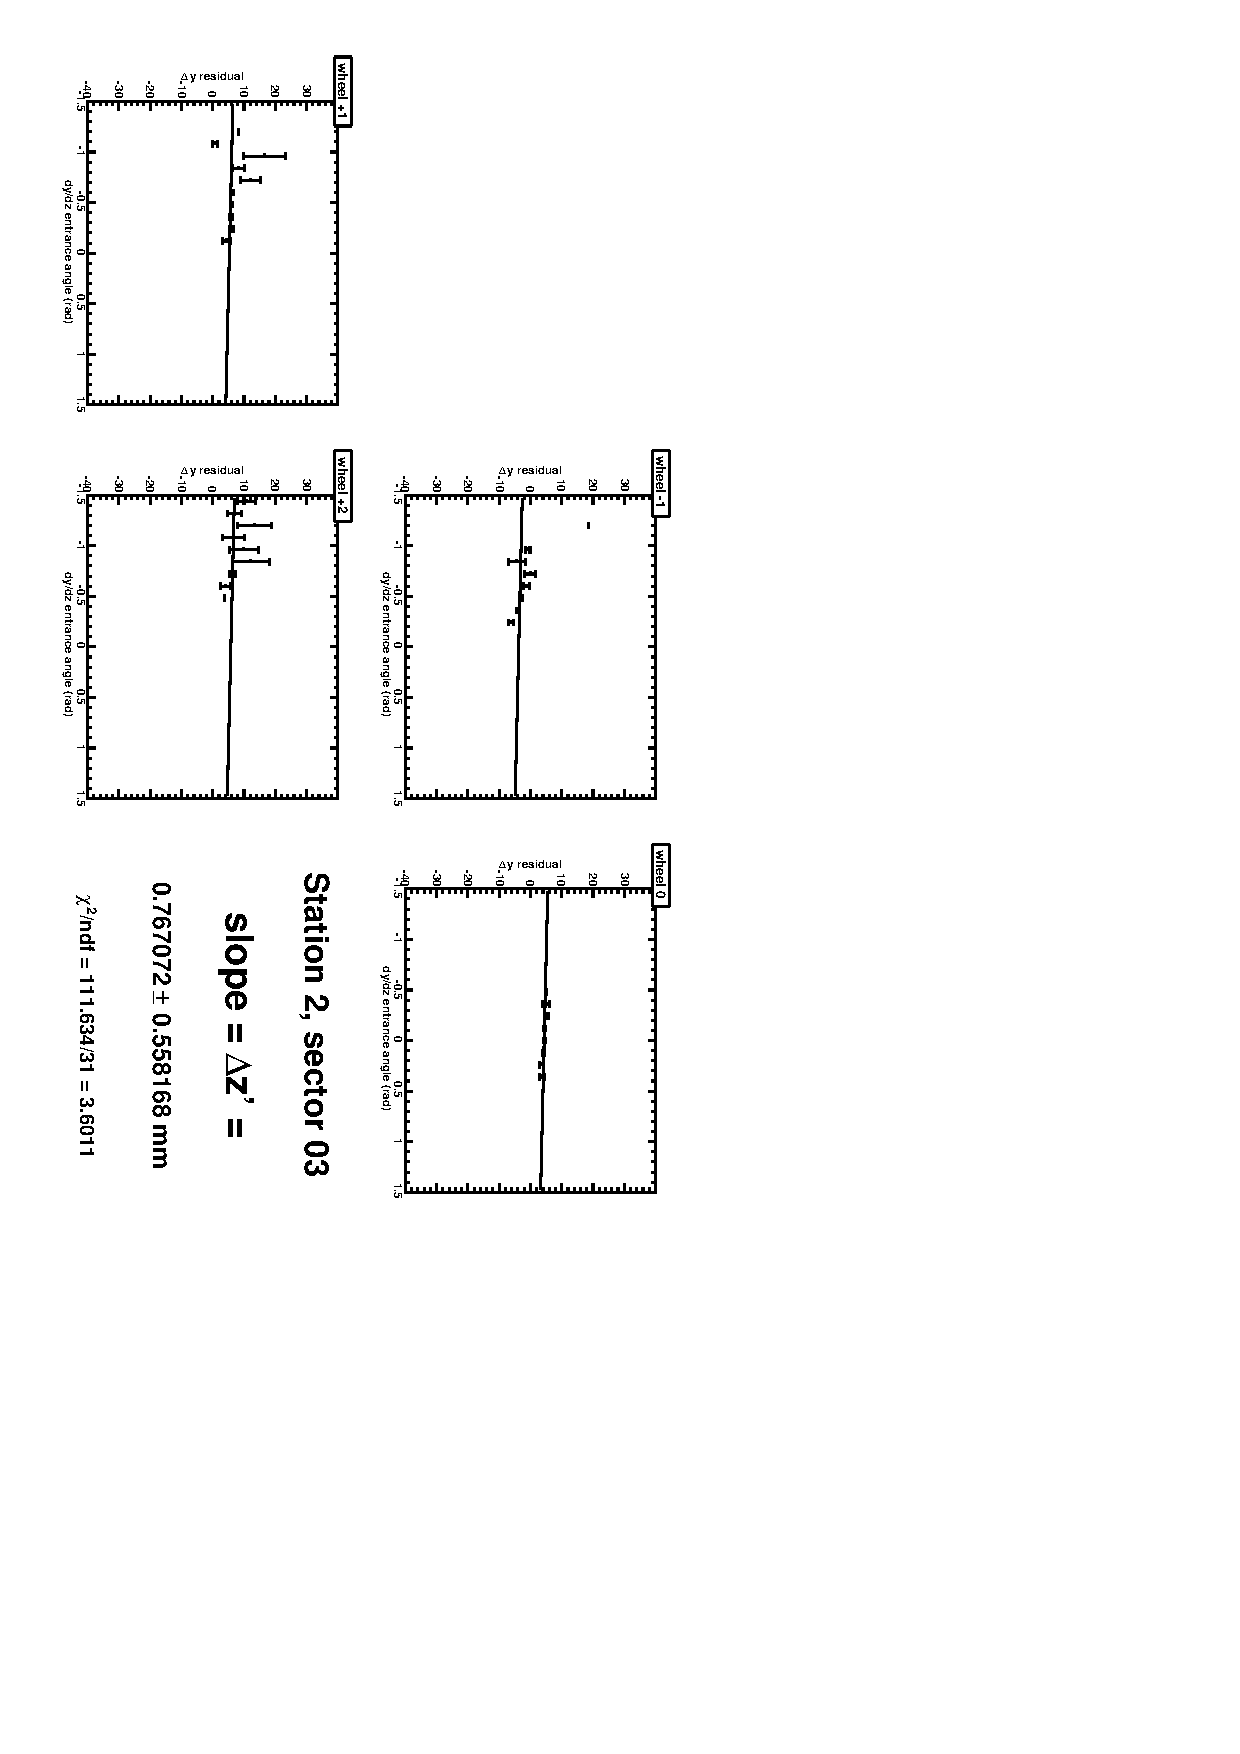
\includegraphics[height=\linewidth, angle=90]{zfits_after/zfit_2_03.pdf}
\column{0.3\linewidth}
\begin{itemize}
\item Top: before \\ Bottom: after
\item Five panels are wheels in the same SemiSuperSector (some are missing)
\item Fit requires all to have the same slope ($\delta_z$), but allows different offsets ($\delta_y$)
\end{itemize}
\end{columns}
\end{frame}

\begin{frame}
\frametitle{Station 2, sector 4}
\begin{columns}
\column{0.7\linewidth}
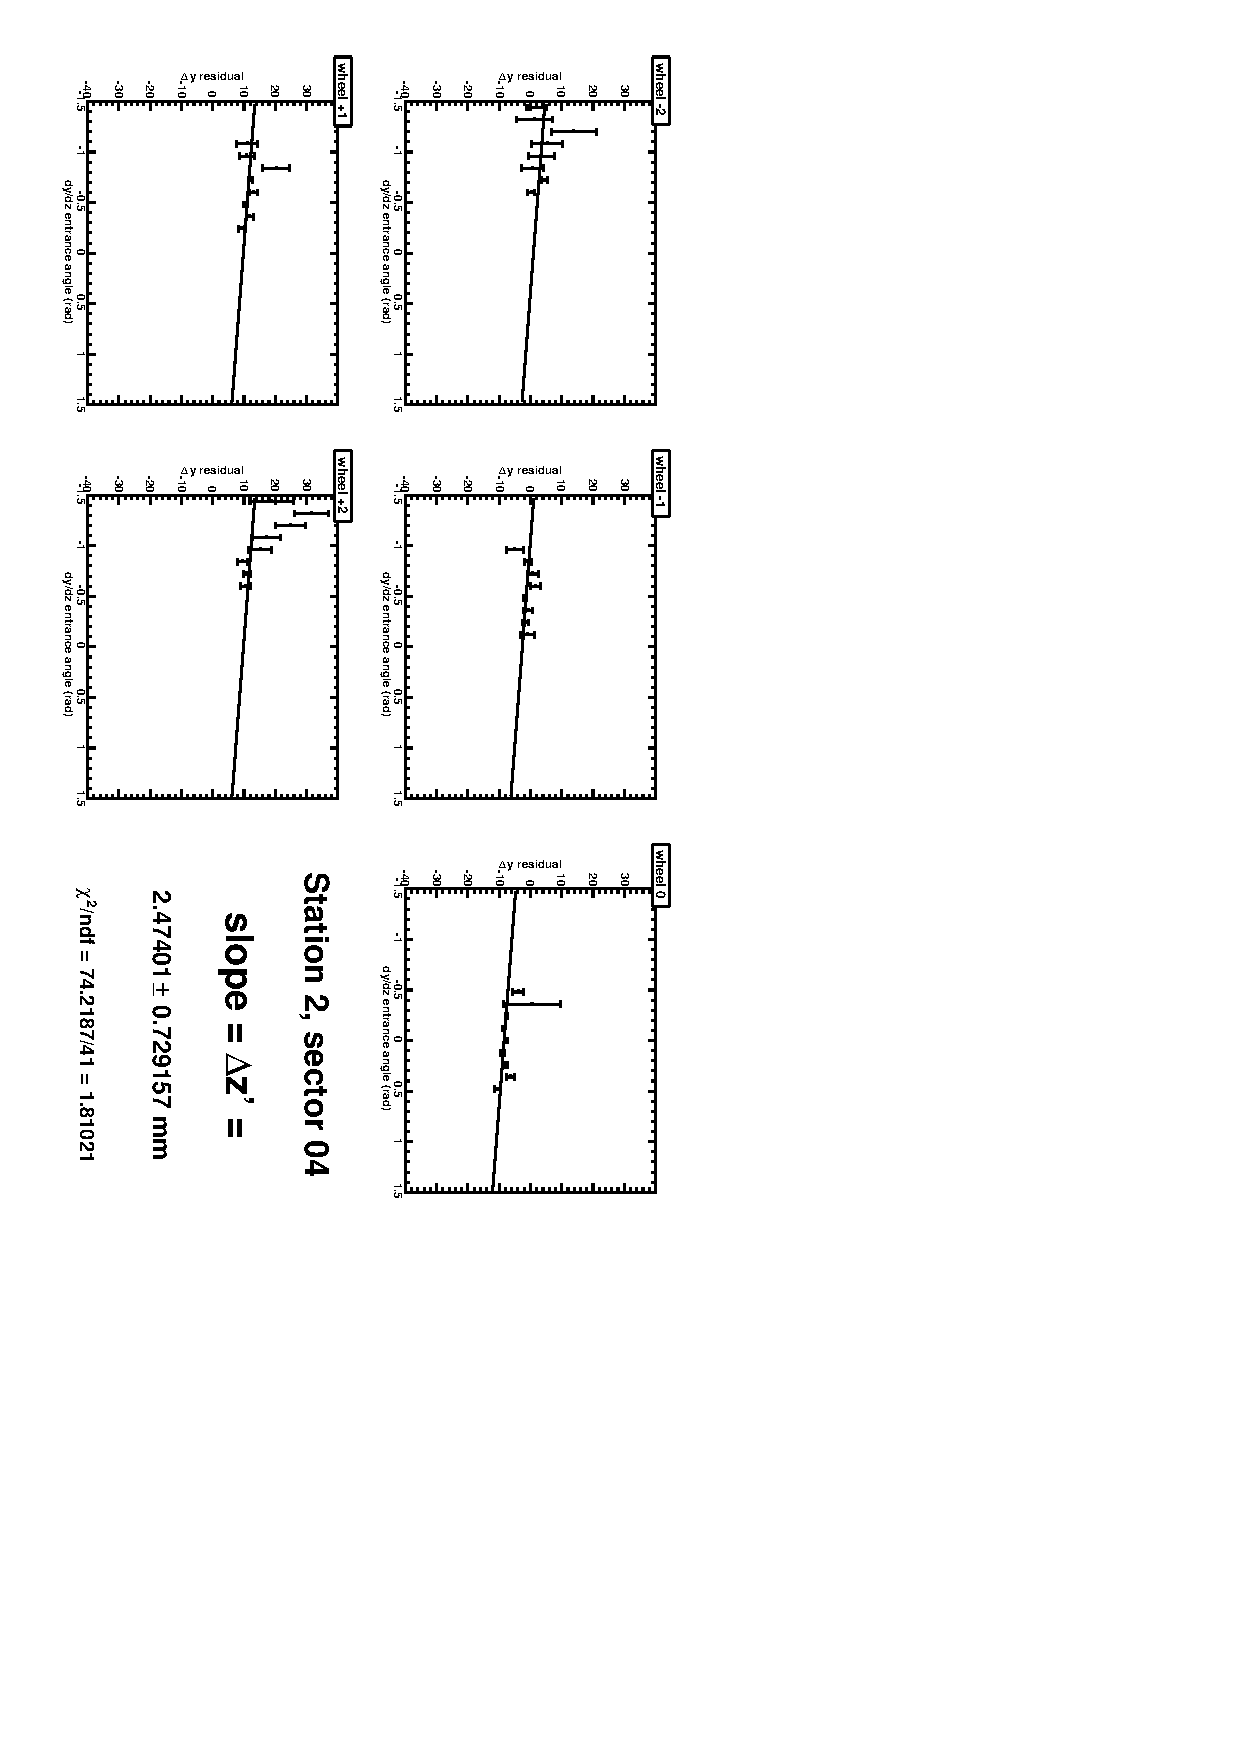
\includegraphics[height=\linewidth, angle=90]{zfits/zfit_2_04.pdf}

\vfill
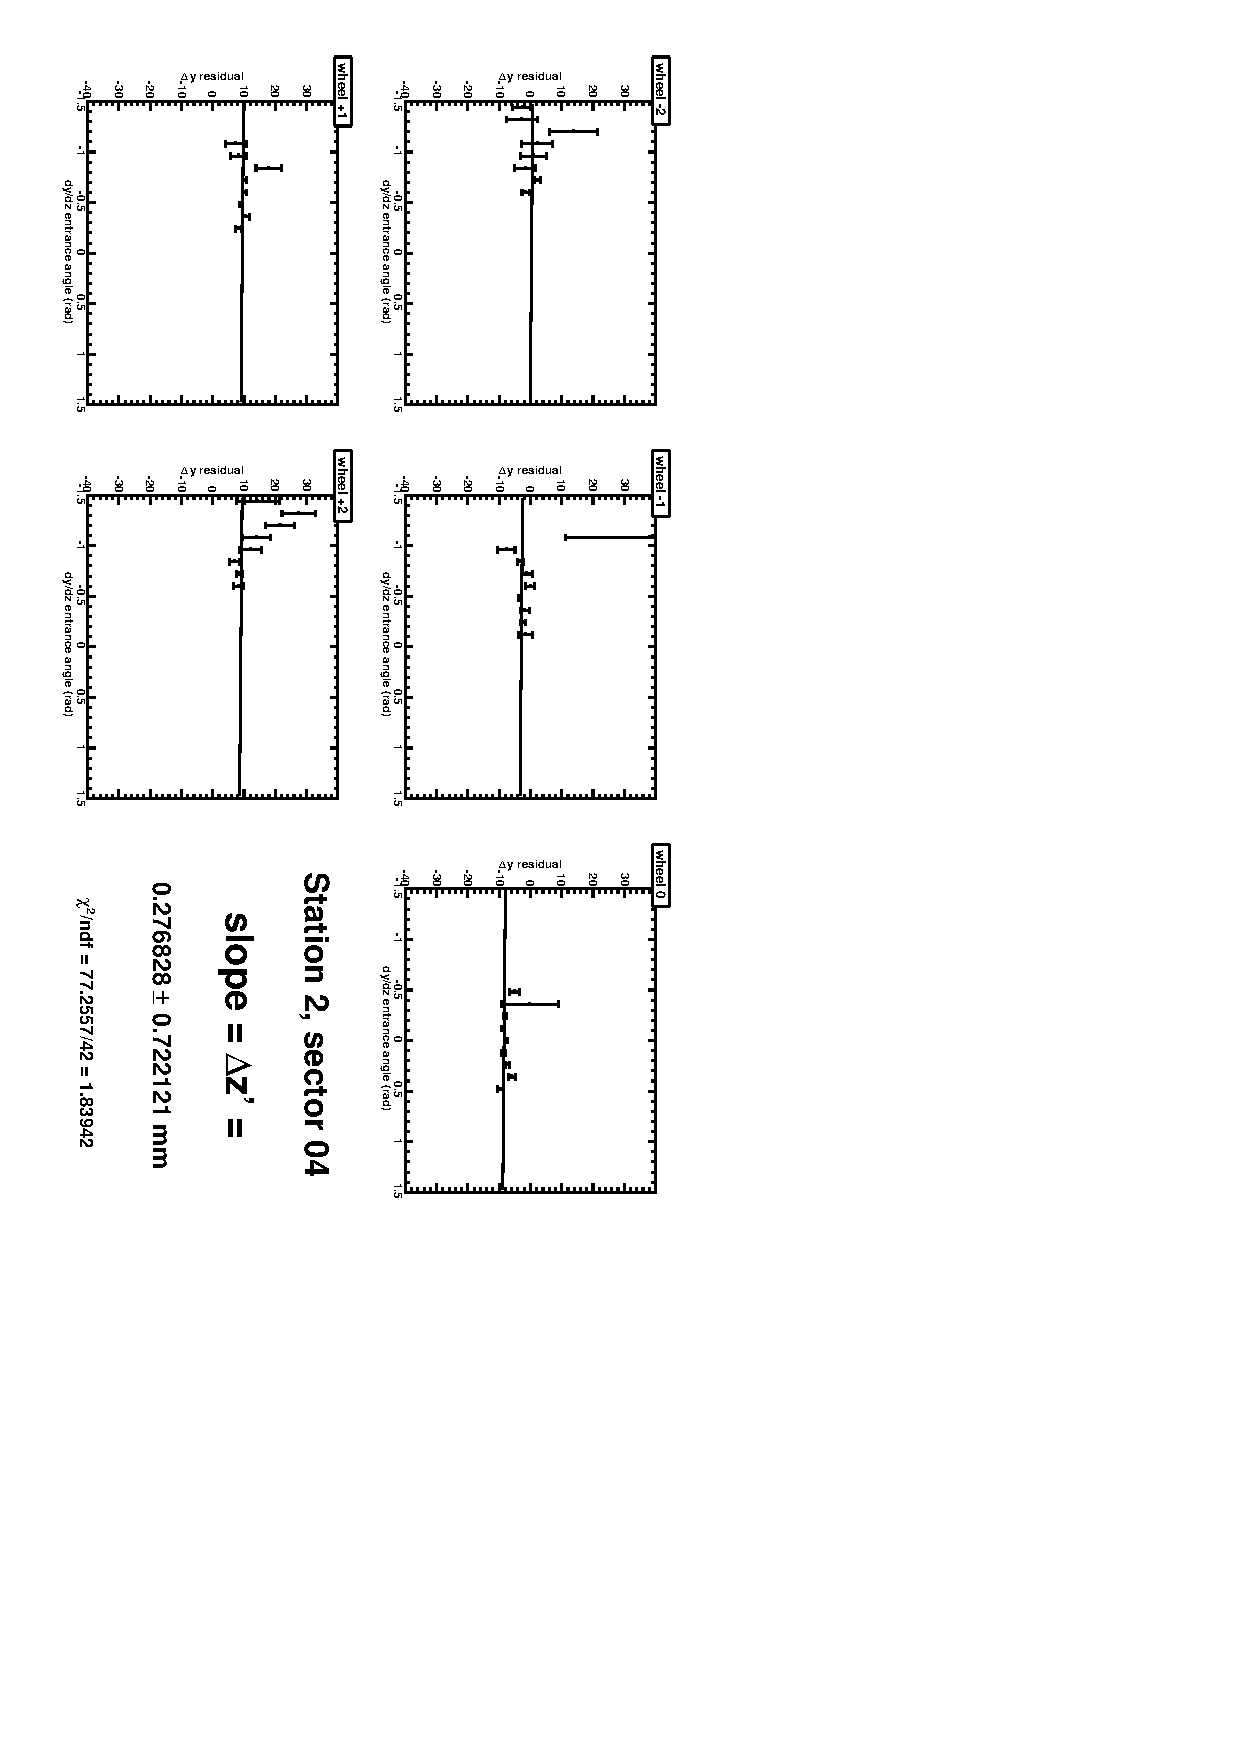
\includegraphics[height=\linewidth, angle=90]{zfits_after/zfit_2_04.pdf}
\column{0.3\linewidth}
\begin{itemize}
\item Top: before \\ Bottom: after
\item Five panels are wheels in the same SemiSuperSector (some are missing)
\item Fit requires all to have the same slope ($\delta_z$), but allows different offsets ($\delta_y$)
\end{itemize}
\end{columns}
\end{frame}

\begin{frame}
\frametitle{Station 2, sector 5}
\begin{columns}
\column{0.7\linewidth}
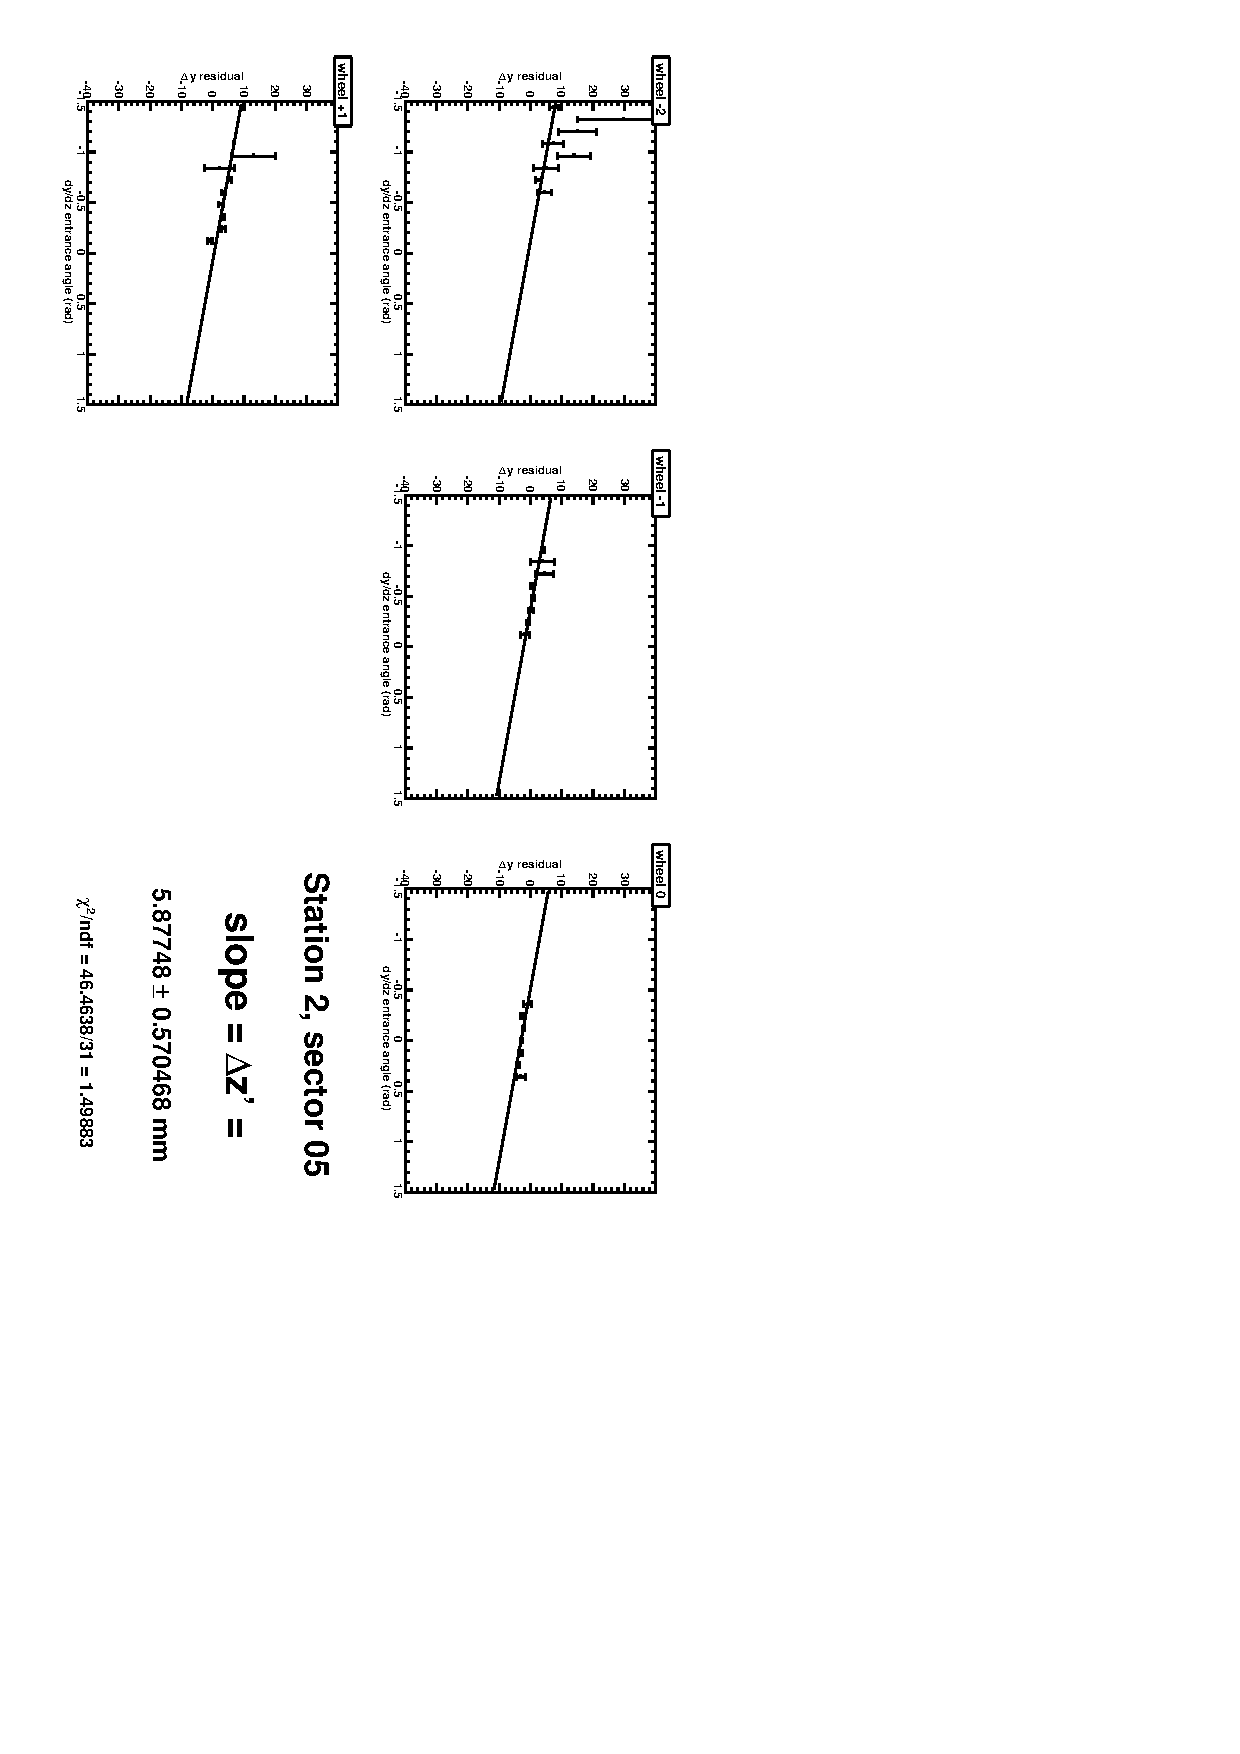
\includegraphics[height=\linewidth, angle=90]{zfits/zfit_2_05.pdf}

\vfill
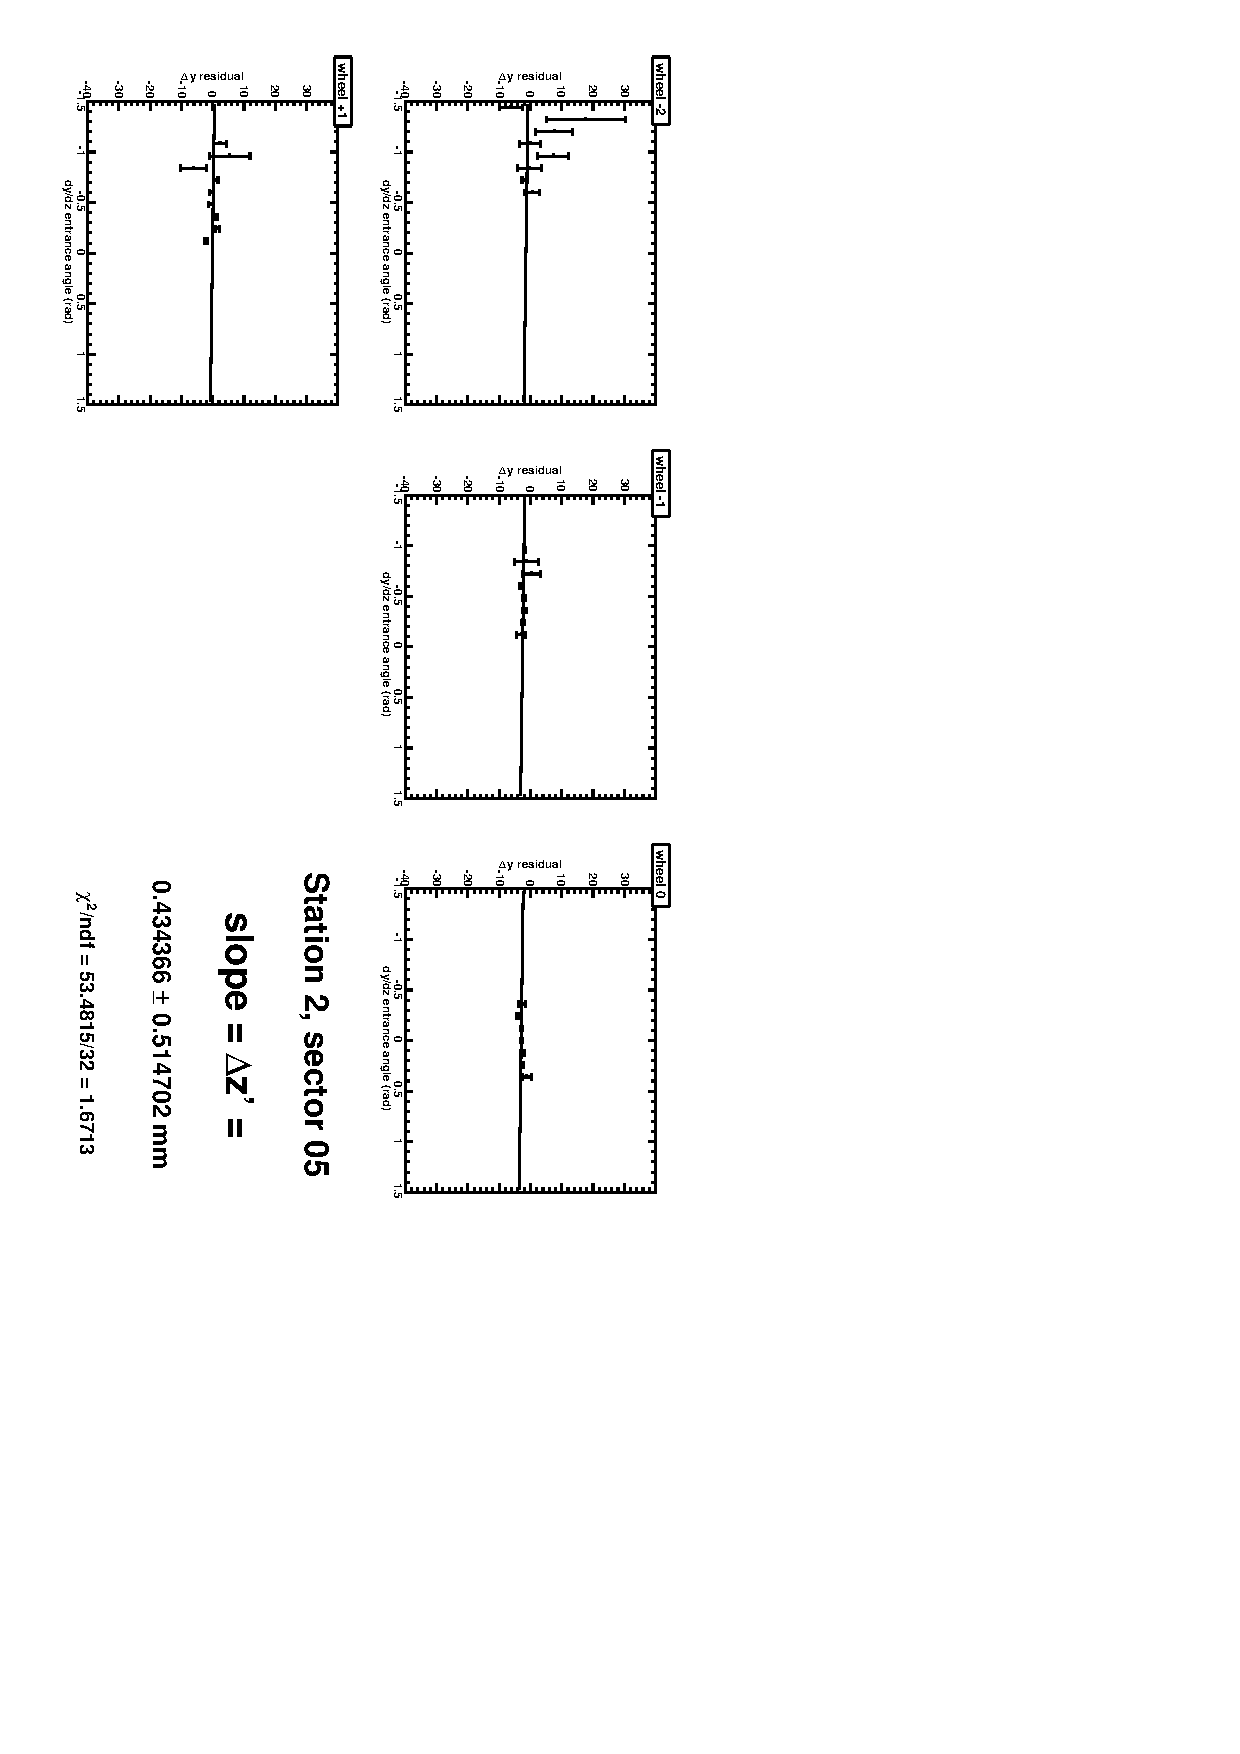
\includegraphics[height=\linewidth, angle=90]{zfits_after/zfit_2_05.pdf}
\column{0.3\linewidth}
\begin{itemize}
\item Top: before \\ Bottom: after
\item Five panels are wheels in the same SemiSuperSector (some are missing)
\item Fit requires all to have the same slope ($\delta_z$), but allows different offsets ($\delta_y$)
\end{itemize}
\end{columns}
\end{frame}

\begin{frame}
\frametitle{Station 2, sector 6}
\begin{columns}
\column{0.7\linewidth}
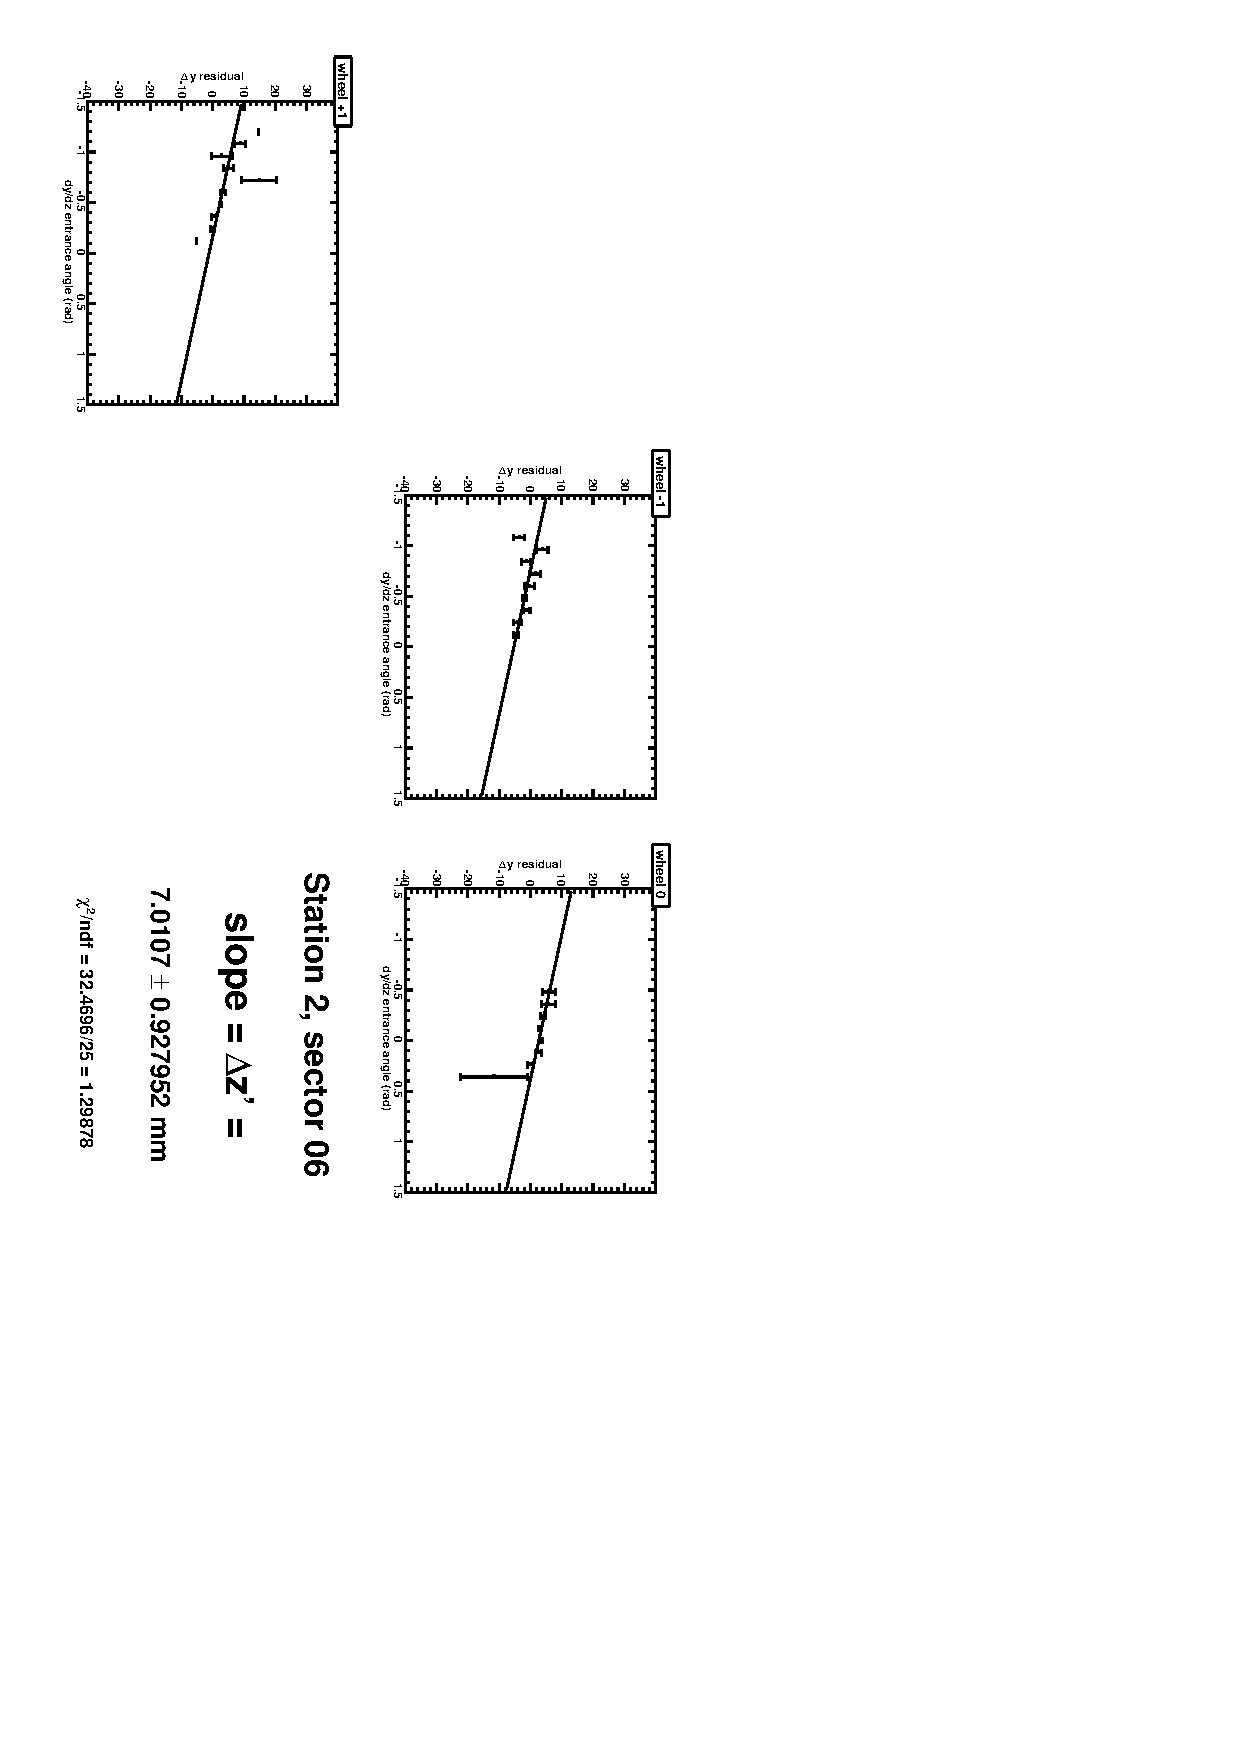
\includegraphics[height=\linewidth, angle=90]{zfits/zfit_2_06.pdf}

\vfill
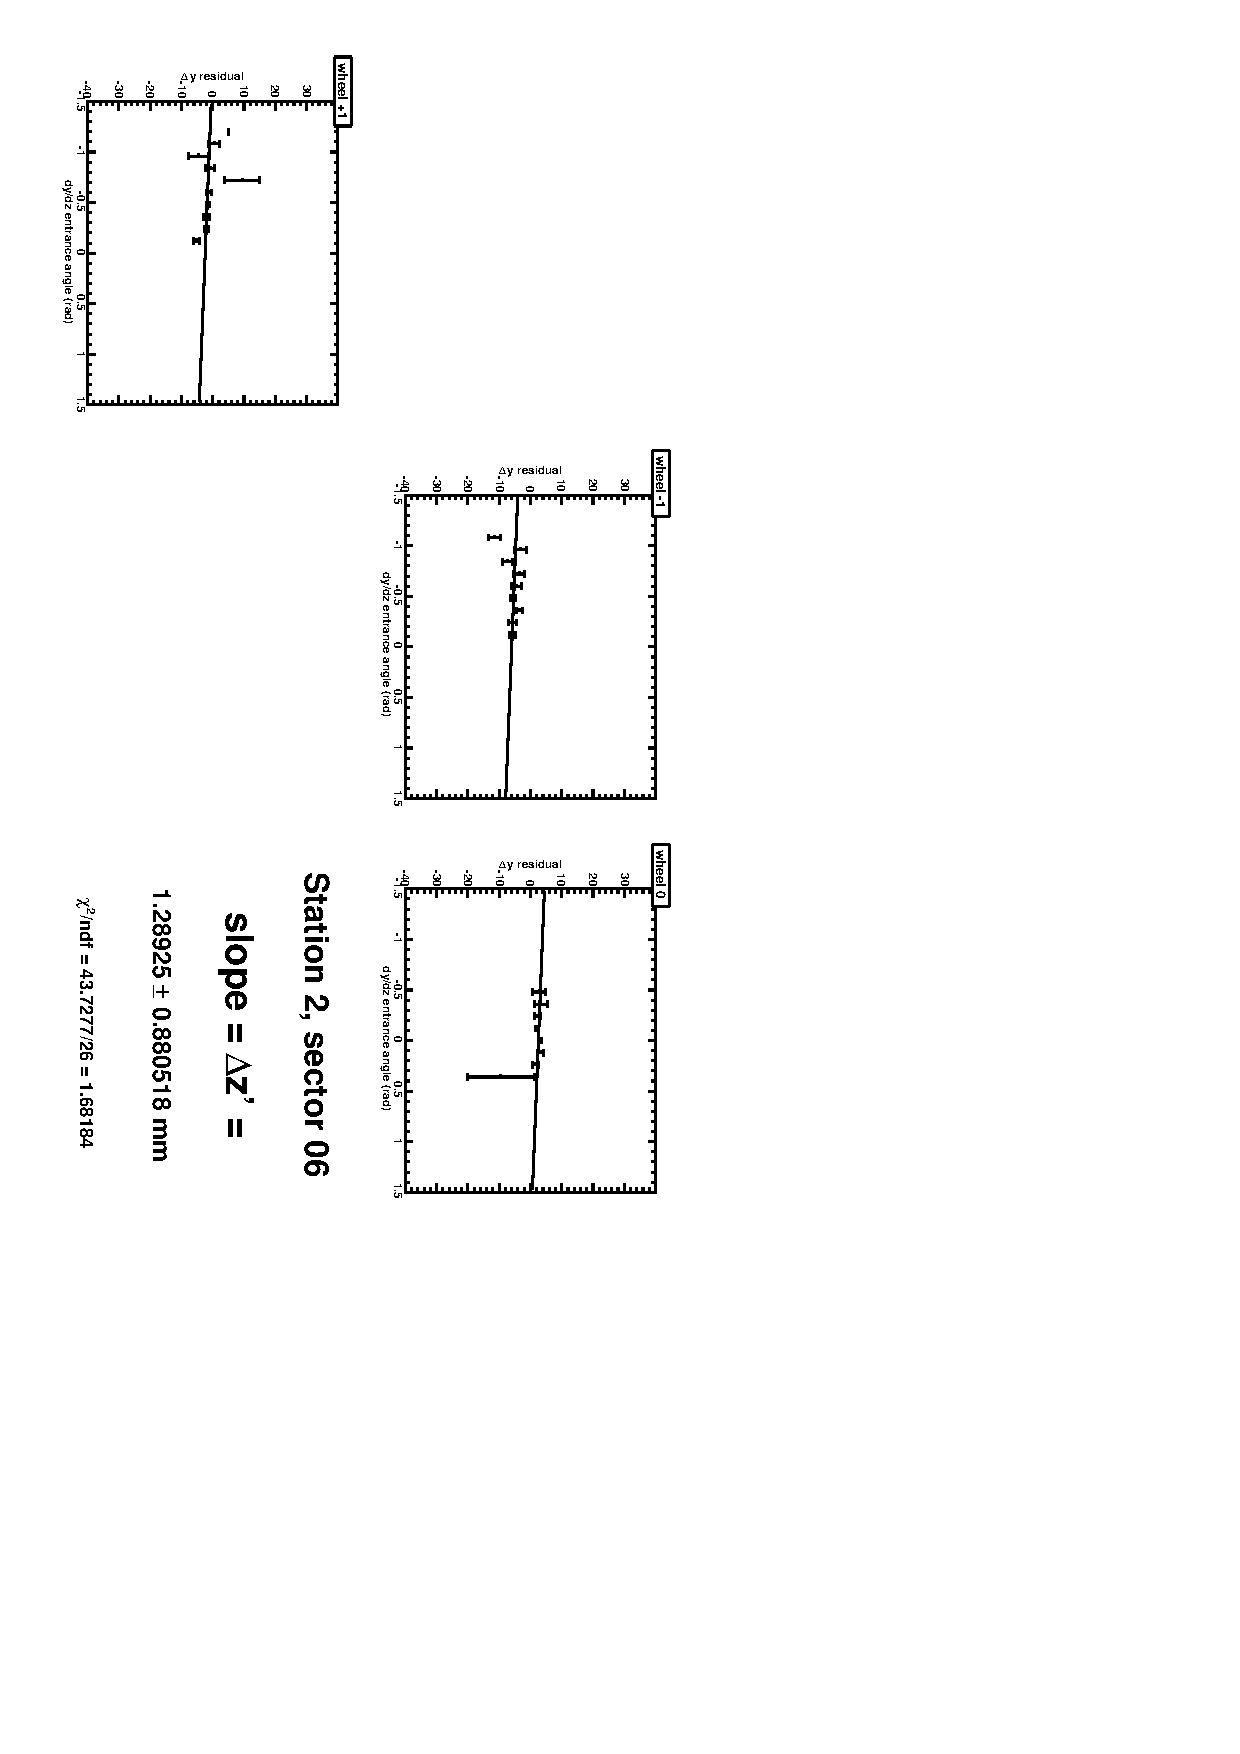
\includegraphics[height=\linewidth, angle=90]{zfits_after/zfit_2_06.pdf}
\column{0.3\linewidth}
\begin{itemize}
\item Top: before \\ Bottom: after
\item Five panels are wheels in the same SemiSuperSector (some are missing)
\item Fit requires all to have the same slope ($\delta_z$), but allows different offsets ($\delta_y$)
\end{itemize}
\end{columns}
\end{frame}

\begin{frame}
\frametitle{Station 2, sector 8}
\begin{columns}
\column{0.7\linewidth}
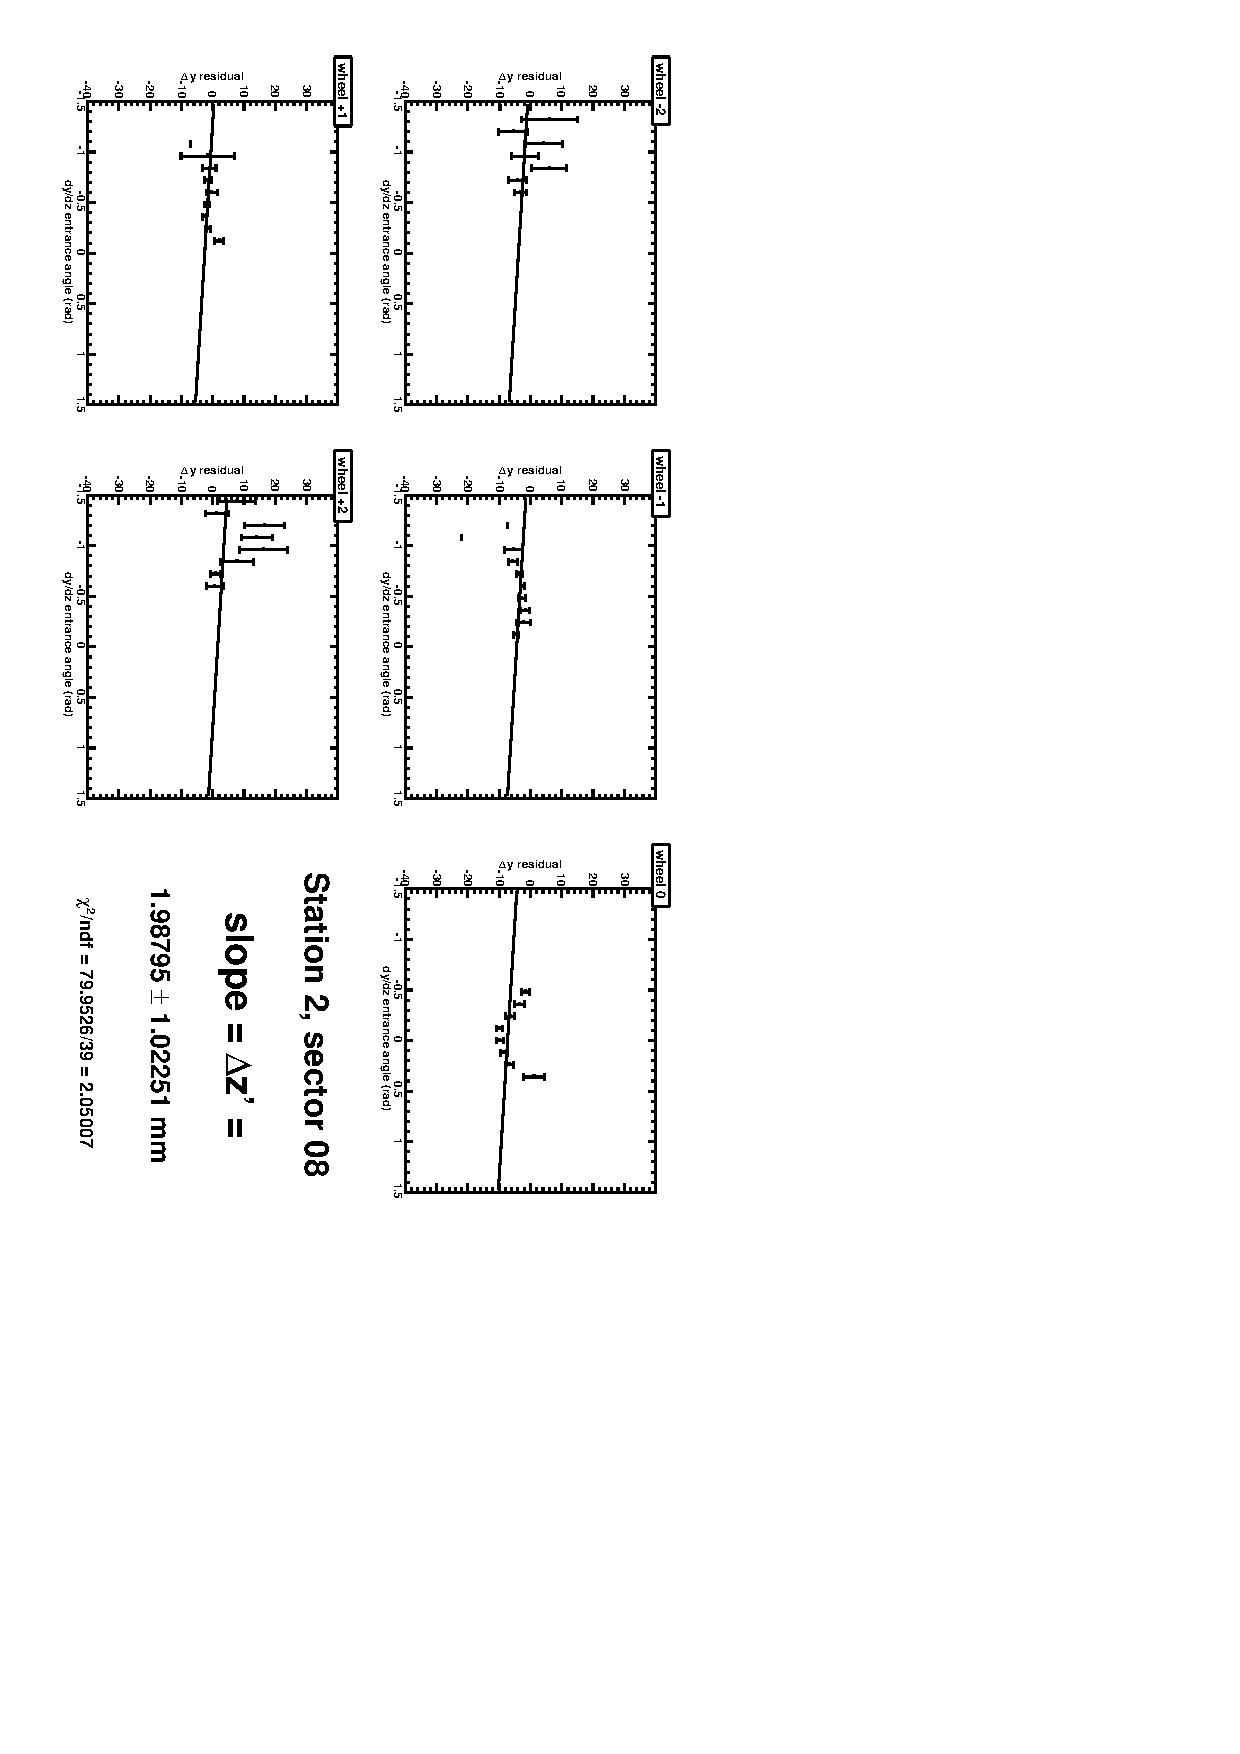
\includegraphics[height=\linewidth, angle=90]{zfits/zfit_2_08.pdf}

\vfill
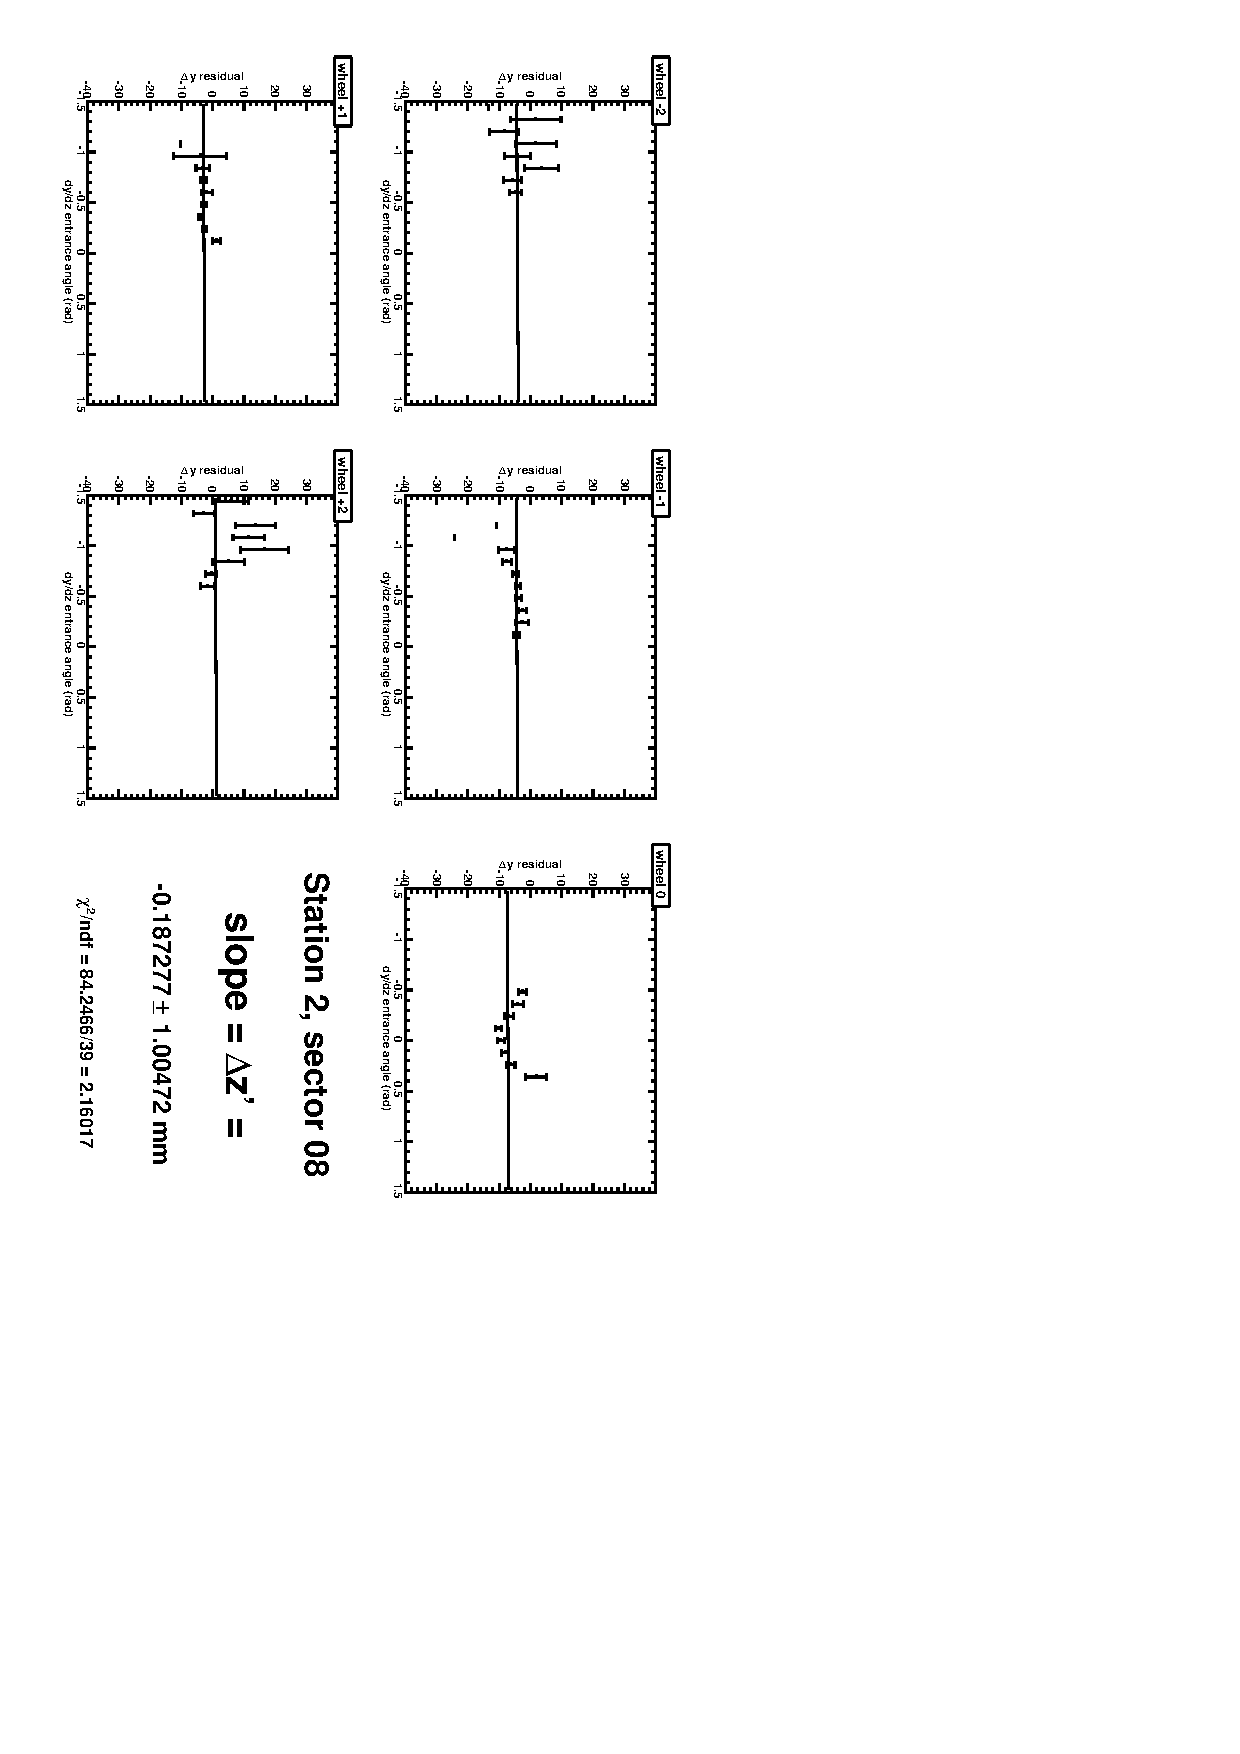
\includegraphics[height=\linewidth, angle=90]{zfits_after/zfit_2_08.pdf}
\column{0.3\linewidth}
\begin{itemize}
\item Top: before \\ Bottom: after
\item Five panels are wheels in the same SemiSuperSector (some are missing)
\item Fit requires all to have the same slope ($\delta_z$), but allows different offsets ($\delta_y$)
\end{itemize}
\end{columns}
\end{frame}

\begin{frame}
\frametitle{Station 2, sector 9}
\begin{columns}
\column{0.7\linewidth}
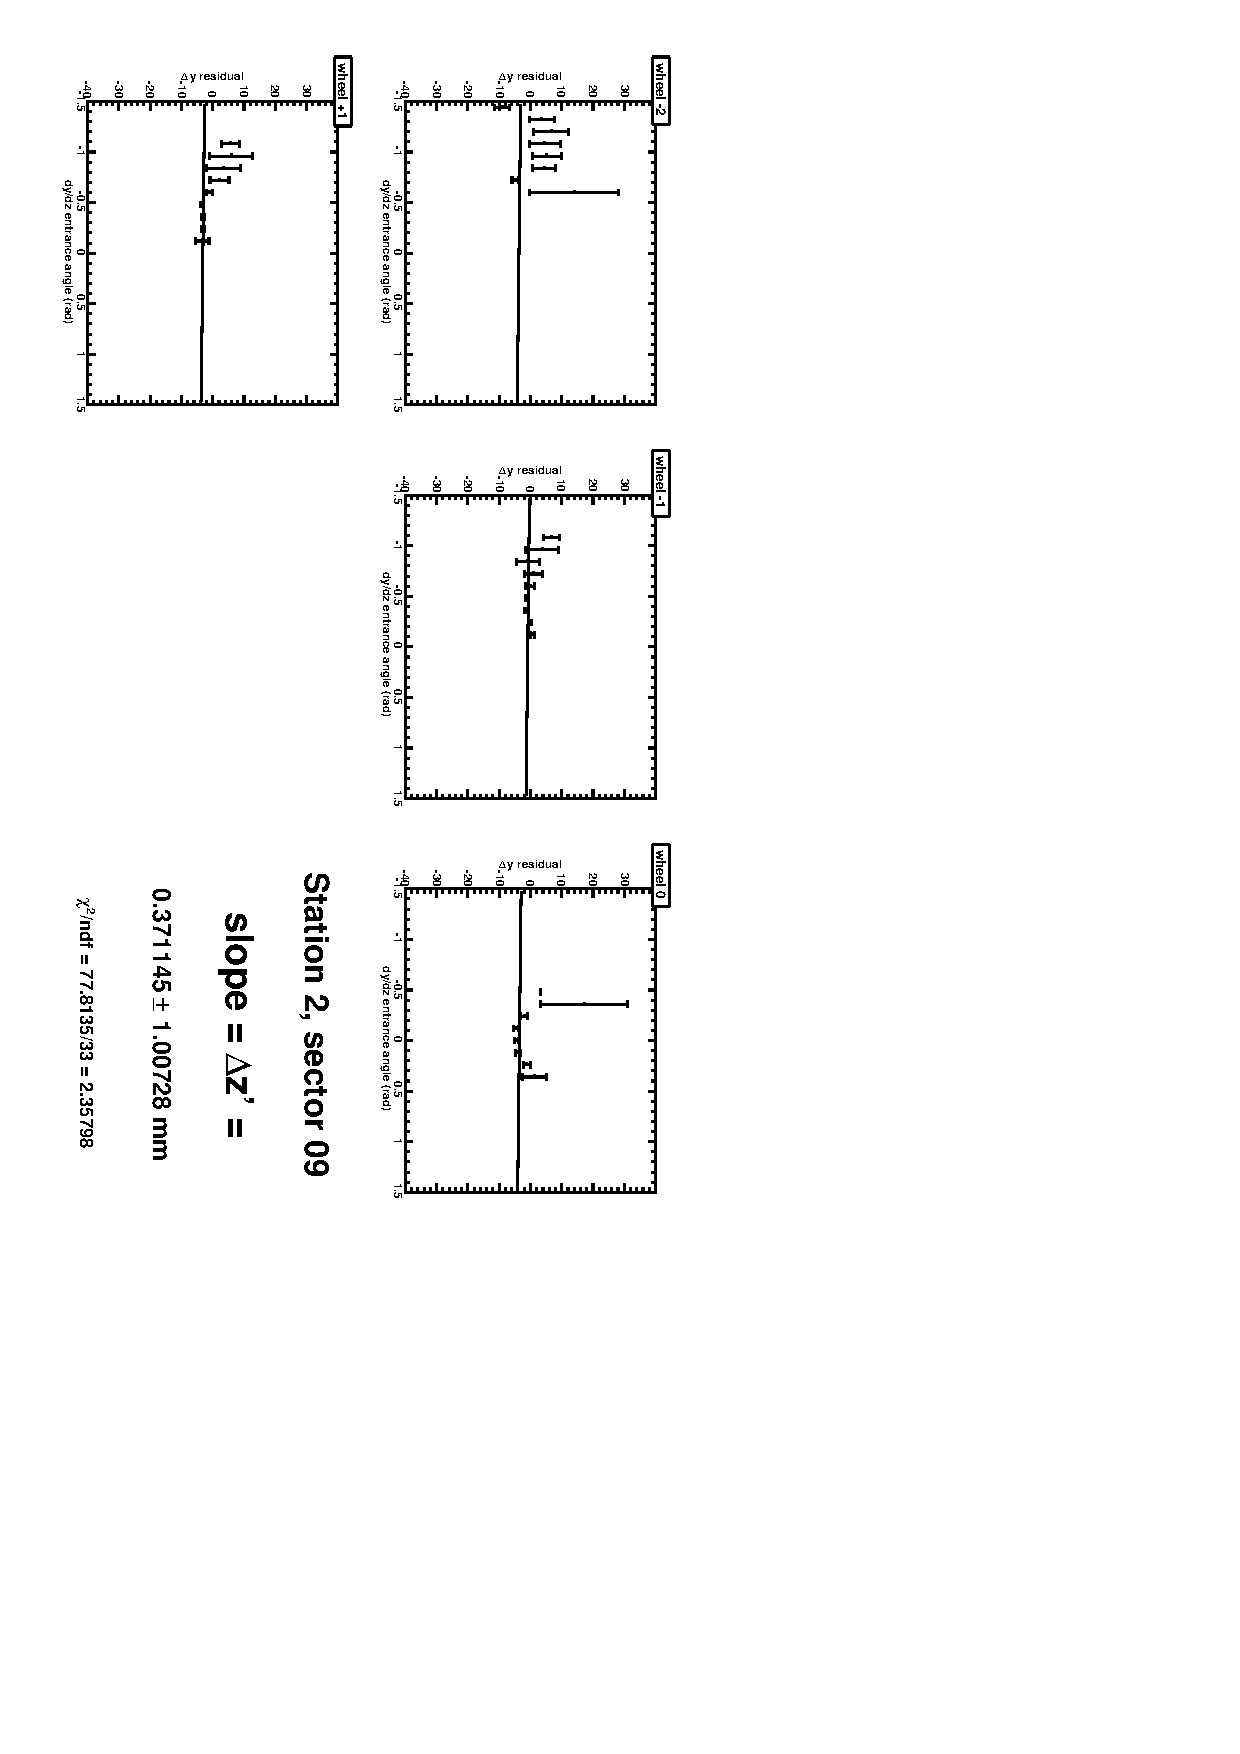
\includegraphics[height=\linewidth, angle=90]{zfits/zfit_2_09.pdf}

\vfill
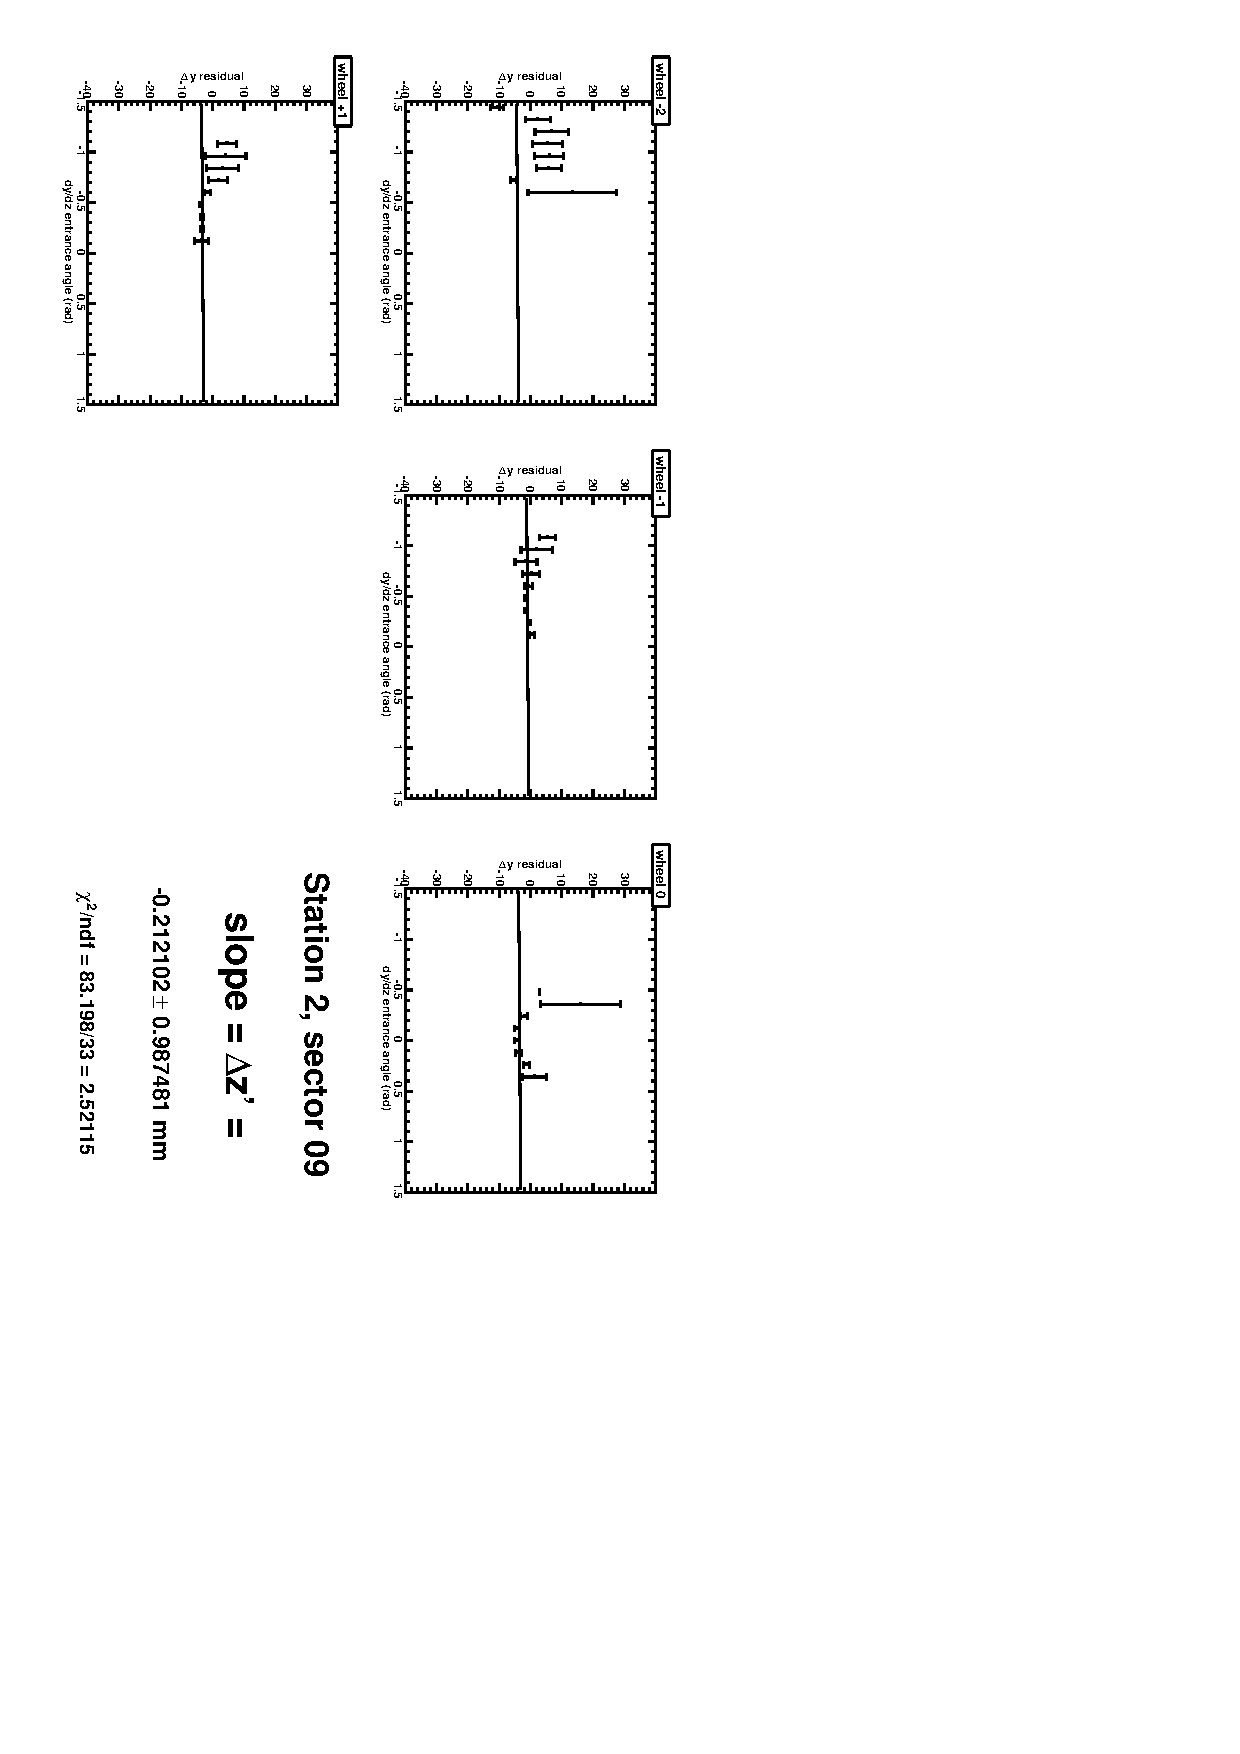
\includegraphics[height=\linewidth, angle=90]{zfits_after/zfit_2_09.pdf}
\column{0.3\linewidth}
\begin{itemize}
\item Top: before \\ Bottom: after
\item Five panels are wheels in the same SemiSuperSector (some are missing)
\item Fit requires all to have the same slope ($\delta_z$), but allows different offsets ($\delta_y$)
\end{itemize}
\end{columns}
\end{frame}

\begin{frame}
\frametitle{Station 2, sector 10}
\begin{columns}
\column{0.7\linewidth}
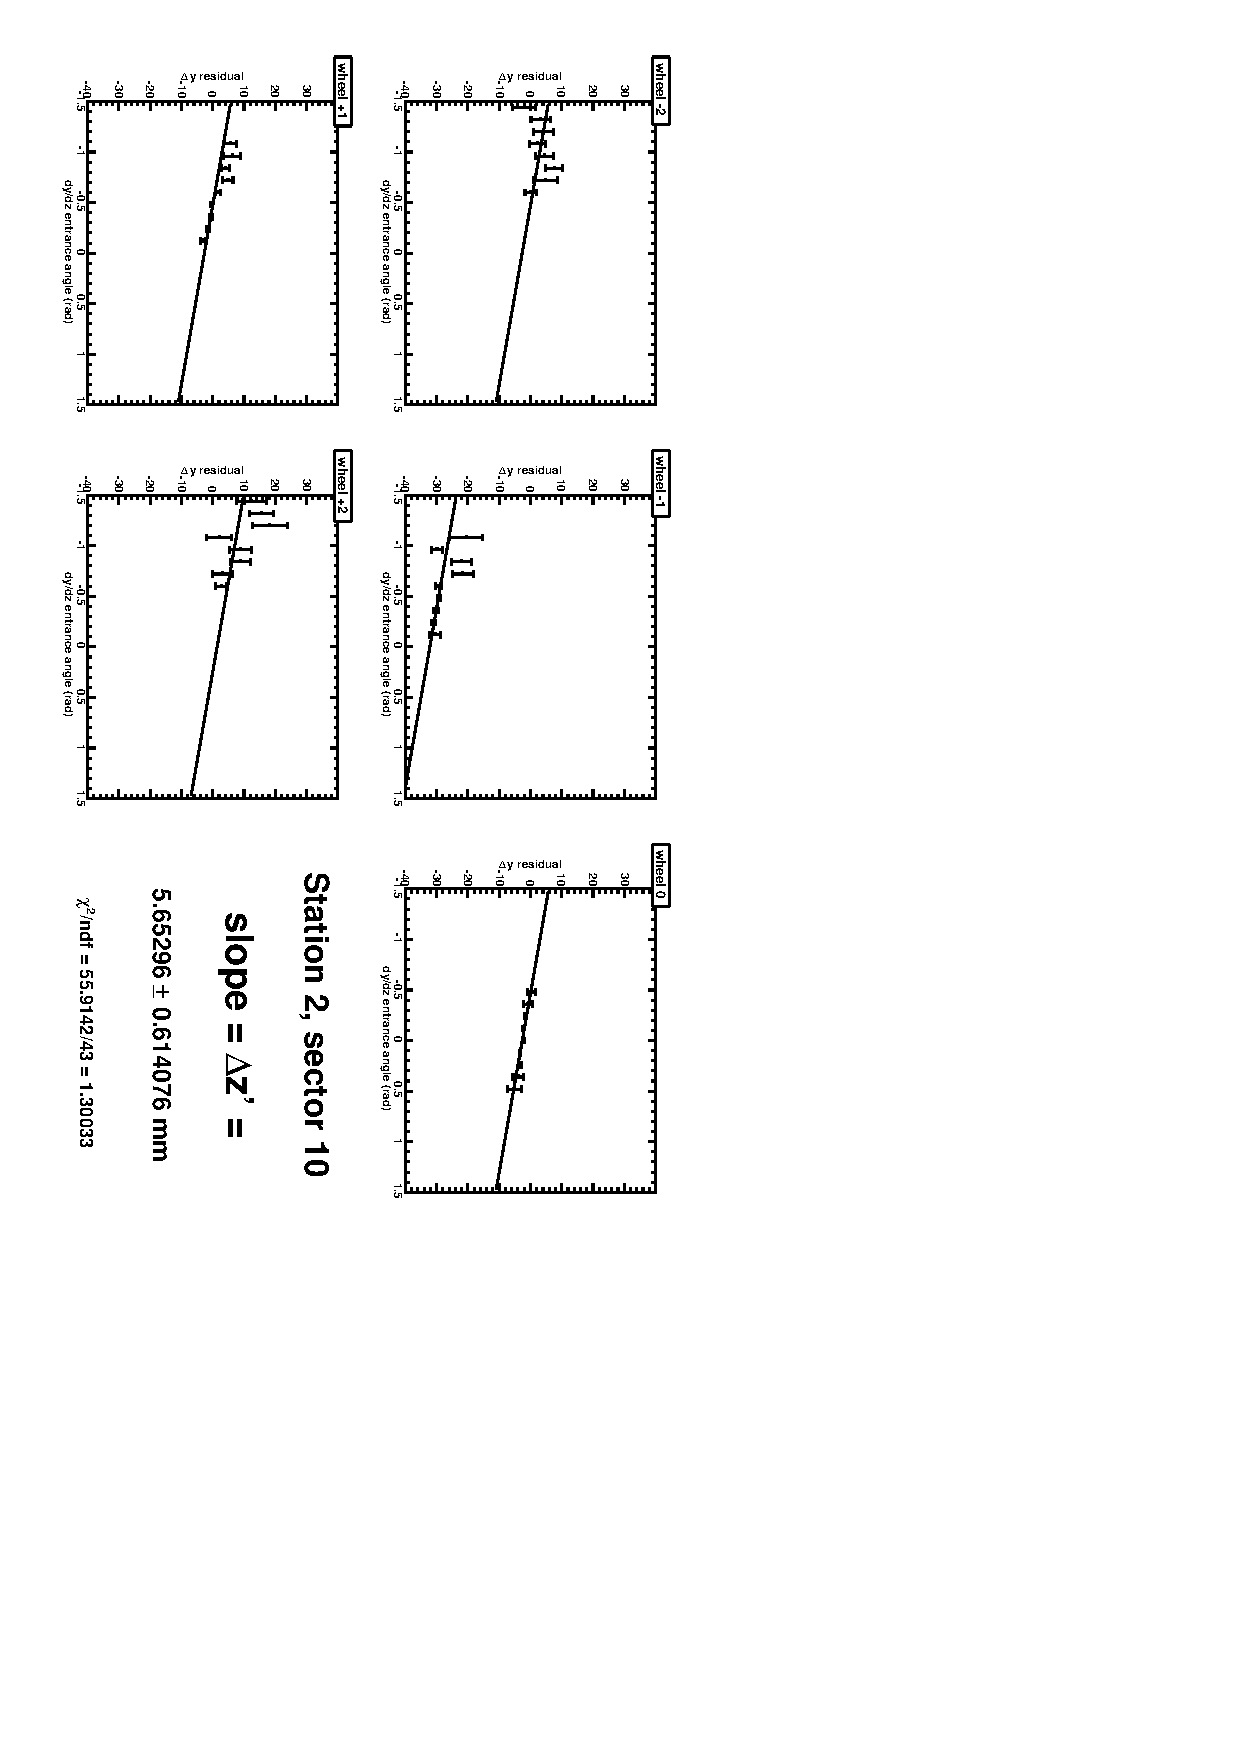
\includegraphics[height=\linewidth, angle=90]{zfits/zfit_2_10.pdf}

\vfill
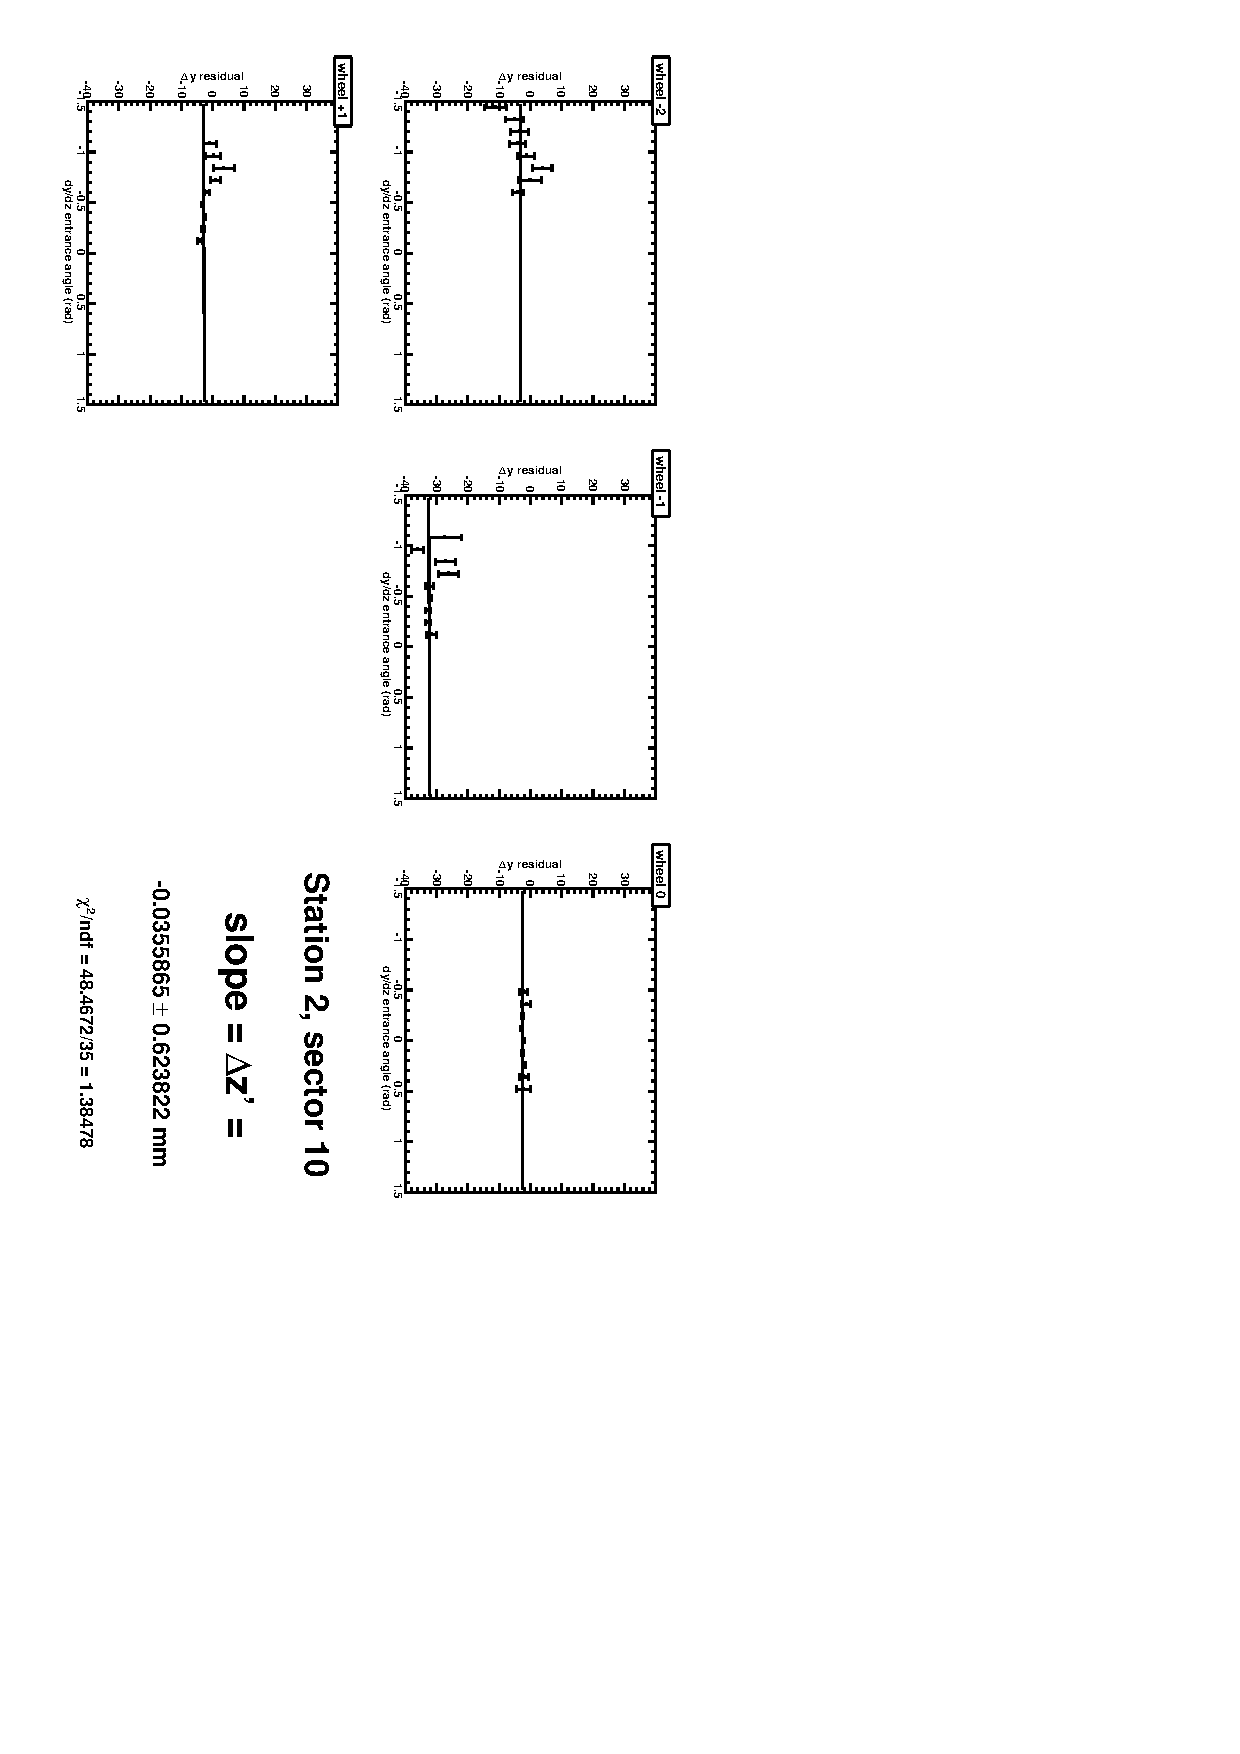
\includegraphics[height=\linewidth, angle=90]{zfits_after/zfit_2_10.pdf}
\column{0.3\linewidth}
\begin{itemize}
\item Top: before \\ Bottom: after
\item Five panels are wheels in the same SemiSuperSector (some are missing)
\item Fit requires all to have the same slope ($\delta_z$), but allows different offsets ($\delta_y$)
\end{itemize}
\end{columns}
\end{frame}

\begin{frame}
\frametitle{Station 2, sector 11}
\begin{columns}
\column{0.7\linewidth}
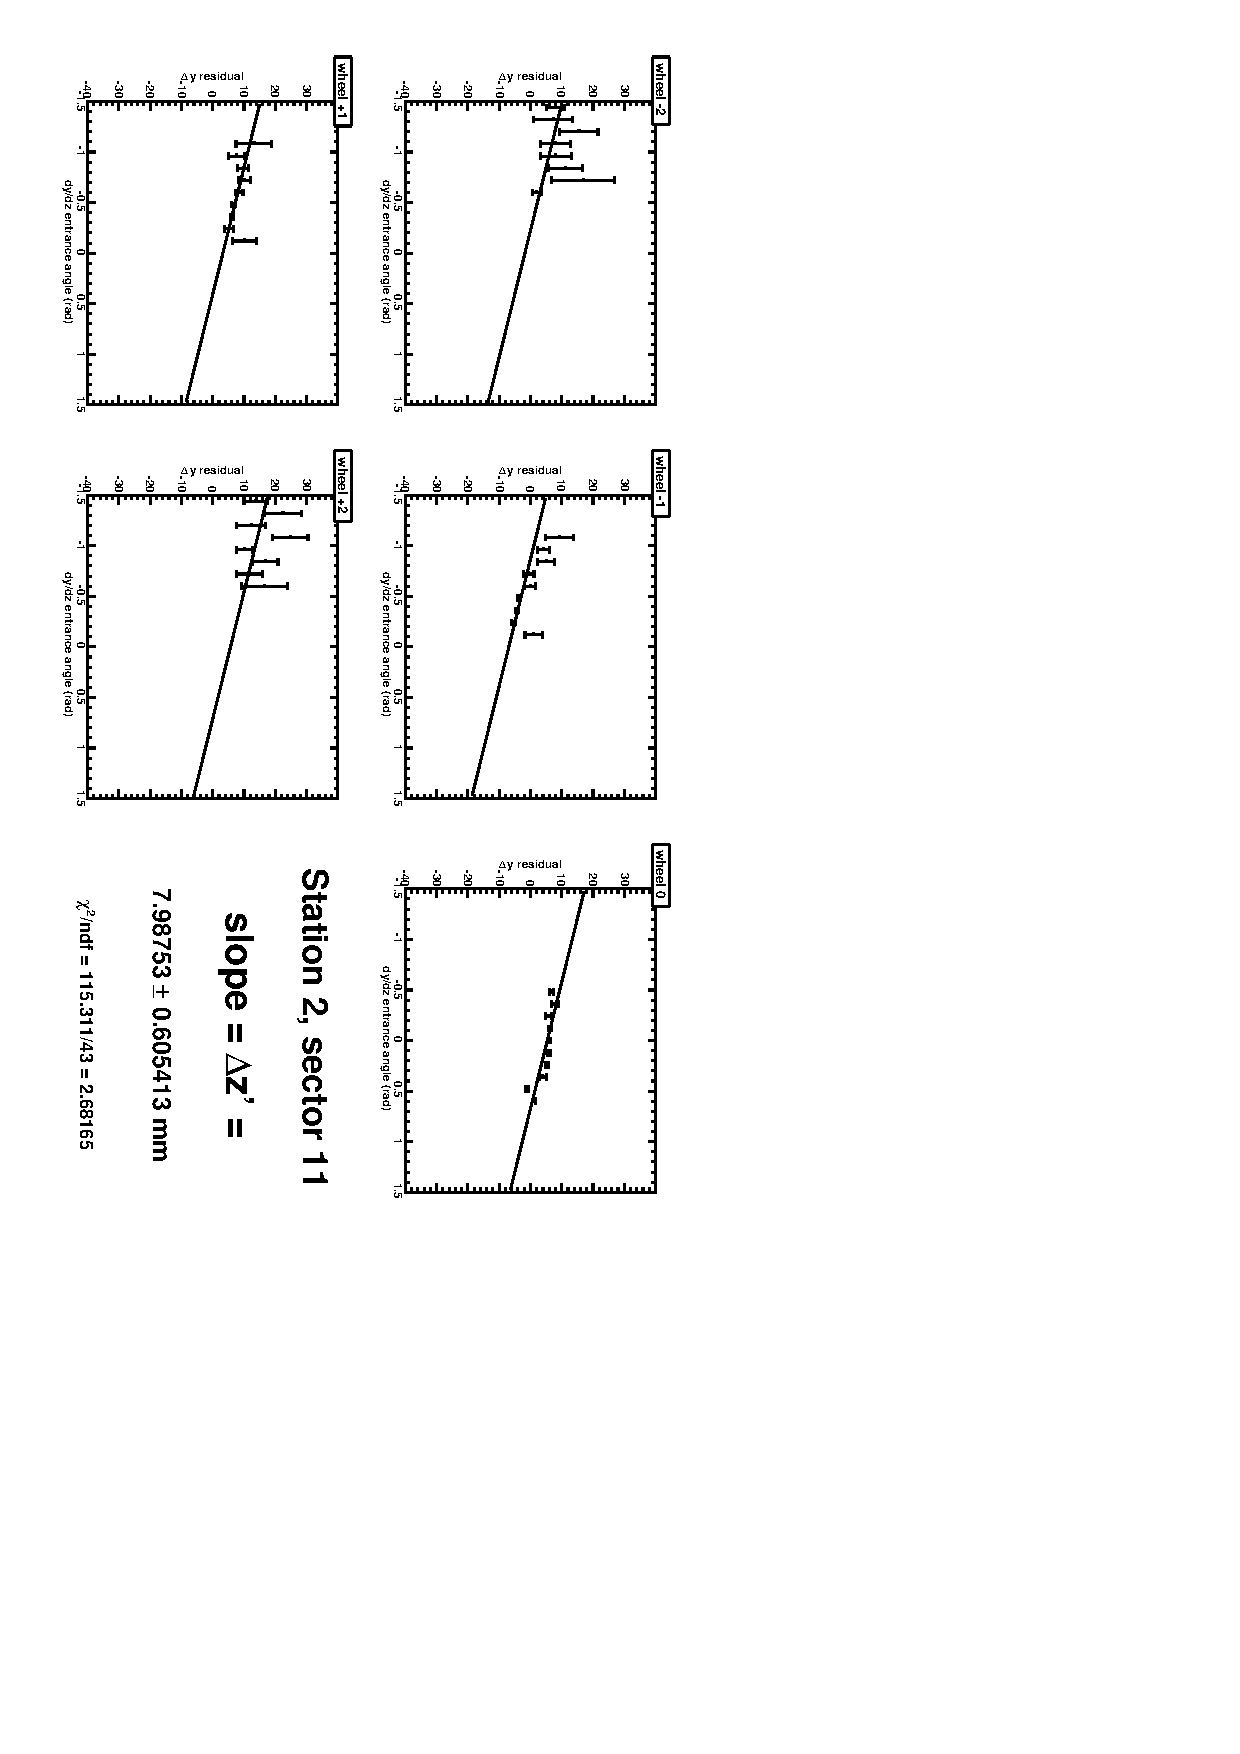
\includegraphics[height=\linewidth, angle=90]{zfits/zfit_2_11.pdf}

\vfill
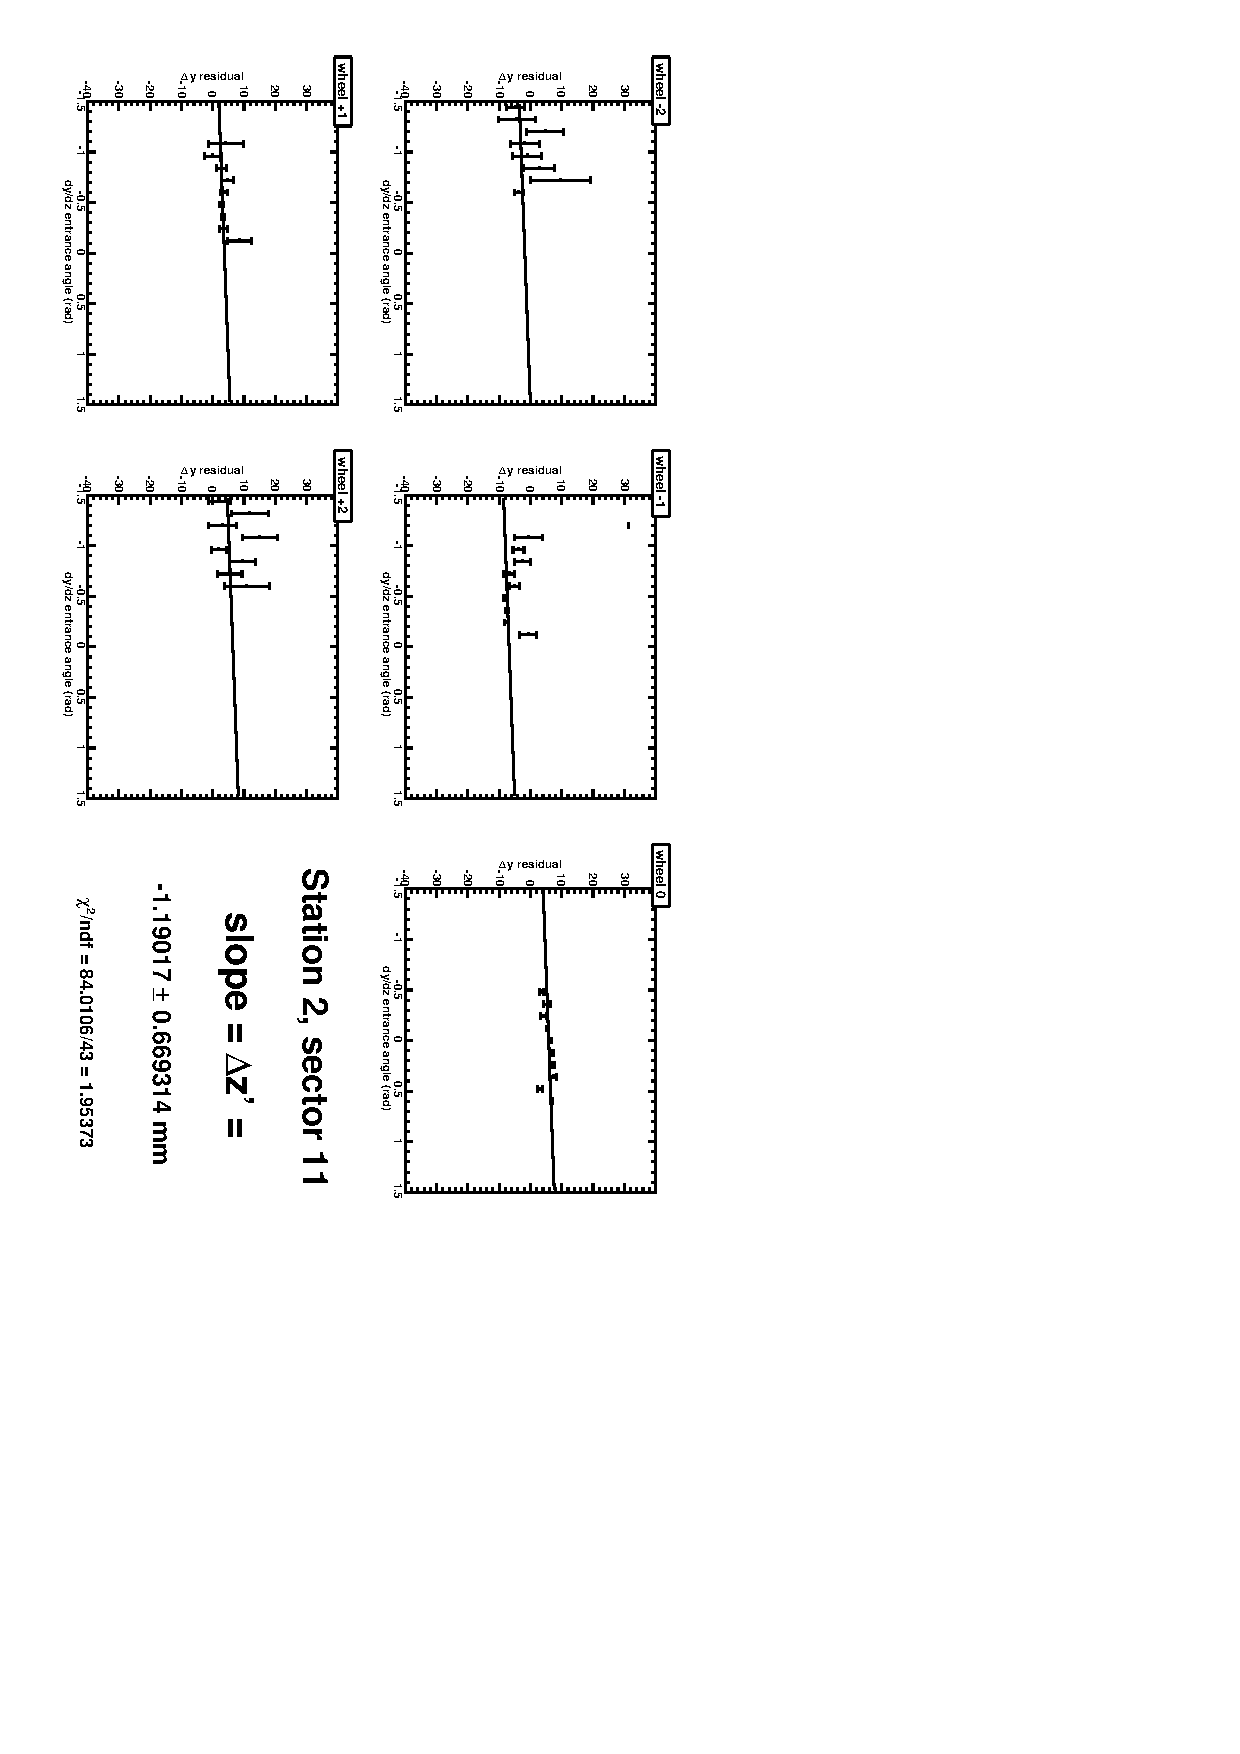
\includegraphics[height=\linewidth, angle=90]{zfits_after/zfit_2_11.pdf}
\column{0.3\linewidth}
\begin{itemize}
\item Top: before \\ Bottom: after
\item Five panels are wheels in the same SemiSuperSector (some are missing)
\item Fit requires all to have the same slope ($\delta_z$), but allows different offsets ($\delta_y$)
\end{itemize}
\end{columns}
\end{frame}

\begin{frame}
\frametitle{Station 2, sector 12}
\begin{columns}
\column{0.7\linewidth}
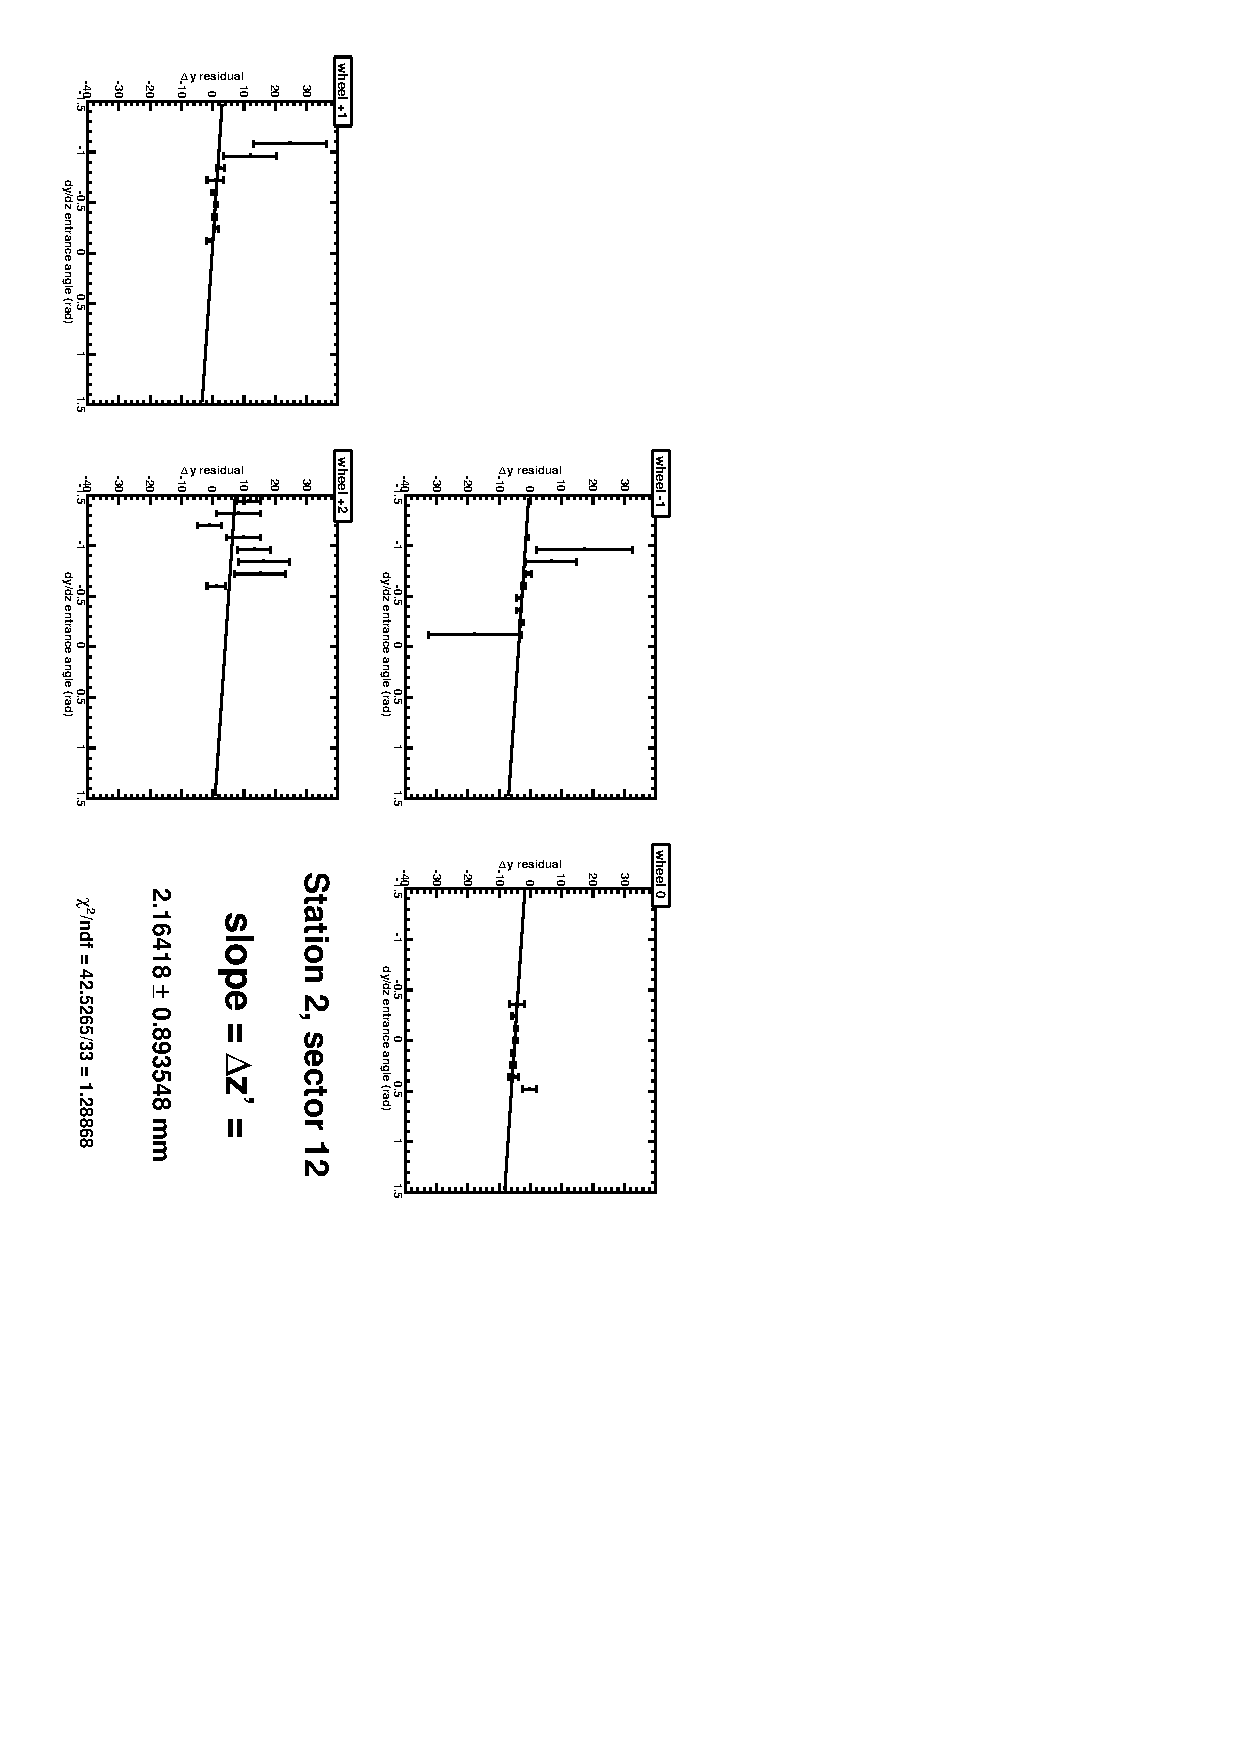
\includegraphics[height=\linewidth, angle=90]{zfits/zfit_2_12.pdf}

\vfill
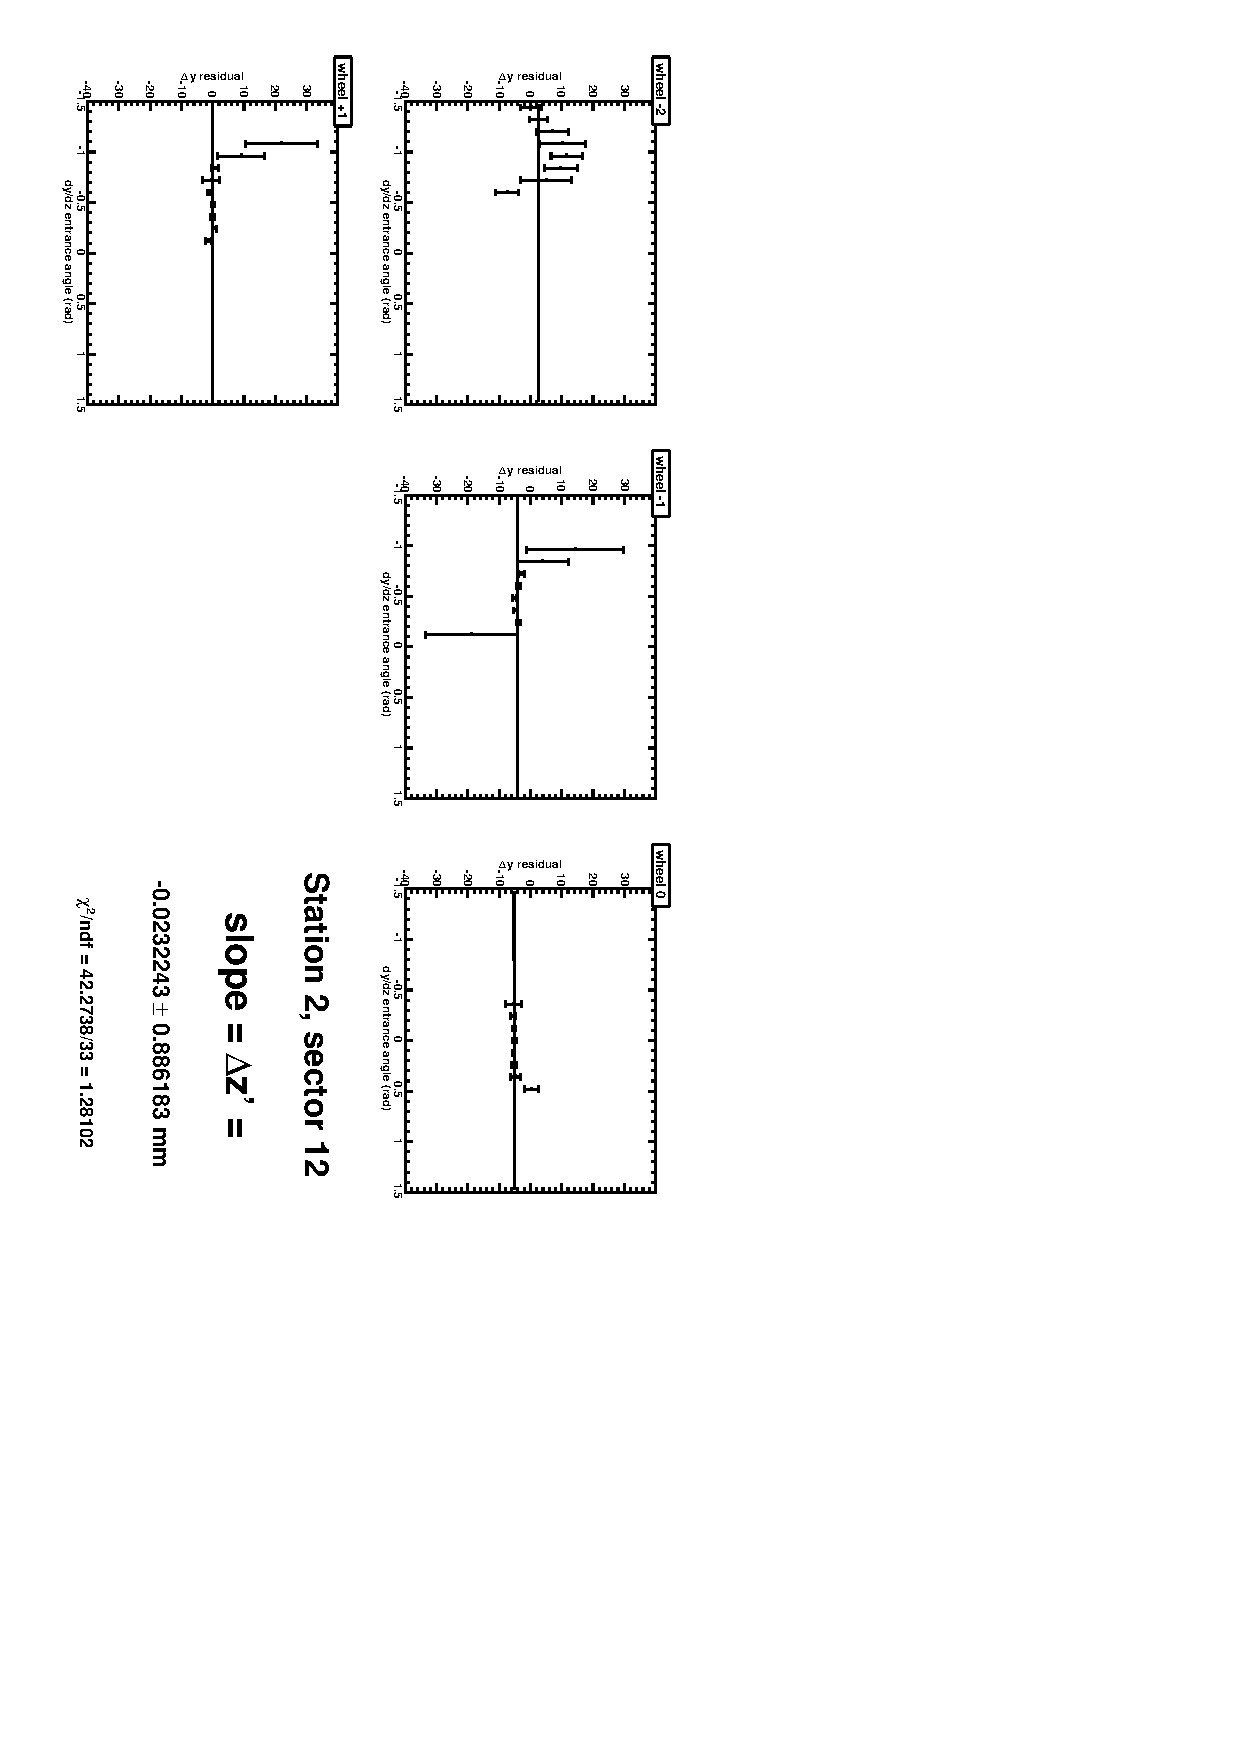
\includegraphics[height=\linewidth, angle=90]{zfits_after/zfit_2_12.pdf}
\column{0.3\linewidth}
\begin{itemize}
\item Top: before \\ Bottom: after
\item Five panels are wheels in the same SemiSuperSector (some are missing)
\item Fit requires all to have the same slope ($\delta_z$), but allows different offsets ($\delta_y$)
\end{itemize}
\end{columns}
\end{frame}

\begin{frame}
\frametitle{Station 3, sector 2}
\begin{columns}
\column{0.7\linewidth}
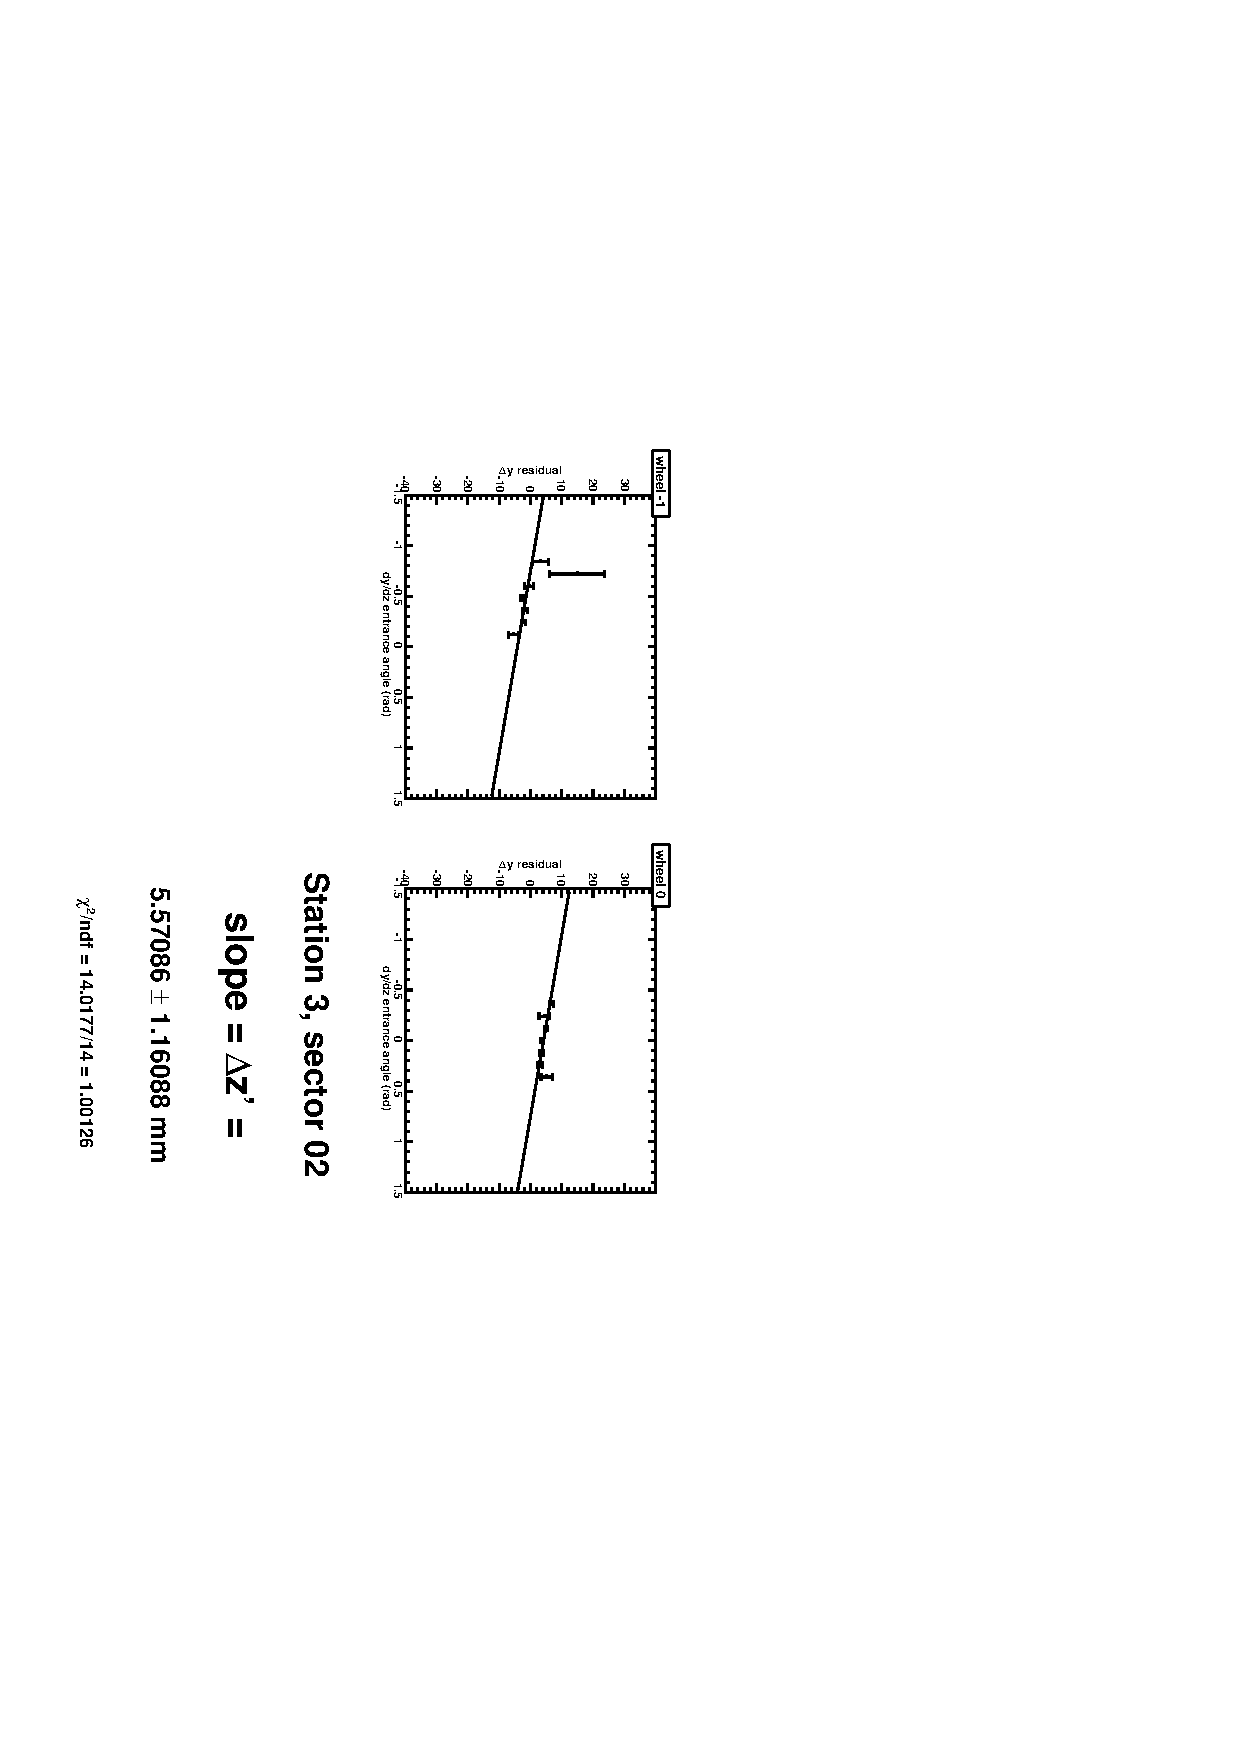
\includegraphics[height=\linewidth, angle=90]{zfits/zfit_3_02.pdf}

\vfill
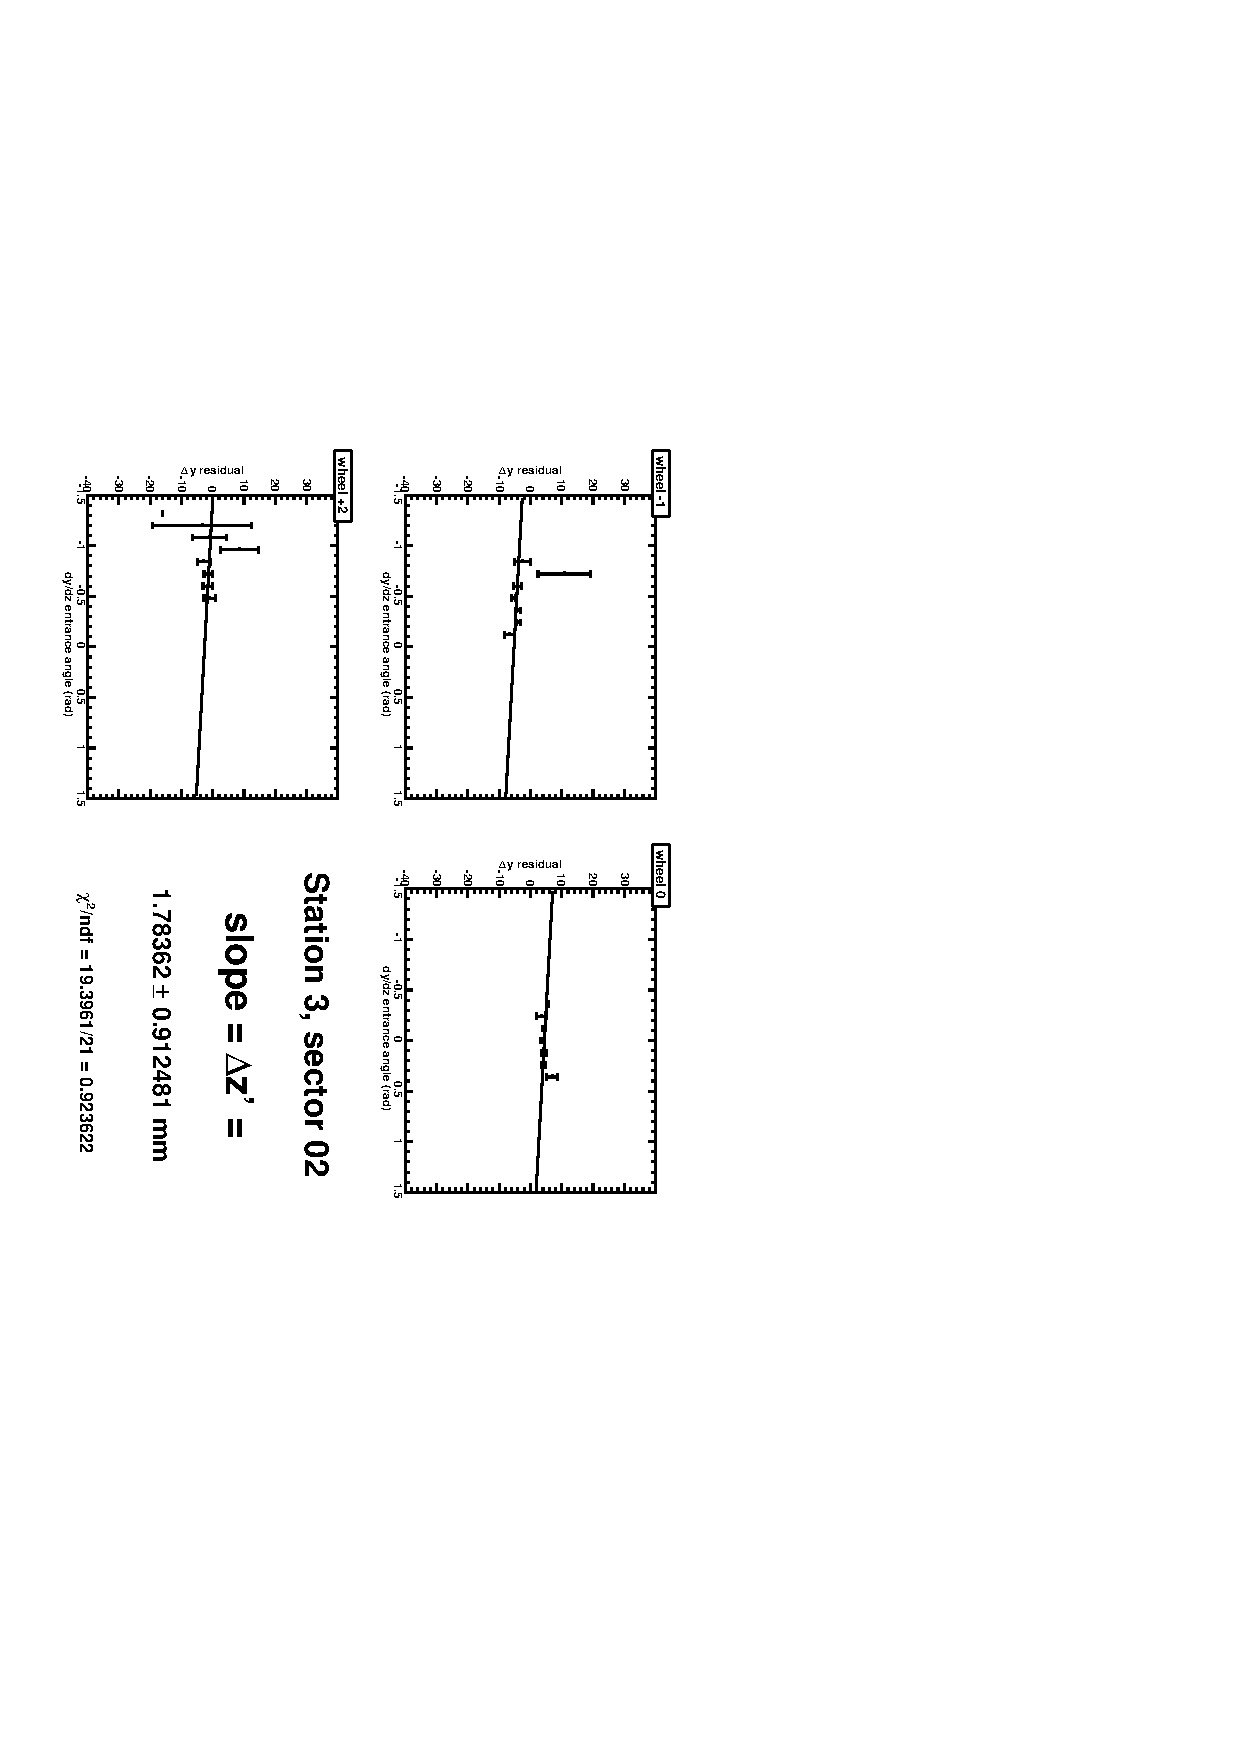
\includegraphics[height=\linewidth, angle=90]{zfits_after/zfit_3_02.pdf}
\column{0.3\linewidth}
\begin{itemize}
\item Top: before \\ Bottom: after
\item Five panels are wheels in the same SemiSuperSector (some are missing)
\item Fit requires all to have the same slope ($\delta_z$), but allows different offsets ($\delta_y$)
\end{itemize}
\end{columns}
\end{frame}

\begin{frame}
\frametitle{Station 3, sector 3}
\begin{columns}
\column{0.7\linewidth}
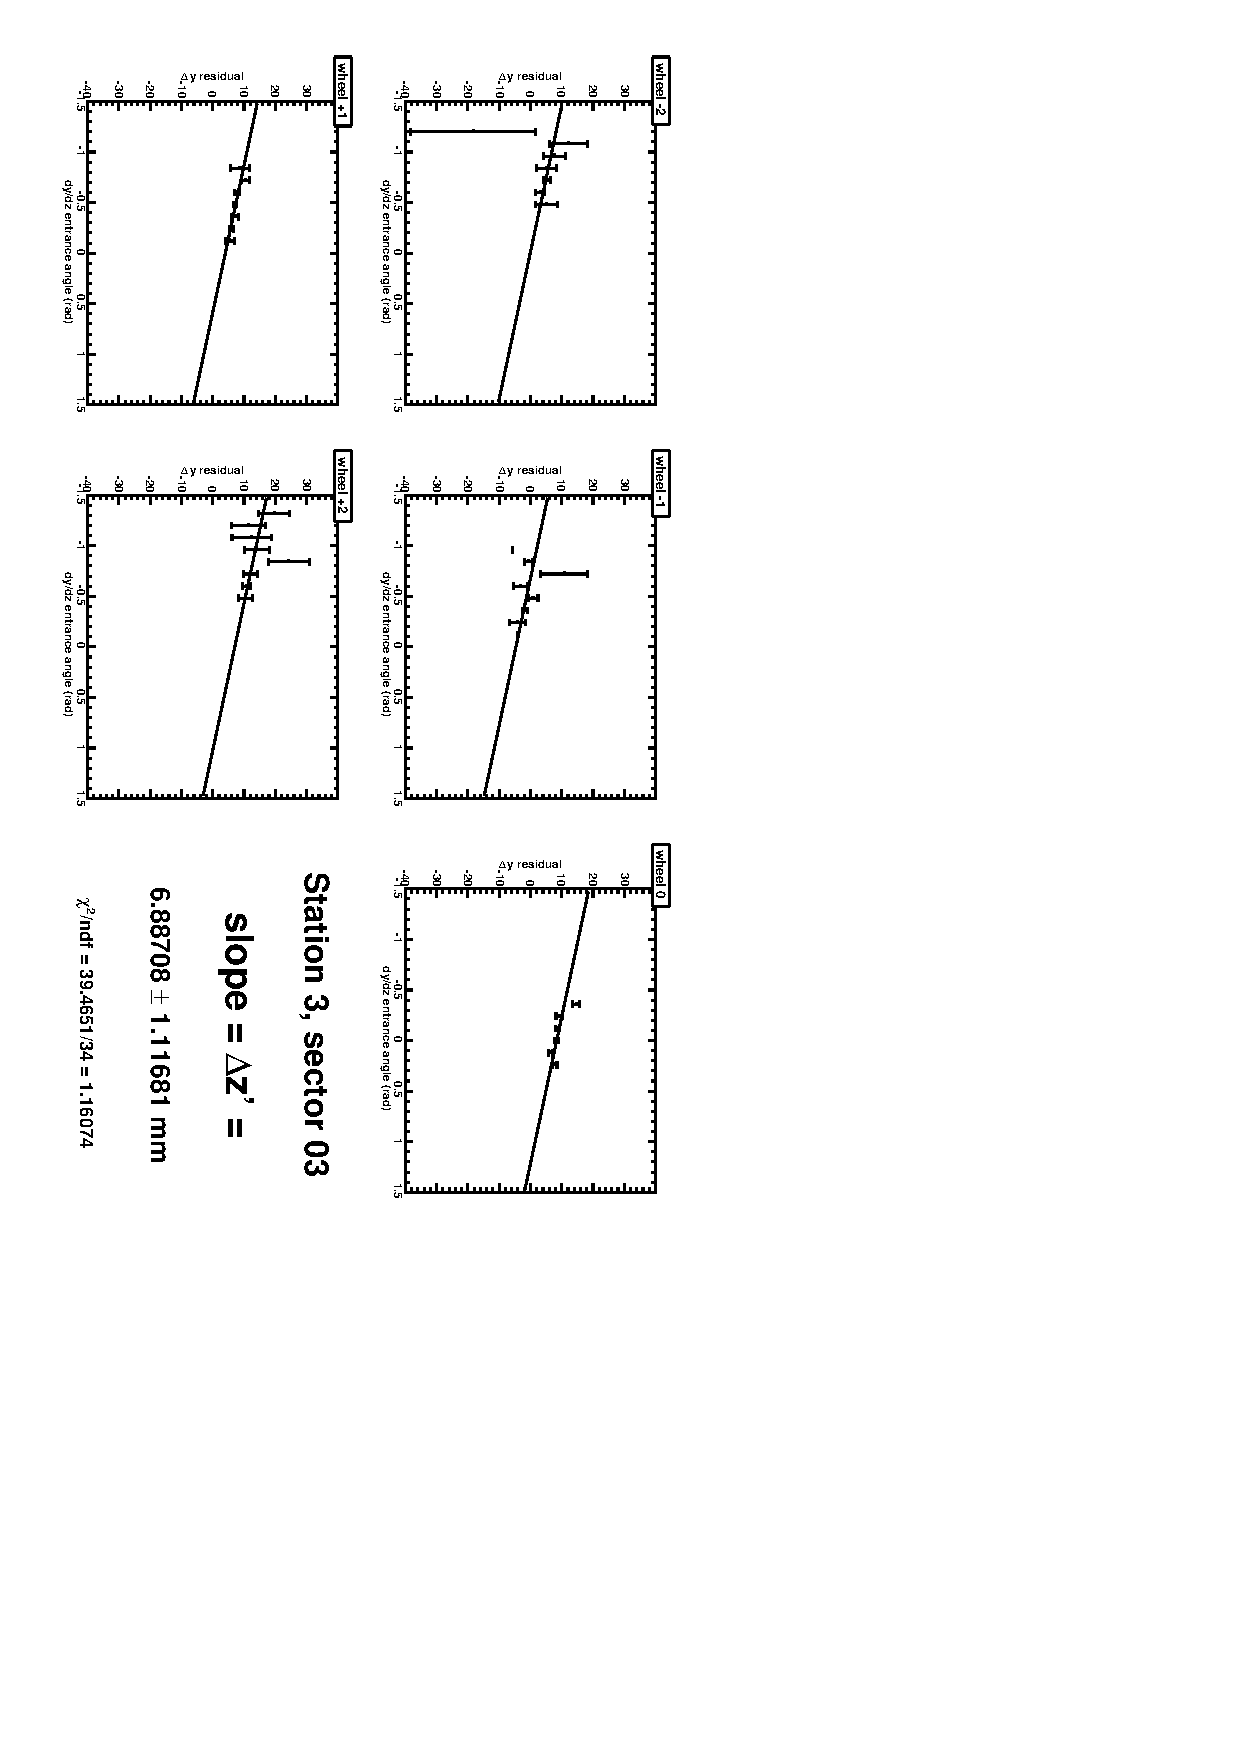
\includegraphics[height=\linewidth, angle=90]{zfits/zfit_3_03.pdf}

\vfill
\includegraphics[height=\linewidth, angle=90]{zfits_after/zfit_3_03.pdf}
\column{0.3\linewidth}
\begin{itemize}
\item Top: before \\ Bottom: after
\item Five panels are wheels in the same SemiSuperSector (some are missing)
\item Fit requires all to have the same slope ($\delta_z$), but allows different offsets ($\delta_y$)
\end{itemize}
\end{columns}
\end{frame}

\begin{frame}
\frametitle{Station 3, sector 4}
\begin{columns}
\column{0.7\linewidth}
\includegraphics[height=\linewidth, angle=90]{zfits/zfit_3_04.pdf}

\vfill
\includegraphics[height=\linewidth, angle=90]{zfits_after/zfit_3_04.pdf}
\column{0.3\linewidth}
\begin{itemize}
\item Top: before \\ Bottom: after
\item Five panels are wheels in the same SemiSuperSector (some are missing)
\item Fit requires all to have the same slope ($\delta_z$), but allows different offsets ($\delta_y$)
\end{itemize}
\end{columns}
\end{frame}

\begin{frame}
\frametitle{Station 3, sector 5}
\begin{columns}
\column{0.7\linewidth}
\includegraphics[height=\linewidth, angle=90]{zfits/zfit_3_05.pdf}

\vfill
\includegraphics[height=\linewidth, angle=90]{zfits_after/zfit_3_05.pdf}
\column{0.3\linewidth}
\begin{itemize}
\item Top: before \\ Bottom: after
\item Five panels are wheels in the same SemiSuperSector (some are missing)
\item Fit requires all to have the same slope ($\delta_z$), but allows different offsets ($\delta_y$)
\end{itemize}
\end{columns}
\end{frame}

\begin{frame}
\frametitle{Station 3, sector 6}
\begin{columns}
\column{0.7\linewidth}
\includegraphics[height=\linewidth, angle=90]{zfits/zfit_3_06.pdf}

\vfill
\includegraphics[height=\linewidth, angle=90]{zfits_after/zfit_3_06.pdf}
\column{0.3\linewidth}
\begin{itemize}
\item Top: before \\ Bottom: after
\item Five panels are wheels in the same SemiSuperSector (some are missing)
\item Fit requires all to have the same slope ($\delta_z$), but allows different offsets ($\delta_y$)
\end{itemize}
\end{columns}
\end{frame}

\begin{frame}
\frametitle{Station 3, sector 7}
\begin{columns}
\column{0.7\linewidth}
\includegraphics[height=\linewidth, angle=90]{zfits/zfit_3_07.pdf}

\vfill
\includegraphics[height=\linewidth, angle=90]{zfits_after/zfit_3_07.pdf}
\column{0.3\linewidth}
\begin{itemize}
\item Top: before \\ Bottom: after
\item Five panels are wheels in the same SemiSuperSector (some are missing)
\item Fit requires all to have the same slope ($\delta_z$), but allows different offsets ($\delta_y$)
\end{itemize}
\end{columns}
\end{frame}

\begin{frame}
\frametitle{Station 3, sector 8}
\begin{columns}
\column{0.7\linewidth}
\includegraphics[height=\linewidth, angle=90]{zfits/zfit_3_08.pdf}

\vfill
\includegraphics[height=\linewidth, angle=90]{zfits_after/zfit_3_08.pdf}
\column{0.3\linewidth}
\begin{itemize}
\item Top: before \\ Bottom: after
\item Five panels are wheels in the same SemiSuperSector (some are missing)
\item Fit requires all to have the same slope ($\delta_z$), but allows different offsets ($\delta_y$)
\end{itemize}
\end{columns}
\end{frame}

\begin{frame}
\frametitle{Station 3, sector 9}
\begin{columns}
\column{0.7\linewidth}
\includegraphics[height=\linewidth, angle=90]{zfits/zfit_3_09.pdf}

\vfill
\includegraphics[height=\linewidth, angle=90]{zfits_after/zfit_3_09.pdf}
\column{0.3\linewidth}
\begin{itemize}
\item Top: before \\ Bottom: after
\item Five panels are wheels in the same SemiSuperSector (some are missing)
\item Fit requires all to have the same slope ($\delta_z$), but allows different offsets ($\delta_y$)
\end{itemize}
\end{columns}
\end{frame}

\begin{frame}
\frametitle{Station 3, sector 10}
\begin{columns}
\column{0.7\linewidth}
\includegraphics[height=\linewidth, angle=90]{zfits/zfit_3_10.pdf}

\vfill
\includegraphics[height=\linewidth, angle=90]{zfits_after/zfit_3_10.pdf}
\column{0.3\linewidth}
\begin{itemize}
\item Top: before \\ Bottom: after
\item Five panels are wheels in the same SemiSuperSector (some are missing)
\item Fit requires all to have the same slope ($\delta_z$), but allows different offsets ($\delta_y$)
\end{itemize}
\end{columns}
\end{frame}

\begin{frame}
\frametitle{Station 3, sector 11}
\begin{columns}
\column{0.7\linewidth}
\includegraphics[height=\linewidth, angle=90]{zfits/zfit_3_11.pdf}

\vfill
\includegraphics[height=\linewidth, angle=90]{zfits_after/zfit_3_11.pdf}
\column{0.3\linewidth}
\begin{itemize}
\item Top: before \\ Bottom: after
\item Five panels are wheels in the same SemiSuperSector (some are missing)
\item Fit requires all to have the same slope ($\delta_z$), but allows different offsets ($\delta_y$)
\end{itemize}
\end{columns}
\end{frame}

\begin{frame}
\frametitle{Station 3, sector 12}
\begin{columns}
\column{0.7\linewidth}
\includegraphics[height=\linewidth, angle=90]{zfits/zfit_3_12.pdf}

\vfill
\includegraphics[height=\linewidth, angle=90]{zfits_after/zfit_3_12.pdf}
\column{0.3\linewidth}
\begin{itemize}
\item Top: before \\ Bottom: after
\item Five panels are wheels in the same SemiSuperSector (some are missing)
\item Fit requires all to have the same slope ($\delta_z$), but allows different offsets ($\delta_y$)
\end{itemize}
\end{columns}
\end{frame}

\begin{frame}
\frametitle{Summary before and after}
\label{after}

\begin{columns}
\column{0.7\linewidth}
\includegraphics[height=\linewidth, angle=90]{zfits_stations.pdf}

\vfill
\includegraphics[height=\linewidth, angle=90]{zfits_stations_2nd.pdf}
\column{0.3\linewidth}
\begin{itemize}
\item Top: plot shown on page~\pageref{summary}
\item Bottom: same thing after applying correction
\item Direction and magnitude are right; could be done with more precision
\end{itemize}
\end{columns}
\end{frame}

\begin{frame}
\frametitle{Consequences for other degrees of freedom}
\begin{itemize}
\item Fix $\delta_z$ to these SemiSuperSector values and run individual chamber alignment.  Below: differences with respect to normal alignment
\item $\delta_z$ are different (naturally: computed with different constraints)
\item $\delta_y$ are different (naturally: alignment matches line-of-sight of tracks and $\frac{dy}{dz}$ is asymmetric in many chambers)
\item Everything else is the same, insensitive to these new $\delta_z$ values
\end{itemize}
\includegraphics[height=0.85\linewidth, angle=90]{zfits_consequence.pdf}
\end{frame}


\begin{frame}
\frametitle{Map plots with SemiSuperSector $\delta_z$}
\includegraphics[width=0.5\linewidth]{zfit_mapplots/DTvsphi_st1whA_x.png}
\includegraphics[width=0.5\linewidth]{zfit_mapplots/DTvsphi_st1whA_y.png}

\includegraphics[width=0.5\linewidth]{zfit_mapplots/DTvsphi_st1whA_dxdz.png}
\includegraphics[width=0.5\linewidth]{zfit_mapplots/DTvsphi_st1whA_dydz.png}
\end{frame}

\begin{frame}
\frametitle{Map plots with SemiSuperSector $\delta_z$}
\includegraphics[width=0.5\linewidth]{zfit_mapplots/DTvsphi_st1whB_x.png}
\includegraphics[width=0.5\linewidth]{zfit_mapplots/DTvsphi_st1whB_y.png}

\includegraphics[width=0.5\linewidth]{zfit_mapplots/DTvsphi_st1whB_dxdz.png}
\includegraphics[width=0.5\linewidth]{zfit_mapplots/DTvsphi_st1whB_dydz.png}
\end{frame}

\begin{frame}
\frametitle{Map plots with SemiSuperSector $\delta_z$}
\includegraphics[width=0.5\linewidth]{zfit_mapplots/DTvsphi_st1whC_x.png}
\includegraphics[width=0.5\linewidth]{zfit_mapplots/DTvsphi_st1whC_y.png}

\includegraphics[width=0.5\linewidth]{zfit_mapplots/DTvsphi_st1whC_dxdz.png}
\includegraphics[width=0.5\linewidth]{zfit_mapplots/DTvsphi_st1whC_dydz.png}
\end{frame}

\begin{frame}
\frametitle{Map plots with SemiSuperSector $\delta_z$}
\includegraphics[width=0.5\linewidth]{zfit_mapplots/DTvsphi_st1whD_x.png}
\includegraphics[width=0.5\linewidth]{zfit_mapplots/DTvsphi_st1whD_y.png}

\includegraphics[width=0.5\linewidth]{zfit_mapplots/DTvsphi_st1whD_dxdz.png}
\includegraphics[width=0.5\linewidth]{zfit_mapplots/DTvsphi_st1whD_dydz.png}
\end{frame}

\begin{frame}
\frametitle{Map plots with SemiSuperSector $\delta_z$}
\includegraphics[width=0.5\linewidth]{zfit_mapplots/DTvsphi_st1whE_x.png}
\includegraphics[width=0.5\linewidth]{zfit_mapplots/DTvsphi_st1whE_y.png}

\includegraphics[width=0.5\linewidth]{zfit_mapplots/DTvsphi_st1whE_dxdz.png}
\includegraphics[width=0.5\linewidth]{zfit_mapplots/DTvsphi_st1whE_dydz.png}
\end{frame}

\begin{frame}
\frametitle{Map plots with SemiSuperSector $\delta_z$}
\includegraphics[width=0.5\linewidth]{zfit_mapplots/DTvsphi_st2whA_x.png}
\includegraphics[width=0.5\linewidth]{zfit_mapplots/DTvsphi_st2whA_y.png}

\includegraphics[width=0.5\linewidth]{zfit_mapplots/DTvsphi_st2whA_dxdz.png}
\includegraphics[width=0.5\linewidth]{zfit_mapplots/DTvsphi_st2whA_dydz.png}
\end{frame}

\begin{frame}
\frametitle{Map plots with SemiSuperSector $\delta_z$}
\includegraphics[width=0.5\linewidth]{zfit_mapplots/DTvsphi_st2whB_x.png}
\includegraphics[width=0.5\linewidth]{zfit_mapplots/DTvsphi_st2whB_y.png}

\includegraphics[width=0.5\linewidth]{zfit_mapplots/DTvsphi_st2whB_dxdz.png}
\includegraphics[width=0.5\linewidth]{zfit_mapplots/DTvsphi_st2whB_dydz.png}
\end{frame}

\begin{frame}
\frametitle{Map plots with SemiSuperSector $\delta_z$}
\includegraphics[width=0.5\linewidth]{zfit_mapplots/DTvsphi_st2whC_x.png}
\includegraphics[width=0.5\linewidth]{zfit_mapplots/DTvsphi_st2whC_y.png}

\includegraphics[width=0.5\linewidth]{zfit_mapplots/DTvsphi_st2whC_dxdz.png}
\includegraphics[width=0.5\linewidth]{zfit_mapplots/DTvsphi_st2whC_dydz.png}
\end{frame}

\begin{frame}
\frametitle{Map plots with SemiSuperSector $\delta_z$}
\includegraphics[width=0.5\linewidth]{zfit_mapplots/DTvsphi_st2whD_x.png}
\includegraphics[width=0.5\linewidth]{zfit_mapplots/DTvsphi_st2whD_y.png}

\includegraphics[width=0.5\linewidth]{zfit_mapplots/DTvsphi_st2whD_dxdz.png}
\includegraphics[width=0.5\linewidth]{zfit_mapplots/DTvsphi_st2whD_dydz.png}
\end{frame}

\begin{frame}
\frametitle{Map plots with SemiSuperSector $\delta_z$}
\includegraphics[width=0.5\linewidth]{zfit_mapplots/DTvsphi_st2whE_x.png}
\includegraphics[width=0.5\linewidth]{zfit_mapplots/DTvsphi_st2whE_y.png}

\includegraphics[width=0.5\linewidth]{zfit_mapplots/DTvsphi_st2whE_dxdz.png}
\includegraphics[width=0.5\linewidth]{zfit_mapplots/DTvsphi_st2whE_dydz.png}
\end{frame}

\begin{frame}
\frametitle{Map plots with SemiSuperSector $\delta_z$}
\includegraphics[width=0.5\linewidth]{zfit_mapplots/DTvsphi_st3whA_x.png}
\includegraphics[width=0.5\linewidth]{zfit_mapplots/DTvsphi_st3whA_y.png}

\includegraphics[width=0.5\linewidth]{zfit_mapplots/DTvsphi_st3whA_dxdz.png}
\includegraphics[width=0.5\linewidth]{zfit_mapplots/DTvsphi_st3whA_dydz.png}
\end{frame}

\begin{frame}
\frametitle{Map plots with SemiSuperSector $\delta_z$}
\includegraphics[width=0.5\linewidth]{zfit_mapplots/DTvsphi_st3whB_x.png}
\includegraphics[width=0.5\linewidth]{zfit_mapplots/DTvsphi_st3whB_y.png}

\includegraphics[width=0.5\linewidth]{zfit_mapplots/DTvsphi_st3whB_dxdz.png}
\includegraphics[width=0.5\linewidth]{zfit_mapplots/DTvsphi_st3whB_dydz.png}
\end{frame}

\begin{frame}
\frametitle{Map plots with SemiSuperSector $\delta_z$}
\includegraphics[width=0.5\linewidth]{zfit_mapplots/DTvsphi_st3whC_x.png}
\includegraphics[width=0.5\linewidth]{zfit_mapplots/DTvsphi_st3whC_y.png}

\includegraphics[width=0.5\linewidth]{zfit_mapplots/DTvsphi_st3whC_dxdz.png}
\includegraphics[width=0.5\linewidth]{zfit_mapplots/DTvsphi_st3whC_dydz.png}
\end{frame}

\begin{frame}
\frametitle{Map plots with SemiSuperSector $\delta_z$}
\includegraphics[width=0.5\linewidth]{zfit_mapplots/DTvsphi_st3whD_x.png}
\includegraphics[width=0.5\linewidth]{zfit_mapplots/DTvsphi_st3whD_y.png}

\includegraphics[width=0.5\linewidth]{zfit_mapplots/DTvsphi_st3whD_dxdz.png}
\includegraphics[width=0.5\linewidth]{zfit_mapplots/DTvsphi_st3whD_dydz.png}
\end{frame}

\begin{frame}
\frametitle{Map plots with SemiSuperSector $\delta_z$}
\includegraphics[width=0.5\linewidth]{zfit_mapplots/DTvsphi_st3whE_x.png}
\includegraphics[width=0.5\linewidth]{zfit_mapplots/DTvsphi_st3whE_y.png}

\includegraphics[width=0.5\linewidth]{zfit_mapplots/DTvsphi_st3whE_dxdz.png}
\includegraphics[width=0.5\linewidth]{zfit_mapplots/DTvsphi_st3whE_dydz.png}
\end{frame}

\begin{frame}
\frametitle{Map plots with SemiSuperSector $\delta_z$}
\includegraphics[width=0.5\linewidth]{zfit_mapplots/DTvsphi_st4whA_x.png}

\includegraphics[width=0.5\linewidth]{zfit_mapplots/DTvsphi_st4whA_dxdz.png}
\end{frame}

\begin{frame}
\frametitle{Map plots with SemiSuperSector $\delta_z$}
\includegraphics[width=0.5\linewidth]{zfit_mapplots/DTvsphi_st4whB_x.png}

\includegraphics[width=0.5\linewidth]{zfit_mapplots/DTvsphi_st4whB_dxdz.png}
\end{frame}

\begin{frame}
\frametitle{Map plots with SemiSuperSector $\delta_z$}
\includegraphics[width=0.5\linewidth]{zfit_mapplots/DTvsphi_st4whC_x.png}

\includegraphics[width=0.5\linewidth]{zfit_mapplots/DTvsphi_st4whC_dxdz.png}
\end{frame}

\begin{frame}
\frametitle{Map plots with SemiSuperSector $\delta_z$}
\includegraphics[width=0.5\linewidth]{zfit_mapplots/DTvsphi_st4whD_x.png}

\includegraphics[width=0.5\linewidth]{zfit_mapplots/DTvsphi_st4whD_dxdz.png}
\end{frame}

\begin{frame}
\frametitle{Map plots with SemiSuperSector $\delta_z$}
\includegraphics[width=0.5\linewidth]{zfit_mapplots/DTvsphi_st4whE_x.png}

\includegraphics[width=0.5\linewidth]{zfit_mapplots/DTvsphi_st4whE_dxdz.png}
\end{frame}

\begin{frame}
\frametitle{Map plots with SemiSuperSector $\delta_z$}
\includegraphics[width=0.5\linewidth]{zfit_mapplots/DTvsz_st1sec01_x.png}
\includegraphics[width=0.5\linewidth]{zfit_mapplots/DTvsz_st1sec01_y.png}

\includegraphics[width=0.5\linewidth]{zfit_mapplots/DTvsz_st1sec01_dxdz.png}
\includegraphics[width=0.5\linewidth]{zfit_mapplots/DTvsz_st1sec01_dydz.png}
\end{frame}

\begin{frame}
\frametitle{Map plots with SemiSuperSector $\delta_z$}
\includegraphics[width=0.5\linewidth]{zfit_mapplots/DTvsz_st1sec02_x.png}
\includegraphics[width=0.5\linewidth]{zfit_mapplots/DTvsz_st1sec02_y.png}

\includegraphics[width=0.5\linewidth]{zfit_mapplots/DTvsz_st1sec02_dxdz.png}
\includegraphics[width=0.5\linewidth]{zfit_mapplots/DTvsz_st1sec02_dydz.png}
\end{frame}

\begin{frame}
\frametitle{Map plots with SemiSuperSector $\delta_z$}
\includegraphics[width=0.5\linewidth]{zfit_mapplots/DTvsz_st1sec03_x.png}
\includegraphics[width=0.5\linewidth]{zfit_mapplots/DTvsz_st1sec03_y.png}

\includegraphics[width=0.5\linewidth]{zfit_mapplots/DTvsz_st1sec03_dxdz.png}
\includegraphics[width=0.5\linewidth]{zfit_mapplots/DTvsz_st1sec03_dydz.png}
\end{frame}

\begin{frame}
\frametitle{Map plots with SemiSuperSector $\delta_z$}
\includegraphics[width=0.5\linewidth]{zfit_mapplots/DTvsz_st1sec04_x.png}
\includegraphics[width=0.5\linewidth]{zfit_mapplots/DTvsz_st1sec04_y.png}

\includegraphics[width=0.5\linewidth]{zfit_mapplots/DTvsz_st1sec04_dxdz.png}
\includegraphics[width=0.5\linewidth]{zfit_mapplots/DTvsz_st1sec04_dydz.png}
\end{frame}

\begin{frame}
\frametitle{Map plots with SemiSuperSector $\delta_z$}
\includegraphics[width=0.5\linewidth]{zfit_mapplots/DTvsz_st1sec05_x.png}
\includegraphics[width=0.5\linewidth]{zfit_mapplots/DTvsz_st1sec05_y.png}

\includegraphics[width=0.5\linewidth]{zfit_mapplots/DTvsz_st1sec05_dxdz.png}
\includegraphics[width=0.5\linewidth]{zfit_mapplots/DTvsz_st1sec05_dydz.png}
\end{frame}

\begin{frame}
\frametitle{Map plots with SemiSuperSector $\delta_z$}
\includegraphics[width=0.5\linewidth]{zfit_mapplots/DTvsz_st1sec06_x.png}
\includegraphics[width=0.5\linewidth]{zfit_mapplots/DTvsz_st1sec06_y.png}

\includegraphics[width=0.5\linewidth]{zfit_mapplots/DTvsz_st1sec06_dxdz.png}
\includegraphics[width=0.5\linewidth]{zfit_mapplots/DTvsz_st1sec06_dydz.png}
\end{frame}

\begin{frame}
\frametitle{Map plots with SemiSuperSector $\delta_z$}
\includegraphics[width=0.5\linewidth]{zfit_mapplots/DTvsz_st1sec07_x.png}
\includegraphics[width=0.5\linewidth]{zfit_mapplots/DTvsz_st1sec07_y.png}

\includegraphics[width=0.5\linewidth]{zfit_mapplots/DTvsz_st1sec07_dxdz.png}
\includegraphics[width=0.5\linewidth]{zfit_mapplots/DTvsz_st1sec07_dydz.png}
\end{frame}

\begin{frame}
\frametitle{Map plots with SemiSuperSector $\delta_z$}
\includegraphics[width=0.5\linewidth]{zfit_mapplots/DTvsz_st1sec08_x.png}
\includegraphics[width=0.5\linewidth]{zfit_mapplots/DTvsz_st1sec08_y.png}

\includegraphics[width=0.5\linewidth]{zfit_mapplots/DTvsz_st1sec08_dxdz.png}
\includegraphics[width=0.5\linewidth]{zfit_mapplots/DTvsz_st1sec08_dydz.png}
\end{frame}

\begin{frame}
\frametitle{Map plots with SemiSuperSector $\delta_z$}
\includegraphics[width=0.5\linewidth]{zfit_mapplots/DTvsz_st1sec09_x.png}
\includegraphics[width=0.5\linewidth]{zfit_mapplots/DTvsz_st1sec09_y.png}

\includegraphics[width=0.5\linewidth]{zfit_mapplots/DTvsz_st1sec09_dxdz.png}
\includegraphics[width=0.5\linewidth]{zfit_mapplots/DTvsz_st1sec09_dydz.png}
\end{frame}

\begin{frame}
\frametitle{Map plots with SemiSuperSector $\delta_z$}
\includegraphics[width=0.5\linewidth]{zfit_mapplots/DTvsz_st1sec10_x.png}
\includegraphics[width=0.5\linewidth]{zfit_mapplots/DTvsz_st1sec10_y.png}

\includegraphics[width=0.5\linewidth]{zfit_mapplots/DTvsz_st1sec10_dxdz.png}
\includegraphics[width=0.5\linewidth]{zfit_mapplots/DTvsz_st1sec10_dydz.png}
\end{frame}

\begin{frame}
\frametitle{Map plots with SemiSuperSector $\delta_z$}
\includegraphics[width=0.5\linewidth]{zfit_mapplots/DTvsz_st1sec11_x.png}
\includegraphics[width=0.5\linewidth]{zfit_mapplots/DTvsz_st1sec11_y.png}

\includegraphics[width=0.5\linewidth]{zfit_mapplots/DTvsz_st1sec11_dxdz.png}
\includegraphics[width=0.5\linewidth]{zfit_mapplots/DTvsz_st1sec11_dydz.png}
\end{frame}

\begin{frame}
\frametitle{Map plots with SemiSuperSector $\delta_z$}
\includegraphics[width=0.5\linewidth]{zfit_mapplots/DTvsz_st1sec12_x.png}
\includegraphics[width=0.5\linewidth]{zfit_mapplots/DTvsz_st1sec12_y.png}

\includegraphics[width=0.5\linewidth]{zfit_mapplots/DTvsz_st1sec12_dxdz.png}
\includegraphics[width=0.5\linewidth]{zfit_mapplots/DTvsz_st1sec12_dydz.png}
\end{frame}

\begin{frame}
\frametitle{Map plots with SemiSuperSector $\delta_z$}
\includegraphics[width=0.5\linewidth]{zfit_mapplots/DTvsz_st2sec01_x.png}
\includegraphics[width=0.5\linewidth]{zfit_mapplots/DTvsz_st2sec01_y.png}

\includegraphics[width=0.5\linewidth]{zfit_mapplots/DTvsz_st2sec01_dxdz.png}
\includegraphics[width=0.5\linewidth]{zfit_mapplots/DTvsz_st2sec01_dydz.png}
\end{frame}

\begin{frame}
\frametitle{Map plots with SemiSuperSector $\delta_z$}
\includegraphics[width=0.5\linewidth]{zfit_mapplots/DTvsz_st2sec02_x.png}
\includegraphics[width=0.5\linewidth]{zfit_mapplots/DTvsz_st2sec02_y.png}

\includegraphics[width=0.5\linewidth]{zfit_mapplots/DTvsz_st2sec02_dxdz.png}
\includegraphics[width=0.5\linewidth]{zfit_mapplots/DTvsz_st2sec02_dydz.png}
\end{frame}

\begin{frame}
\frametitle{Map plots with SemiSuperSector $\delta_z$}
\includegraphics[width=0.5\linewidth]{zfit_mapplots/DTvsz_st2sec03_x.png}
\includegraphics[width=0.5\linewidth]{zfit_mapplots/DTvsz_st2sec03_y.png}

\includegraphics[width=0.5\linewidth]{zfit_mapplots/DTvsz_st2sec03_dxdz.png}
\includegraphics[width=0.5\linewidth]{zfit_mapplots/DTvsz_st2sec03_dydz.png}
\end{frame}

\begin{frame}
\frametitle{Map plots with SemiSuperSector $\delta_z$}
\includegraphics[width=0.5\linewidth]{zfit_mapplots/DTvsz_st2sec04_x.png}
\includegraphics[width=0.5\linewidth]{zfit_mapplots/DTvsz_st2sec04_y.png}

\includegraphics[width=0.5\linewidth]{zfit_mapplots/DTvsz_st2sec04_dxdz.png}
\includegraphics[width=0.5\linewidth]{zfit_mapplots/DTvsz_st2sec04_dydz.png}
\end{frame}

\begin{frame}
\frametitle{Map plots with SemiSuperSector $\delta_z$}
\includegraphics[width=0.5\linewidth]{zfit_mapplots/DTvsz_st2sec05_x.png}
\includegraphics[width=0.5\linewidth]{zfit_mapplots/DTvsz_st2sec05_y.png}

\includegraphics[width=0.5\linewidth]{zfit_mapplots/DTvsz_st2sec05_dxdz.png}
\includegraphics[width=0.5\linewidth]{zfit_mapplots/DTvsz_st2sec05_dydz.png}
\end{frame}

\begin{frame}
\frametitle{Map plots with SemiSuperSector $\delta_z$}
\includegraphics[width=0.5\linewidth]{zfit_mapplots/DTvsz_st2sec06_x.png}
\includegraphics[width=0.5\linewidth]{zfit_mapplots/DTvsz_st2sec06_y.png}

\includegraphics[width=0.5\linewidth]{zfit_mapplots/DTvsz_st2sec06_dxdz.png}
\includegraphics[width=0.5\linewidth]{zfit_mapplots/DTvsz_st2sec06_dydz.png}
\end{frame}

\begin{frame}
\frametitle{Map plots with SemiSuperSector $\delta_z$}
\includegraphics[width=0.5\linewidth]{zfit_mapplots/DTvsz_st2sec07_x.png}
\includegraphics[width=0.5\linewidth]{zfit_mapplots/DTvsz_st2sec07_y.png}

\includegraphics[width=0.5\linewidth]{zfit_mapplots/DTvsz_st2sec07_dxdz.png}
\includegraphics[width=0.5\linewidth]{zfit_mapplots/DTvsz_st2sec07_dydz.png}
\end{frame}

\begin{frame}
\frametitle{Map plots with SemiSuperSector $\delta_z$}
\includegraphics[width=0.5\linewidth]{zfit_mapplots/DTvsz_st2sec08_x.png}
\includegraphics[width=0.5\linewidth]{zfit_mapplots/DTvsz_st2sec08_y.png}

\includegraphics[width=0.5\linewidth]{zfit_mapplots/DTvsz_st2sec08_dxdz.png}
\includegraphics[width=0.5\linewidth]{zfit_mapplots/DTvsz_st2sec08_dydz.png}
\end{frame}

\begin{frame}
\frametitle{Map plots with SemiSuperSector $\delta_z$}
\includegraphics[width=0.5\linewidth]{zfit_mapplots/DTvsz_st2sec09_x.png}
\includegraphics[width=0.5\linewidth]{zfit_mapplots/DTvsz_st2sec09_y.png}

\includegraphics[width=0.5\linewidth]{zfit_mapplots/DTvsz_st2sec09_dxdz.png}
\includegraphics[width=0.5\linewidth]{zfit_mapplots/DTvsz_st2sec09_dydz.png}
\end{frame}

\begin{frame}
\frametitle{Map plots with SemiSuperSector $\delta_z$}
\includegraphics[width=0.5\linewidth]{zfit_mapplots/DTvsz_st2sec10_x.png}
\includegraphics[width=0.5\linewidth]{zfit_mapplots/DTvsz_st2sec10_y.png}

\includegraphics[width=0.5\linewidth]{zfit_mapplots/DTvsz_st2sec10_dxdz.png}
\includegraphics[width=0.5\linewidth]{zfit_mapplots/DTvsz_st2sec10_dydz.png}
\end{frame}

\begin{frame}
\frametitle{Map plots with SemiSuperSector $\delta_z$}
\includegraphics[width=0.5\linewidth]{zfit_mapplots/DTvsz_st2sec11_x.png}
\includegraphics[width=0.5\linewidth]{zfit_mapplots/DTvsz_st2sec11_y.png}

\includegraphics[width=0.5\linewidth]{zfit_mapplots/DTvsz_st2sec11_dxdz.png}
\includegraphics[width=0.5\linewidth]{zfit_mapplots/DTvsz_st2sec11_dydz.png}
\end{frame}

\begin{frame}
\frametitle{Map plots with SemiSuperSector $\delta_z$}
\includegraphics[width=0.5\linewidth]{zfit_mapplots/DTvsz_st2sec12_x.png}
\includegraphics[width=0.5\linewidth]{zfit_mapplots/DTvsz_st2sec12_y.png}

\includegraphics[width=0.5\linewidth]{zfit_mapplots/DTvsz_st2sec12_dxdz.png}
\includegraphics[width=0.5\linewidth]{zfit_mapplots/DTvsz_st2sec12_dydz.png}
\end{frame}

\begin{frame}
\frametitle{Map plots with SemiSuperSector $\delta_z$}
\includegraphics[width=0.5\linewidth]{zfit_mapplots/DTvsz_st3sec01_x.png}
\includegraphics[width=0.5\linewidth]{zfit_mapplots/DTvsz_st3sec01_y.png}

\includegraphics[width=0.5\linewidth]{zfit_mapplots/DTvsz_st3sec01_dxdz.png}
\includegraphics[width=0.5\linewidth]{zfit_mapplots/DTvsz_st3sec01_dydz.png}
\end{frame}

\begin{frame}
\frametitle{Map plots with SemiSuperSector $\delta_z$}
\includegraphics[width=0.5\linewidth]{zfit_mapplots/DTvsz_st3sec02_x.png}
\includegraphics[width=0.5\linewidth]{zfit_mapplots/DTvsz_st3sec02_y.png}

\includegraphics[width=0.5\linewidth]{zfit_mapplots/DTvsz_st3sec02_dxdz.png}
\includegraphics[width=0.5\linewidth]{zfit_mapplots/DTvsz_st3sec02_dydz.png}
\end{frame}

\begin{frame}
\frametitle{Map plots with SemiSuperSector $\delta_z$}
\includegraphics[width=0.5\linewidth]{zfit_mapplots/DTvsz_st3sec03_x.png}
\includegraphics[width=0.5\linewidth]{zfit_mapplots/DTvsz_st3sec03_y.png}

\includegraphics[width=0.5\linewidth]{zfit_mapplots/DTvsz_st3sec03_dxdz.png}
\includegraphics[width=0.5\linewidth]{zfit_mapplots/DTvsz_st3sec03_dydz.png}
\end{frame}

\begin{frame}
\frametitle{Map plots with SemiSuperSector $\delta_z$}
\includegraphics[width=0.5\linewidth]{zfit_mapplots/DTvsz_st3sec04_x.png}
\includegraphics[width=0.5\linewidth]{zfit_mapplots/DTvsz_st3sec04_y.png}

\includegraphics[width=0.5\linewidth]{zfit_mapplots/DTvsz_st3sec04_dxdz.png}
\includegraphics[width=0.5\linewidth]{zfit_mapplots/DTvsz_st3sec04_dydz.png}
\end{frame}

\begin{frame}
\frametitle{Map plots with SemiSuperSector $\delta_z$}
\includegraphics[width=0.5\linewidth]{zfit_mapplots/DTvsz_st3sec05_x.png}
\includegraphics[width=0.5\linewidth]{zfit_mapplots/DTvsz_st3sec05_y.png}

\includegraphics[width=0.5\linewidth]{zfit_mapplots/DTvsz_st3sec05_dxdz.png}
\includegraphics[width=0.5\linewidth]{zfit_mapplots/DTvsz_st3sec05_dydz.png}
\end{frame}

\begin{frame}
\frametitle{Map plots with SemiSuperSector $\delta_z$}
\includegraphics[width=0.5\linewidth]{zfit_mapplots/DTvsz_st3sec06_x.png}
\includegraphics[width=0.5\linewidth]{zfit_mapplots/DTvsz_st3sec06_y.png}

\includegraphics[width=0.5\linewidth]{zfit_mapplots/DTvsz_st3sec06_dxdz.png}
\includegraphics[width=0.5\linewidth]{zfit_mapplots/DTvsz_st3sec06_dydz.png}
\end{frame}

\begin{frame}
\frametitle{Map plots with SemiSuperSector $\delta_z$}
\includegraphics[width=0.5\linewidth]{zfit_mapplots/DTvsz_st3sec07_x.png}
\includegraphics[width=0.5\linewidth]{zfit_mapplots/DTvsz_st3sec07_y.png}

\includegraphics[width=0.5\linewidth]{zfit_mapplots/DTvsz_st3sec07_dxdz.png}
\includegraphics[width=0.5\linewidth]{zfit_mapplots/DTvsz_st3sec07_dydz.png}
\end{frame}

\begin{frame}
\frametitle{Map plots with SemiSuperSector $\delta_z$}
\includegraphics[width=0.5\linewidth]{zfit_mapplots/DTvsz_st3sec08_x.png}
\includegraphics[width=0.5\linewidth]{zfit_mapplots/DTvsz_st3sec08_y.png}

\includegraphics[width=0.5\linewidth]{zfit_mapplots/DTvsz_st3sec08_dxdz.png}
\includegraphics[width=0.5\linewidth]{zfit_mapplots/DTvsz_st3sec08_dydz.png}
\end{frame}

\begin{frame}
\frametitle{Map plots with SemiSuperSector $\delta_z$}
\includegraphics[width=0.5\linewidth]{zfit_mapplots/DTvsz_st3sec09_x.png}
\includegraphics[width=0.5\linewidth]{zfit_mapplots/DTvsz_st3sec09_y.png}

\includegraphics[width=0.5\linewidth]{zfit_mapplots/DTvsz_st3sec09_dxdz.png}
\includegraphics[width=0.5\linewidth]{zfit_mapplots/DTvsz_st3sec09_dydz.png}
\end{frame}

\begin{frame}
\frametitle{Map plots with SemiSuperSector $\delta_z$}
\includegraphics[width=0.5\linewidth]{zfit_mapplots/DTvsz_st3sec10_x.png}
\includegraphics[width=0.5\linewidth]{zfit_mapplots/DTvsz_st3sec10_y.png}

\includegraphics[width=0.5\linewidth]{zfit_mapplots/DTvsz_st3sec10_dxdz.png}
\includegraphics[width=0.5\linewidth]{zfit_mapplots/DTvsz_st3sec10_dydz.png}
\end{frame}

\begin{frame}
\frametitle{Map plots with SemiSuperSector $\delta_z$}
\includegraphics[width=0.5\linewidth]{zfit_mapplots/DTvsz_st3sec11_x.png}
\includegraphics[width=0.5\linewidth]{zfit_mapplots/DTvsz_st3sec11_y.png}

\includegraphics[width=0.5\linewidth]{zfit_mapplots/DTvsz_st3sec11_dxdz.png}
\includegraphics[width=0.5\linewidth]{zfit_mapplots/DTvsz_st3sec11_dydz.png}
\end{frame}

\begin{frame}
\frametitle{Map plots with SemiSuperSector $\delta_z$}
\includegraphics[width=0.5\linewidth]{zfit_mapplots/DTvsz_st3sec12_x.png}
\includegraphics[width=0.5\linewidth]{zfit_mapplots/DTvsz_st3sec12_y.png}

\includegraphics[width=0.5\linewidth]{zfit_mapplots/DTvsz_st3sec12_dxdz.png}
\includegraphics[width=0.5\linewidth]{zfit_mapplots/DTvsz_st3sec12_dydz.png}
\end{frame}

\begin{frame}
\frametitle{Map plots with SemiSuperSector $\delta_z$}
\includegraphics[width=0.5\linewidth]{zfit_mapplots/DTvsz_st4sec01_x.png}

\includegraphics[width=0.5\linewidth]{zfit_mapplots/DTvsz_st4sec01_dxdz.png}
\end{frame}

\begin{frame}
\frametitle{Map plots with SemiSuperSector $\delta_z$}
\includegraphics[width=0.5\linewidth]{zfit_mapplots/DTvsz_st4sec02_x.png}

\includegraphics[width=0.5\linewidth]{zfit_mapplots/DTvsz_st4sec02_dxdz.png}
\end{frame}

\begin{frame}
\frametitle{Map plots with SemiSuperSector $\delta_z$}
\includegraphics[width=0.5\linewidth]{zfit_mapplots/DTvsz_st4sec03_x.png}

\includegraphics[width=0.5\linewidth]{zfit_mapplots/DTvsz_st4sec03_dxdz.png}
\end{frame}

\begin{frame}
\frametitle{Map plots with SemiSuperSector $\delta_z$}
\includegraphics[width=0.5\linewidth]{zfit_mapplots/DTvsz_st4sec04_x.png}

\includegraphics[width=0.5\linewidth]{zfit_mapplots/DTvsz_st4sec04_dxdz.png}
\end{frame}

\begin{frame}
\frametitle{Map plots with SemiSuperSector $\delta_z$}
\includegraphics[width=0.5\linewidth]{zfit_mapplots/DTvsz_st4sec05_x.png}

\includegraphics[width=0.5\linewidth]{zfit_mapplots/DTvsz_st4sec05_dxdz.png}
\end{frame}

\begin{frame}
\frametitle{Map plots with SemiSuperSector $\delta_z$}
\includegraphics[width=0.5\linewidth]{zfit_mapplots/DTvsz_st4sec06_x.png}

\includegraphics[width=0.5\linewidth]{zfit_mapplots/DTvsz_st4sec06_dxdz.png}
\end{frame}

\begin{frame}
\frametitle{Map plots with SemiSuperSector $\delta_z$}
\includegraphics[width=0.5\linewidth]{zfit_mapplots/DTvsz_st4sec07_x.png}

\includegraphics[width=0.5\linewidth]{zfit_mapplots/DTvsz_st4sec07_dxdz.png}
\end{frame}

\begin{frame}
\frametitle{Map plots with SemiSuperSector $\delta_z$}
\includegraphics[width=0.5\linewidth]{zfit_mapplots/DTvsz_st4sec08_x.png}

\includegraphics[width=0.5\linewidth]{zfit_mapplots/DTvsz_st4sec08_dxdz.png}
\end{frame}

\begin{frame}
\frametitle{Map plots with SemiSuperSector $\delta_z$}
\includegraphics[width=0.5\linewidth]{zfit_mapplots/DTvsz_st4sec09_x.png}

\includegraphics[width=0.5\linewidth]{zfit_mapplots/DTvsz_st4sec09_dxdz.png}
\end{frame}

\begin{frame}
\frametitle{Map plots with SemiSuperSector $\delta_z$}
\includegraphics[width=0.5\linewidth]{zfit_mapplots/DTvsz_st4sec10_x.png}

\includegraphics[width=0.5\linewidth]{zfit_mapplots/DTvsz_st4sec10_dxdz.png}
\end{frame}

\begin{frame}
\frametitle{Map plots with SemiSuperSector $\delta_z$}
\includegraphics[width=0.5\linewidth]{zfit_mapplots/DTvsz_st4sec11_x.png}

\includegraphics[width=0.5\linewidth]{zfit_mapplots/DTvsz_st4sec11_dxdz.png}
\end{frame}

\begin{frame}
\frametitle{Map plots with SemiSuperSector $\delta_z$}
\includegraphics[width=0.5\linewidth]{zfit_mapplots/DTvsz_st4sec12_x.png}

\includegraphics[width=0.5\linewidth]{zfit_mapplots/DTvsz_st4sec12_dxdz.png}
\end{frame}

\begin{frame}
\frametitle{Map plots with SemiSuperSector $\delta_z$}
\includegraphics[width=0.5\linewidth]{zfit_mapplots/DTvsz_st4sec13_x.png}

\includegraphics[width=0.5\linewidth]{zfit_mapplots/DTvsz_st4sec13_dxdz.png}
\end{frame}

\begin{frame}
\frametitle{Map plots with SemiSuperSector $\delta_z$}
\includegraphics[width=0.5\linewidth]{zfit_mapplots/DTvsz_st4sec14_x.png}

\includegraphics[width=0.5\linewidth]{zfit_mapplots/DTvsz_st4sec14_dxdz.png}
\end{frame}

\end{document}
